\documentclass{article}
\usepackage[utf8]{inputenc}
\usepackage[dvipdfm]{graphicx}
\usepackage[nottoc]{tocbibind}
\usepackage{tcolorbox}
\usepackage{hyperref}
\usepackage[T1]{fontenc}
\usepackage{titlesec}
\usepackage{enumitem}
\usepackage{geometry}
\usepackage{listings}
\usepackage{ragged2e}
\usepackage{amsmath}
\usepackage{afterpage}
\usepackage{mathtools}
\usepackage{multicol}
\usepackage{tikz,graphics,color,fullpage,float,epsf,caption,subcaption}
\usetikzlibrary{shapes.geometric, arrows}
\usepackage{smartdiagram}
\usesmartdiagramlibrary{additions}
\usepackage{lipsum}
\usepackage{listings}
\usepackage{tikz-cd}
\usepackage{longtable}
\usepackage{tikz}
\usetikzlibrary{shapes.geometric, arrows, positioning} 
\usetikzlibrary{calc}
\usepackage{hyperref}
\usepackage{tabularx}
\usepackage{braket}
\usepackage{amssymb}
\usepackage{booktabs}
\usepackage{comment}
 \geometry{
 a4paper,
 total={190mm,257mm},
 left=10mm,
 top=20mm,
 }

\begin{document}
\begin{titlepage}
   \begin{center}
       \vspace*{1cm}

       \textbf{Thesis Title}

       \vspace{0.5cm}
        Thesis Subtitle
            
       \vspace{1.5cm}

       \textbf{Author Name}

       \vfill
            
       A thesis presented for the degree of\\
       Doctor of Philosophy
            
       \vspace{0.8cm}
     
       
            
       Department Name\\
       University Name\\
       Country\\
       Date
            
   \end{center}
\end{titlepage}
\tableofcontents

\newpage
\section{Introduction and Motivation}
Management, as a concept and practice, is as old as human civilization itself: the construction of monumental structures like the pyramids in Egypt and the Roman legions' organization demonstrate early forms of planning, organizing, and directing people and resources, medieval guilds also showcased hierarchical structures and the management of specialized labor.

The formal study and development into a distinct discipline are relatively recent, largely spurred by the Industrial Revolution and the subsequent growth of complex organizations. Throughout history, various approaches and theories have emerged, each building upon or reacting to previous ideas, to better understand how to organize, lead, and achieve collective goals.

The Industrial Revolution marked a pivotal shift, necessitating new ways to manage larger workforces and more intricate production processes. This era gave rise to the Classical Management Theories, which primarily focused on efficiency, \textbf{productivity}, and structure: scientific Management, pioneered by Frederick Winslow Taylor, this approach sought to scientifically analyze and optimize work processes: the "one best way" to perform a task through time-and-motion studies, standardization, and incentive systems to maximize worker output; Administrative Management: developed by Henri Fayol, this theory focused on the overall management process and the functions of managers. Fayol identified 14 principles of management, such as division of work, unity of command, and scalar chain, applicable to various organizational settings; Bureaucratic Management: Max Weber contributed the concept of bureaucracy, emphasizing a rational and hierarchical structure with clear lines of authority, formal rules, and impersonality to ensure efficiency and fairness in large organizations.

The Neo-Classical period is characterized by \textbf{the human element}: as the limitations of purely efficiency-driven approaches became apparent, the focus shifted towards the human side of management and it brought to the Human Relations Movement by Elton Mayo and Hawthorne Studies, in particular, this movement highlighted the importance of social factors, group dynamics, and employee satisfaction in influencing productivity. It challenged the notion that workers were solely motivated by economic incentives. Behavioural management has been developed in this period

The Modern theory of management now focuses on \textbf{integration and adaptation} and a quantitative approach that uses mathematical and statistical models to aid in decision-making, resource allocation and problem-solving.

Today, management is a dynamic field that continues to evolve, incorporating insights from all these historical periods to navigate the complexities of globalized markets, rapid technological advancements, and diverse workforces. The journey from ancient organizational efforts to sophisticated modern theories reflects humanity's ongoing quest to improve how we work together to achieve common objectives.

In particular, the COVID-19 pandemic revealed the inherent weaknesses of rigid, traditional management structures. Organizations were forced to confront a world defined by radical uncertainty, unpredictability, and constant change. The crisis accelerated a shift away from seeing organizations as static, mechanistic structures and toward viewing them as fluid, dynamic, and intricate webs of relationships.  This has led to a reevaluation of management practices, emphasizing agility, resilience, and adaptability.

In response to this new reality, management philosopher Danah Zohar, in her book Zero Distance: Management in the Quantum Era, proposes a new framework for leadership \cite{zohar2021zerodistance}, \cite{zohar1990quantum}, \cite{zohar2000quantumleader}, \cite{zohar2004spiritual}. She argues that traditional Newtonian models, which see organizations as predictable machines, are no longer sufficient. Instead, she draws on the principles of quantum physics to describe a new paradigm where organizations are seen as quantum systems characterized by interconnectedness, uncertainty, and potential. Zohar's work suggests that effective management in the modern era requires a shift in mindset, embracing fluidity and recognizing the deep relational connections that define successful organizations.
Organizations had to face a drastical and not expected event, thus facing that they are not static machines and they should become more fluid, dynamic, and intricate webs of relationships. They became in part aware that they operate in a world of constant uncertainty, where traditional, top-down structures often fail.

Zohar begins by outlining the fundamental flaws of what she terms \textbf{Newtonian management}. This model, which has dominated business for many years, views an organization as a predictable and deterministic machine. Its core tenets reflect classical physics: a belief that a system can be understood by breaking it down into its separate, simplest parts; A view of departments and employees as isolated units, connected only by rigid, top-down hierarchies; An assumption that all change is predictable and that cause and effect are always clear and direct. She asserts that this rigid, mechanistic worldview is fundamentally out of touch with today's fluid, interconnected, and rapidly changing business environment. In this framework, an organization is not a machine but a \textbf{living quantum system} governed by relationships and potential. This shift in perspective is built on several key principles: just as quantum particles can be \textbf{entangled} and inextricably linked regardless of distance, the quantum organization is a single, interconnected whole. This model moves beyond departmental silos to foster a sense of collective purpose and shared identity, where the whole is far greater than the sum of its parts; From Control to Embracing Uncertainty: While Newtonian management seeks to eliminate uncertainty through strict plans and controls, quantum management embraces it as an intrinsic part of reality. Leaders must navigate a world of constant change and flux, recognizing that a system exists as a field of \textbf{potentiality} rather than a fixed state. The focus shifts from predicting the future to building an organization resilient enough to adapt to it; From a Boss to a Relational Leader: In quantum physics, the act of observation fundamentally changes the observed system. Similarly, in a quantum organization, a leader is not an external commander but an integral part of the system. 

Their values, relationships, and presence directly influence the behavior and culture of the entire organization. Leadership becomes a dynamic, relational process of mutual influence; From Gradual to Non-Linear Change: Newtonian management assumes change is a slow, continuous process. In contrast, a quantum organization is prepared for sudden, dramatic, and unpredictable "quantum leaps." This requires a culture that nurtures innovation and allows for emergent, non-linear shifts.

Similarly, Heidegger’s Dasein \cite{heidegger1962being} is always in relation to other beings and objects. The self, for both, is not a self-contained unit but is a fluid process of "being-in-the-world" that is shaped by and shapes its relationships.

The philosophical parallel is most evident in Zohar's application of these ideas to management. Her \textbf{Quantum Management} model is a direct assault on the mechanistic, hierarchical structures that treat employees as separate parts of a machine. Instead, she advocates for a holistic system where the whole is greater than the sum of its parts. A quantum leader, like an authentic Dasein, does not manage from a detached position of authority; they are fully "present" and engaged, with their actions and values directly shaping the reality of the organization.

In this light, Zohar's work can be seen as an application of Heidegger's philosophy, translated into a modern scientific and business context. She provides a language and a framework for understanding and applying Heidegger's core insights about consciousness, interconnectedness, and the human condition to the challenges of leadership in a complex world.

Physics, by itself, saw a great development through the history.
The scientific revolution of the 16th and 17th centuries was a period of groundbreaking ideas, starting with Nicolaus Copernicus, who dared to place the sun, not the Earth, at the center of the solar system. This heliocentric model, refined by the meticulous observations of Tycho Brahe and the mathematical of Johannes Kepler, changed our view of our place in the cosmos. Galileo Galilei then revolutionized the scientific method by championing experimentation, using his telescope to observe the moons of Jupiter and proving that not all celestial bodies orbited the Earth. Yet, the towering figure of this era was Sir Isaac Newton, who, with the publication of his Principia Mathematica, unified terrestrial and celestial mechanics. His three laws of motion and the law of universal gravitation provided a comprehensive framework that could predict the movements of planets and falling apples with stunning accuracy, establishing the classical worldview that defined physics for the next two centuries.

The 19th century brought new triumphs and unsettling challenges to this classical framework. The study of thermodynamics and electromagnetism revealed new, powerful forces at play. Michael Faraday's experiments and James Clerk Maxwell's elegant equations unified electricity and magnetism into a single force, demonstrating that light itself was an electromagnetic wave. However, a few lingering puzzles began to emerge that Newton's laws could not explain. The strange behavior of light and the stability of atoms hinted at a deeper, more bizarre reality. This tension culminated in the "Two Revolutions" of the early 20th century: relativity and quantum mechanics. Albert Einstein’s theories of special and general relativity shattered the absolute nature of space and time, revealing a dynamic, four-dimensional spacetime warped by mass and energy. This new understanding not only explained the orbit of Mercury but also predicted phenomena like gravitational lensing, forever changing cosmology.

Simultaneously, the quantum revolution, driven by physicists like Max Planck, Niels Bohr, Werner Heisenberg, and Erwin Schrödinger, delved into the subatomic world and found it to be utterly strange. They discovered that energy exists in discrete packets called quanta and that particles could behave as both waves and particles, existing in a superposition of states until measured. This non-intuitive, probabilistic world replaced the deterministic certainty of classical physics. The synthesis of these ideas led to the Standard Model of Particle Physics, a triumph of the late 20th century that successfully described all known elementary particles and three of the four fundamental forces of nature.

Today, physics stands at a crossroads, with new frontiers and unanswered questions driving a new era of exploration. Physicists are searching for a unified "theory of everything" that can reconcile general relativity, which describes the universe on a cosmic scale, with quantum mechanics, which governs the microscopic world. The mysteries of dark matter and dark energy, which constitute the vast majority of the universe, and the fundamental nature of gravity itself continue to challenge our understanding. From the search for the Higgs boson to the exploration of black holes and gravitational waves, physics continues its quest to uncover the ultimate principles that govern our existence, pushing the boundaries of what is known and revealing a universe far more intricate and wondrous than we could have ever imagined.

Nowadays, in the high energy physics framework, in particular, dealing with uncertainties is a central and significant challenge for both experimentalists and theorists. 

The traditional management paradigm as well as classical mechanics is failing to meet the demands of the modern era. Its core principles are no longer viable in a world defined by complexity, rapid change, and interconnectedness as well as classical mechanics did when it came to deal with experiments such as the Double-Slit. This thesis explores the Newtonian management crisis by developing an analogy between management and physics, with an emphasis on quantum management and quantum mechanics, and it is entirely inspired by Danah Zohar's work.\\\\
The thesis is composed of two main parts. The first part is a theoretical implementation of Relativistic Quantum Management, drawing on a compilative and then original approach. It estabilishes the theory step by step, using an analogy with two specific interpretations of quantum mechanics: Feynman's Path Integrals \cite{feynman1963theory} and the Pilot-Wave theory \cite{bohm1952suggested1}, \cite{debroglie1927nouvelle} combined with principles of Special Relativity \cite{einstein1905elektrodynamik}. The second part, also combining a compilative and original work, is applicative. It applies concepts from quantum information theory and quantum computing to the fields of Leadership, Asset Management, ESG principles \& Internet of Things, Risk Management and Customer Centricity.

Given the search for an analogy between the macroscopic world of Management, in particular in the Insurance sector, and the microscopic world of Quantum Mechanics, I have been inspired by the study conducted by John W. M. Bush, Professor of Applied Mathematics in the Department of Mathematics at MIT, about quantum hydrodynamics \cite{dagan2020hydrodynamic}. This research direction investigates the quantum analog with hydrodynamic experiment, conducted by Yves Couder and Emmanuel Fort. In particular, I found interesting the connection with the Pilot Wave theory. Indeed, the experiment features a droplet that propels itself through a resonant interaction with its own wave field. This system is significant because it is the first macroscopic example of a pilot-wave system, much like the one envisioned by de Broglie in his double-solution theory. It has expanded the range of behaviors observed in classical systems, displaying features reminiscent of quantum phenomena such as single-particle diffraction, tunneling, and quantized orbits \cite{dagan2020hydrodynamic}.

In a (hopefully) similar vein, an analogy has been drawn between the macroscopic world of Management (in the Insurance Governance) and the formalisms of Relativistic Quantum Mechanics (Quantum Field Theory). In this conceptual framework, a "global wave" encompasses all possible intermediate states of an process, which are handled as density mixture states. The best trajectory, or optimal strategy, is then determined by minimizing entropy within this wave. This approach aims to unify seemingly disparate fields— management, insurance, quantum mechanics, relativity, and field theory—into a single, cohesive framework. 

 The framework will also incorporate concepts from Einstein's Special Relativity \cite{einstein1905elektrodynamik}, reinterpreting the notions of time and space in a business context. This approach aims to move beyond a traditional, deterministic view of management by embracing multiple possible paths and the relativity of information. Building on the theoretical framework of Relativistic Quantum Management (RQM), I will apply this theory, adopting a likely \textit{phenomenological approach}.\\\\
 The chapters of the thesis are here summurized:\\
 \begin{itemize}[leftmargin=*,label=\textbf{\textbullet}]
    \item \textbf{Classical Mechanics and Quantum Mechanics}\\
    The thesis begins by providing a foundational overview of classical and quantum mechanics. It outlines their core principles and highlights the fundamental differences between these two scientific paradigms.

    \item \textbf{Newtonian Management, Agile Management and Quantum Management}\\
    A comparative analysis of Newtonian, Agile, and Quantum Management follows, which includes a critical review of quantum management. The work differentiates between its relativistic and non-relativistic contexts. Relativistic Quantum Management is introduced as a conceptual evolution of the non-relativistic quantum management framework.

    \item \textbf{The $\phi$QINN Neural Network}\\
    The \textbf{$\phi$QINN} ($\phi\epsilon\rho\omega$ Quantum Intelligence Neural Network) is described here, detailing a neural network specifically designed to simulate the principles of Relativistic Quantum Management.

    \item \textbf{Insurance Leadership and Decision Making within Relativistic Quantum Management Framework}\\
    Leadership is explored within the Relativistic Quantum Management framework. The thesis also examines decision-making through the lens of \textbf{Prospect Theory}, a psychological study by Daniel Kahneman and Amos Tversky.

    \item \textbf{ESG Principles \& Asset Management within Relativistic Quantum Management Framework}\\
    Relativistic Quantum Management is applied to \textbf{Asset Management}. The discussion also explores how Prospect Theory and Kahneman's two modes of thought—\textbf{System 1} (fast and instinctive) and \textbf{System 2} (slower and deliberate)—influence investment decisions.

    \item \textbf{ESG Principles\& IoT within Relativistic Quantum Management Framework}\\
    The thesis develops an application of \textbf{Quantum Information Theory} using quantum computing, focusing on its use in IoT (Internet of Things) and ESG (Environmental, Social, and Governance) principles. Special emphasis is placed on cybersecurity and topological quantum computing.

    \item \textbf{Risk Management within Relativistic Quantum Management}\\
    Here, a quantum-inspired version of various aspects of \textbf{Risk Management} is presented within the Relativistic Quantum Management framework. Topics covered include Best Estimate Unit Linked, Chain-Ladder, Credit Risk, and Policyholder Behavior.

    \item \textbf{Customer Centricity and Statistical Customer Analysis within Relativistic Quantum Management Framework}\\
    A critical review of \textbf{marketing} and \textbf{customer centricity} is offered from the perspective of Relativistic Quantum Management and Kahneman's two modes of thought.

    \item \textbf{Simulation of the Relativistic Quantum Management of a New Insurance Product with $\phi QINN$}\\
    A preliminary simulation of a new insurance product is presented, developed within the Relativistic Quantum Management framework using the \textbf{$\phi$QINN} neural network.

    \item \textbf{Conclusions}\\
    The thesis concludes by reflecting on the role of social hysteresis and how a quantum and fluid approach could face it with positive effects.
\end{itemize}


\newpage
\section{Introduction to Classical Mechanics \& Quantum Mechanics}
\label{sec1}
Classical mechanics is the branch of physics that describes the motion of macroscopic objects and the forces that affect them, pioneered by Isaac Newton.

It assumes that a particle's position and momentum can be known with perfect precision at all times. In classical mechanics, the position and momentum of an object are fundamental concepts that describe its state of motion. 

Position refers to the location of an object in space at a particular moment in time. It is essentially where the object is. In a one-dimensional system, like a particle moving along a straight line, position can be represented by a single coordinate (e.g., x). In two or three dimensions, position requires multiple coordinates to specify its location relative to an origin or a reference point. For example, in a 2D plane, position might be given by (x,y), and in 3D space, by (x,y,z). 

Momentum, on the other hand, describes an object's "quantity of motion." It is a measure of how much motion an object has and in what direction. Mathematically, momentum (p) is defined as the product of an object's mass (m) and its velocity (v).


The classical mechanics describes the world as continuous, predictable, and governed by straightforward cause-and-effect relationships. Think of a billiard ball's trajectory: its path can be calculated exactly given its initial position, velocity, and the forces acting upon it. This framework works exceptionally well for objects we can see and interact with daily.

Quantum Mechanics, on the other hand, was developed to explain the behavior of matter and energy at the atomic and subatomic levels. It is a probabilistic theory, meaning it predicts the probability of an event occurring, not the certainty. Central to quantum mechanics is the concept of quantization, where properties like energy and momentum exist in discrete units or "quanta," not as a continuous spectrum. This leads to profound differences, such as the Heisenberg Uncertainty Principle, which states that it is impossible to know a particle's exact position and momentum simultaneously.

In quantum mechanics, particles are not tiny, solid balls but are described by a wave function, which contains all possible information about the particle. This duality of being both a particle and a wave is a cornerstone of the theory. This non-deterministic nature and the role of measurement distinguish it starkly from classical mechanics. Ultimately, while both are powerful physical theories, they operate on different scales and with fundamentally different rules about the nature of reality.

\begin{table}[h]
\centering
\caption{Key Differences: Classical vs. Quantum Mechanics}
\label{tab:differences}
\begin{tabular}{p{0.3\textwidth} p{0.3\textwidth}}
\toprule
\textbf{Classical Mechanics} & \textbf{Quantum Mechanics} \\
\midrule
Deterministic and predictable. & Probabilistic; outcomes are not certain. \\
Position and momentum are precisely known simultaneously. & Governed by the Uncertainty Principle; cannot know both precisely. \\
Solid, distinct objects. & Particles have wave-particle duality, described by a wave function. \\
Valid for macroscopic objects. & Valid for microscopic (atomic/subatomic) particles. \\
\bottomrule
\end{tabular}
\end{table}
Classical Mechanics, as formulated by Newton, is fundamentally a deterministic theory built on ordinary differential equations. The state of a system is completely defined by the precise position x(t) and momentum p(t) of all its particles at any given time t. The evolution of this state is governed by Newton's Second Law:
\begin{equation}
    \vec{F} = m \vec{a} 
\end{equation}

where $\vec{F}$ is the force, m is the mass and $\vec{a}$ is the acceleration.
For a system with a potential V(x), this becomes the Hamiltonian formalism, where the state is described by canonical variables (q,p). The time evolution is then given by Hamilton's equations:
\begin{equation}
    \dot{q} = \frac{\partial p}{\partial H}
\end{equation}
\begin{equation}
    \dot{p} = - \frac{\partial q}{\partial H}
\end{equation}

Here, H=T+V is the total energy (Hamiltonian), given by the sum of kinetic energy and potential energy. The key feature is that if the initial state $(q(t_0),p(t_0))$, position and momentu at $t_0$, is known, the entire future trajectory of the system is uniquely determined. There is no inherent uncertainty, and the physical properties of a particle (e.g., energy, position) are continuous and can, in principle, take any value.

Quantum Mechanics is a probabilistic theory that operates in a fundamentally different mathematical space from classical mechanics. The state of a system is not a set of classical coordinates but is instead represented by a state vector, $\ket{\psi}$, which lives in an abstract mathematical space called a Hilbert space. This state vector encapsulates all available information about the system.

The time evolution of this state is governed by the time-dependent Schrödinger equation:
\begin{equation}
i\hbar \frac{\partial \ket{\psi}}{\partial t} = H \ket{\psi}
\end{equation}

\begin{itemize}
	\item $i$: The imaginary unit, where $i^2 = -1$.
	\item $\hbar$: The reduced Planck constant, a fundamental constant of nature that connects a particle's energy to its frequency. It is defined as $\hbar = h / (2\pi)$, where $h$ is the Planck constant.
	\item $\frac{\partial}{\partial t}$: The partial derivative with respect to time, representing the rate of change of the state vector.
	\item $\ket{\psi}$: The state vector or wave function, which contains all the probabilistic information about the quantum system.
	\item $H$: The Hamiltonian operator, which represents the total energy of the system and dictates its time evolution.
\end{itemize}

The solution to this equation, the state vector $\ket{\psi}$, only provides the probabilities of finding the particle in a particular state or with a particular property upon measurement.


Physical quantities, or observables, in quantum mechanics are represented by Hermitian (self-adjoint) operators that act on the state vector. The possible results of a measurement are the eigenvalues of these operators, which are often discrete or "quantized."

For example, the energy levels of a bound system like the harmonic oscillator are given by the discrete spectrum:
$E_n = \hbar \omega(n+1/2)$

\begin{itemize}
	\item $E_n$: The quantized energy levels of the harmonic oscillator, where the subscript $n$ indicates the specific energy level.
	\item $\omega$: The angular frequency of the oscillator.
	\item $n$: A quantum number that can take on integer values ($n = 0, 1, 2, ...$), determining the specific energy level.
\end{itemize}

This equation shows that the continuous energy from classical physics is replaced by these discrete values.



The non-commuting nature of certain quantum operators, such as position ($x$) and momentum ($p$), is expressed by their commutation relation:
$[x,p] = i\hbar$

\begin{itemize}
	\item $[x,p]$: The commutator of the position and momentum operators, defined as $[A, B] = AB - BA$. This notation shows that the order in which you apply these operators matters.
	\item $x$: The position operator.
	\item $p$: The momentum operator.
	\item $i$: The imaginary unit.
	\item $\hbar$: The reduced Planck constant.
\end{itemize}

This algebraic structure is the mathematical origin of the Heisenberg Uncertainty Principle, which states that it is impossible to simultaneously know the precise values of certain pairs of properties, such as position and momentum. The principle is expressed as:
$\Delta x \Delta p \geq \hbar/2$

\begin{itemize}
	\item $\Delta x$: The uncertainty in the measurement of position.
	\item $\Delta p$: The uncertainty in the measurement of momentum.
	\item $\hbar$: The reduced Planck constant.
\end{itemize}

This principle has no direct analog in classical physics.
\newpage
\subsubsection*{Quantum Mechanics in a Pill}
Given that quantum management, as Danah Zohar defined it, takes inspiration by quantum mechanics. Let's review briefly the most important principles, that will be analyzed in a quantum managemet optic.
\\\\
From my point of view, following key topics of quantum mechanics are revolutionary and at the core of the ideological analogy with Quantum Management:

 Quantum mechanics describes the dynamics of a quantum system through the wave function $\Psi(\mathbf{r}, t)$, a complex-valued function that contains all information about the system. Unlike classical mechanics, quantum mechanics is a probabilistic theory. The squared modulus of the wave function, $|\Psi|^2$, gives the probability density of finding a particle at a specific position.
 
 \begin{enumerate}
 	\item \textbf{Schrödinger's Equation}: Governs the time evolution of the wave function.
 	\item \textbf{Wave Function ($\Psi$)}: A probability amplitude; its squared modulus, $|\Psi|^2$, is the probability density of a particle's position.
 	\item \textbf{Heisenberg Uncertainty Principle}: States that it is impossible to simultaneously know the position and momentum of a particle with arbitrary precision, mathematically expressed as $\sigma_x \sigma_p \geq \hbar/2$. Here, $\sigma_x$ is the standard deviation (uncertainty) of position, $\sigma_p$ is the standard deviation (uncertainty) of momentum, and $\hbar$ is the reduced Planck constant.
 	\item \textbf{Superposition Principle}: A quantum system can exist in a linear combination of multiple states simultaneously.
 	\item \textbf{Entanglement}: A phenomenon where the quantum states of two or more particles are linked, such that a measurement on one particle instantaneously influences the state of the others, regardless of the distance.
 	\item \textbf{Measurement and Wave Function Collapse}: The act of measuring a quantum system causes its wave function to "collapse" into a single, definite state, with the outcome being one of the eigenvalues of the associated operator.
 	\item \textbf{Symmetries}: In quantum mechanics, symmetries are associated with \textbf{unitary operators} that preserve the probabilities and norms of states.
 	\item \textbf{Conservation Laws}: These are related to symmetries that commute with the Hamiltonian operator.
 \end{enumerate}
 \subsection{Interpretations of Quantum Mechanics}
I will be exploring the pilot wave theoretical framework of quantum mechanics, but from a management perspective. To give you the best tools for understanding this approach, let's start with a few key concepts about how we interpret quantum mechanics.

At its heart, an interpretation of quantum mechanics is simply a way of making sense of what the math of quantum theory tells us about the world. These different views help us understand tricky ideas like measurement, observation, and the strange behavior of quantum systems.

The most widely known interpretation is the Copenhagen interpretation. This view suggests that the wave function isn't a real, physical thing; it is just a mathematical tool we use to predict the probability of a system's possible outcomes. When we perform a measurement, the wave function "collapses," and only one of those possibilities becomes our reality.

Other interpretations are:
\begin{enumerate}
    \item Orthodox Position: The particle does not have a well-defined position before a measurement, and it does not have a well-defined $S_x$ component before an $S_x$ measurement. The state $|\psi\rangle$ exhausts all available information \cite{lorenzomagnea}.
    \item \textbf{Realist Position}: Physical properties pre-exist the measurement. QM is therefore an incomplete theory. There exist "hidden" dynamical variables $\{\lambda_i\}\equiv\lambda$ that completely determine the system's state (in a classical sense!), but their nature and dynamic evolution are currently unknown or inaccessible \cite{lorenzomagnea}.
    \item Agnostic Position: It is meaningless to ask what the value of a physical quantity was before a measurement, or whether the measurement determines or discovers the value of an observable \cite{lorenzomagnea}.
\end{enumerate}
\begin{table}[!h]
\centering
\caption{Detailed Comparison of Mathematical and Structural Elements}
\label{tab:detailed_comparison}
\begin{tabular}{p{0.3\textwidth} p{0.6\textwidth}}
\toprule
\textbf{Aspect} & \textbf{Classical vs. Quantum Mechanics} \\
\midrule
\textbf{System State} & \begin{itemize}
\item \textbf{Classical}: A point in phase space, defined by precise position and momentum (q,p).
\item \textbf{Quantum}: A state vector $\ket{\psi}$ in a Hilbert space.
\end{itemize} \\
\textbf{Time Evolution} & \begin{itemize}
\item \textbf{Classical}: Deterministic trajectory given by Newton's or Hamilton's equations.
\item \textbf{Quantum}: Unitary evolution of the state vector described by the Schrödinger equation.
\end{itemize} \\
\textbf{Physical Quantities} & \begin{itemize}
\item \textbf{Classical}: Real-valued functions of position and momentum.
\item \textbf{Quantum}: Hermitian operators acting on the state vector; observable values are their eigenvalues.
\end{itemize} \\
\textbf{Underlying Math} & \begin{itemize}
\item \textbf{Classical}: Calculus, ordinary differential equations, linear algebra, partial differential equations.
\item \textbf{Quantum}: Linear algebra, partial differential equations, operator theory.
\end{itemize} \\
\textbf{Fundamental Principle} & \begin{itemize}
\item \textbf{Classical}: Determinism and predictability.
\item \textbf{Quantum}: Probabilistic outcomes and the Uncertainty Principle.
\end{itemize} \\
\bottomrule
\end{tabular}
\end{table}
\newpage
\section{Introduction to Quantum Information Theory \& Quantum Computing}
After an introduction to classical mechanics and to quantum mechanics, I will now describe briefly a more applicative aspect of quantum mechanics. In particular, how the information is processed in quantum systems through the quantum information theory and how to actually process information with quantum computing.\\
Quantum information theory is an interdisciplinary field that studies the properties and applications of information processed by systems. It is built upon the foundations of quantum mechanics, computer science, and classical information theory.

The fundamental unit of quantum information is the qubit (short for quantum bit). Unlike a classical bit, a qubit can be in a superposition of both the 0 and 1 states at the same time. This is represented mathematically by the state vector $\ket{\psi}=\alpha \ket{0} + \beta \ket{1}$, where $\alpha$ and $\beta$ are complex numbers. These complex numbers, called probability amplitudes, determine the likelihood of measuring the qubit as either 0 or 1. The key constraint is that the squares of their magnitudes must sum to one, i.e., $|\alpha|^2 + |\beta|^2 = 1$. The act of measurement itself is a critical part of the process; when we measure a qubit, its superposition collapses, and it randomly settles into a definite state of either 0 or 1.

One of the most profound and unique features of quantum information is \textbf{entanglement}. This phenomenon occurs when two or more qubits become inextricably linked, forming a single, shared quantum state. The state of one entangled qubit is instantaneously correlated with the state of the others, regardless of the physical distance separating them. This "spooky action at a distance," as Einstein famously called it, is a powerful resource that enables many of the most significant applications of \textbf{quantum information}.

Just as classical computers use logic gates to manipulate bits, quantum computers use quantum gates to operate on qubits. These gates are unitary transformations, which means they are reversible and preserve the total probability of the system. By applying a sequence of these gates, we can build a quantum circuit to perform specific computations. Quantum algorithms, such as Shor's algorithm for factoring large numbers and Grover's algorithm for searching unsorted databases, are designed to leverage superposition and entanglement to solve certain problems exponentially faster than any known classical algorithm.

However, quantum information is not without its limitations. The no-cloning theorem is a fundamental principle that states it is impossible to create a perfect copy of an arbitrary, unknown quantum state. This is a crucial concept because it means you can't simply "read" and duplicate quantum information without disturbing it. This principle is a cornerstone of quantum cryptography, as it ensures that any attempt by an eavesdropper to intercept and measure a quantum communication will inevitably be detected.

The theoretical principles of quantum information have given rise to several transformative technologies:
\begin{itemize}
 \item \textbf{Quantum Computing}:This is arguably the most well-known application. Researchers are building quantum computers with the potential to solve problems that are intractable for even the most powerful supercomputers. These include breakthroughs in drug discovery, materials science, artificial intelligence, and financial modeling;
 
 \item \textbf{Quantum Communication}: This field focuses on transmitting quantum information. Quantum Key Distribution (QKD) is a prime example, offering a method for generating and sharing cryptographic keys with a level of security guaranteed by the laws of physics. The no-cloning theorem ensures that any attempt to snoop on the key exchange will be instantly revealed.
  
 \item \textbf{Quantum Sensing and Metrology}: By exploiting the extreme sensitivity of quantum systems to their environment, quantum information theory provides a framework for creating sensors with unprecedented precision. These devices could revolutionize medical imaging, navigation systems, and even fundamental physics experiments.
\end{itemize}
\subsection{Quantum Computer and How It Works}
A quantum computer is built by harnessing the peculiar laws of quantum mechanics to perform computations. It's fundamentally different from classical computers, which rely on bits representing either 0 or 1. Quantum computers use qubits, which can exist in a superposition of both 0 and 1 simultaneously. This property allows them to explore vastly more computational possibilities at once.

The core components and processes involved in creating and operating a quantum computer include:
\begin{itemize}
  \item Qubits: These are the fundamental units of quantum information. Qubits can be realized using various physical systems, such as superconducting circuits, trapped ions, photons, or the spin of electrons or atomic nuclei. Each of these systems must be carefully isolated and controlled to maintain their delicate quantum states;
  
  \item Superposition: This quantum phenomenon allows a qubit to exist in multiple states at once.
  \textbf{The Bloch sphere} is a geometric representation used to visualize the state of a single qubit. It's a unit sphere where the poles typically represent the qubit states. Any point on the surface of the sphere represents a unique superposition state, defined by two angles that correspond to the qubit's state vector. Quantum gates act as rotations on this sphere, changing the qubit's state.
  
  \item Entanglement: This is a unique quantum correlation where two or more qubits become linked, sharing a combined quantum state. Measuring one entangled qubit instantaneously influences the state of the others, regardless of their physical separation. This interconnectedness is crucial for complex quantum computations;
  
  \item Quantum Gates: These are operations that manipulate the states of qubits. Analogous to classical logic gates, quantum gates perform unitary transformations, which are reversible. Common quantum gates include the Hadamard gate (which creates superposition) and the CNOT gate (which can entangle qubits). These gates are combined into quantum circuits to execute quantum algorithms;
\end{itemize}
 
From a structural point of view, it is composed of:
\begin{itemize}

\item \textbf{Quantum Processor Unit (QPU)}: the heart of the quantum computer, housing the qubits and enabling their manipulation through quantum gates. It's analogous to the CPU in a classical computer.

\item Control Systems: These are classical components that generate precise signals (like microwave pulses or laser beams) to control the qubits and execute quantum gates. This requires highly sophisticated electronics to achieve the necessary precision and timing.

\item Cryogenic Systems: Many types of qubits, particularly superconducting ones, require extremely low temperatures (near absolute zero, or millikelvin temperatures) to minimize decoherence—the loss of quantum properties due to environmental interference. These systems are essential for maintaining the qubits' fragile states.

\item Quantum Error Correction: Qubits are highly susceptible to noise and errors from their environment. Quantum error correction techniques, which often involve using multiple physical qubits to represent a single logical qubit, are critical for building fault-tolerant quantum computers.
\end{itemize}
The construction of quantum computers is a monumental engineering challenge, requiring precise control over delicate quantum systems, robust shielding from environmental noise, and sophisticated classical control electronics.
\newpage
\subsection{How Quantum Information is processed}
Quantum circuits are the fundamental building blocks of quantum computation, analogous to classical logic circuits but operating on the principles of quantum mechanics. They represent a sequence of operations performed on qubits, the quantum equivalent of classical bits.

The components of a quantum circuit are qubits and quantum gates.\\Qubits are the basic units of quantum information. Unlike classical bits that can only be 0 or 1, qubits can exist in a superposition of both states simultaneously. This property allows quantum computers to explore many possibilities at once.\\Quantum gates are the operations that manipulate the states of qubits. They are the quantum counterparts of classical logic gates (like AND, OR, NOT). However, quantum gates are reversible and perform unitary transformations, meaning they preserve the total probability of the qubit states.

Quantum gates are crucial in dealing with information process with quantum computing as they functions as road signs in traffic. It is therefore crucial to categorize them and use them properly.
\begin{itemize}

        \item Single-Qubit Gates: These gates act on a single qubit. Examples include:\\
            Pauli Gates (X, Y, Z): These perform rotations on the Bloch sphere, akin to a classical NOT gate (X-gate), or phase shifts (Y and Z gates).\\
            Hadamard Gate (H): This gate is crucial for creating superposition. It transforms a qubit from a definite state (|0⟩ or |1⟩) into an equal superposition of both.\\
            Phase Shift Gates: These gates introduce a phase to the qubit's state.

        \item Multi-Qubit Gates: These gates operate on two or more qubits and are essential for creating entanglement, a phenomenon where qubits become linked, and their states are interdependent.\\
            CNOT Gate (Controlled-NOT): This is a fundamental two-qubit gate. It flips the state of a "target" qubit only if a "control" qubit is in the |1⟩ state. This is critical for creating entangled states.\\
            Toffoli Gate (CCNOT): A three-qubit gate that performs a NOT operation on the third qubit only if the first two qubits are both in the |1⟩ state.\\
            SWAP Gate: This gate exchanges the states of two qubits.
\end{itemize}
 At the end of a quantum computation, qubits are measured. The outcome of a measurement is probabilistic, determined by the qubit's state just before measurement. Quantum circuits are constructed by arranging these components in a sequence, typically visualized as horizontal lines representing qubits and boxes representing gates. Time flows from left to right.\\
 \begin{enumerate}
     \item Initialization: Qubits are typically initialized to a known state, usually |0⟩.

     \item Gate Application: A series of quantum gates are applied to the qubits in a specific order. These gates exploit superposition and entanglement to perform complex calculations. For example, a quantum algorithm might use a Hadamard gate to put qubits into superposition, followed by CNOT gates to entangle them, and then other gates to manipulate these entangled superpositions.

     \item Interference: During the computation, the different possibilities represented by the superpositions can interfere with each other. Quantum algorithms are designed to amplify the probability of desired outcomes and cancel out undesired ones.

     \item Measurement: Finally, the qubits are measured. The classical outcomes of these measurements represent the result of the quantum computation. Because of the probabilistic nature of quantum mechanics, an algorithm may need to be run multiple times to obtain a reliable result.
\end{enumerate}
\newpage
\newpage
\section{Newtonian Management, Agile Management and Quantum Management}
\label{sec2}
\begin{center}
\begin{tabular}{|>{\RaggedRight}p{5cm}|>{\RaggedRight}p{5cm}|>{\RaggedRight}p{5cm}|}
\hline
\textbf{Newtonian Management} & \textbf{Quantum Management} & \textbf{Agile Management}\\
\hline
Mechanical Atomistic & Adaptive System Holistic; Entangled & Dynamic System Collaborative Teams \\
\hline
Deterministic & Spontaneous; Self-Organizing & Iterative; Self-Organizing \\
\hline
Particle OR Wave & Both Particle AND Wave & Individuals and Interactions \\
\hline
One Best Way & Superposition of Multiple Potentialities & Iterative and Incremental Development \\
\hline
React to Forces & In Dialogue With Environment & Responding to Change \\
\hline
Observers Passive Witnesses & Participatory Universe & Individuals and Interactions \\
\hline
Isolated & Contextual & Customer Collaboration \\
\hline
Absolute & Heisenberg; Questions Determine Answer & Encourages Questions; Fosters Experimentation \\
\hline
\end{tabular}
\end{center}
The provided table \cite{zohar2021zerodistance} draws parallels between three distinct domains: Newtonian management, agile management and quantum management. While they originate from different fields of study—physics and project management—they represent different paradigms for understanding and interacting with complex systems.
Newtonian management, also known as scientific management or Taylorism, is a top-down, mechanistic approach rooted in the principles of classical Newtonian mechanics. Just as Newton's laws describe a predictable, deterministic universe where objects move according to external forces, Newtonian management views the organization as a machine. It assumes that if you can understand all the individual parts (employees, departments) and the forces acting on them (rules, incentives), you can predict and control the entire system's behavior. Change is seen as a disruptive force to be managed and controlled through a top-down, planned approach. Agile management finds its parallel in nonlinear dynamic systems, like weather patterns or ecological networks. These systems are characterized by constant change, feedback loops, and emergent properties that cannot be predicted from their individual components alone. Agile embraces this complexity, viewing the organization not as a machine but as a living, adaptive system. It rejects the Newtonian "one best way" in favor of a flexible, iterative approach. 

The structure is collaborative, with self-organizing teams focused on "individuals and interactions." The manager's role is that of a "facilitator" or "coach" who helps the system self-organize and respond to change. Change is not a disruption but a constant, normal part of business to be embraced and leveraged. Quantum management is a theoretical, holistic framework inspired by the counter-intuitive aspects of quantum mechanics. It challenges the idea of a simple, cause-and-effect reality and introduces concepts like interconnectedness, potentiality, and the role of the observer. In this view, an organization is a dynamic, living system where the parts (employees, teams) are entangled and their consciousness and intentions shape the outcome. The structure is non-hierarchical and fluid, with a focus on shared values and purpose over rigid processes. The manager is a "participatory observer" or a "catalyst" who influences the system by asking questions and fostering an environment where a shared vision can emerge from a state of multiple possibilities. Change is seen as a continuous, co-creative dialogue with the environment, where the organization and its context are in a constant state of mutual influence.

\subsection{Newtonian Management}

The Newtonian management is also illustrated as "waterfall" model, with a strong linear evolution of the chain-process.
Indeed, it is based on two key mathematical metrics, which are time and cost, and project management metrics, which are \textbf{standard variation and cost variation}. In particular, the time and the cost are associated to a particular phase of the process and are not interchangeable. Thus I am left, for every phase, at a given time and cost with
\begin{align}
    CV (\text{cost variation)} = BCWP - ACWP\\
    SV (\text{standard variation})= BCWP - BCWS
\end{align}

where the BCWP corresponds to Budgeted Cost of Work Performed, ACWP to Actual Cost of Work Performed and BCWS to Budgeted Cost of Work Scheduled.
The total time is then the sum of time per every phase, as well as for the cost. It is therefore possible to interpret, geometrically, the Newtonian Management as a line, in particular, a line of real numbers $\mathbb{R/Z}$, from the very beginning of the process till the end, there are sequential steps that correspond to a given real number of the line. Moreover, considering the two principal project metrics, it is possible to rewrite mathematically the features of Newtonian Management as follows:
\begin{align}
    \text{Newtonian Management}(SV(t_i, c_i), CV(t_i, c_i))
\end{align}
Thus it is possible to study the variation of the two features, in terms of two parameters time and cost, per each phase. Studying this way the determinant of this matrix, it would be possible to get information about the return of the process.
The Hessian matrix is given by:

Let $f$ be a function with $2n$ variables, $f(t_1, c_1, t_2, c_2, \ldots, t_n, c_n)$.
The variables can be represented by a vector $\mathbf{x} = (t_1, c_1, t_2, c_2, \ldots, t_n, c_n)$.
The Hessian matrix of $f$, denoted by $H(f)$, is the $2n \times 2n$ matrix of second-order partial derivatives.

$$
H(f) =
\begin{bmatrix}
\frac{\partial^2 f}{\partial t_1^2} & \cdots & \frac{\partial^2 f}{\partial t_1\,\partial t_n} & \frac{\partial^2 f}{\partial t_1\,\partial c_1} & \cdots & \frac{\partial^2 f}{\partial t_1\,\partial c_n} \\
\vdots & \ddots & \vdots & \vdots & \ddots & \vdots \\
\frac{\partial^2 f}{\partial t_n\,\partial t_1} & \cdots & \frac{\partial^2 f}{\partial t_n^2} & \frac{\partial^2 f}{\partial t_n\,\partial c_1} & \cdots & \frac{\partial^2 f}{\partial t_n\,\partial c_n} \\
\frac{\partial^2 f}{\partial c_1\,\partial t_1} & \cdots & \frac{\partial^2 f}{\partial c_1\,\partial t_n} & \frac{\partial^2 f}{\partial c_1^2} & \cdots & \frac{\partial^2 f}{\partial c_1\,\partial c_n} \\
\vdots & \ddots & \vdots & \vdots & \ddots & \vdots \\
\frac{\partial^2 f}{\partial c_n\,\partial t_1} & \cdots & \frac{\partial^2 f}{\partial c_n\,\partial t_n} & \frac{\partial^2 f}{\partial c_n\,\partial c_1} & \cdots & \frac{\partial^2 f}{\partial c_n^2}
\end{bmatrix}
$$

Depending on the results of the determinant, the possible solutions could be:
\begin{itemize}
    \item $D > 0$: there is a global/local minimum, therefore, a steady solution that assures that the investment is good per every phase;
    \item $D = 0$: they are at balance, therefore no net return;
    \item $D < 0$: it would indicate a loss for the company.
\end{itemize}

It is crucial to highlight how the structure of Newtonian Management is rigid and depends on two parameters only: time and cost. Focusing thus on the quantitative aspect of the chain management process.\\ 
Based on its structure, the Newtonian Management follows a cause-effect relationship where at every action corresponds an equal and opposite reaction, as the third law of dynamics says. In this sense, it is possible to observe an analogy between the determinism of classical mechanics and Newtonian management.\\ The Waterfall Model is also predictable, and sequential that does not allow for alternative solutions or paths that would require a bigger amount of adaptiveness and openness to uncertainty.
\subsection{Agile Management}
The evolution of management brought us to face the "Agile Period", where the quality of process of an entire task plays a key role. In particular, it becomes crucial to sacrifice, if needed, time and/or cost for the purpose of a good quality product, by also taking into account the well-being of employees and employers.\\ Making it a management that embraces non-linearity of the process.
In particular, if in the Newtonian Management the purpose of a quantitative scope made time and cost, per each phase, the only variables on which SV and CV depended on; Now, quality also becomes a variable, such as
\begin{align}
    \text{Agile Management}(SV(t_{task}, c_{task}, quality_{task}), CV(t_{task}, c_{task}, quality_{task}))
\end{align}
Moreover, all the variables, now, do not refer only to a given phase, but to the entire process of a task. This is a pivotal point, as the time dedicated to a task is not anymore linear, but is handled within a non-linear view, where it is possible to go back and review some steps, through sprint phases, which are included in $t_{task}$, $c_{task}$ and $quality_{task}$.\\
The quality is defined in terms of customer satisfaction, value of the product and moral of employees/employers.\\
Mathematically, if Newtonian Management could be represented as a line and found an analogy with some principles of dynamics, the Agile Management, following non linearity, allows the line to curve on itself and to become a circle. In terms of group theory this is called "SO(2)".\\In other words, to achieve the bigger view of a task, it is crucial to go small through minor tasks. To give a working example in Physics, this is what happens in Electromagnetism, when it comes to compute the flow through a surface \cite{hankel1861flssigkeiten}.
Indeed, it is possible to compute in two ways: through the external line or summing the contributes of each phase in the surface. 
Stokes' Theorem states, \cite{hankel1861flssigkeiten}, that for a vector field $\mathbf{F}$ and a surface $S$ bounded by a closed curve $C$, the line integral of $\mathbf{F}$ around $C$ is equal to the surface integral of the curl of $\mathbf{F}$ over $S$.

$$
\oint_C \mathbf{F} \cdot d\mathbf{l} = \iint_S (\nabla \times \mathbf{F}) \cdot d\mathbf{S}
$$
\medskip
\noindent where:
\begin{itemize}
    \item $\mathbf{F}$ is a vector field.
    \item $C$ is a closed curve, the boundary of the surface $S$.
    \item $d\mathbf{l}$ is the differential line element along the curve $C$.
    \item $\nabla \times \mathbf{F}$ is the curl of the vector field $\mathbf{F}$.
    \item $d\mathbf{S}$ is the differential surface element on $S$.
\end{itemize}
Following a similar process, I here consider the following
\begin{align}
    CV = BCWP - ACWP\\
    SV = BCWP - BCWS
\end{align}
These could be applied to the overall project or to little steps of the project, in any case, these would not change in their form, as the value given to "quality" would be summed up within their values. In Agile management, quality isn't just a final check performed at the end of a project; it is a constant consideration woven into every step of the development cycle. The agile principle of "continuous attention to technical excellence and good design enhances agility" emphasizes that building quality in from the start is more efficient than fixing bugs later. This contrasts sharply with the Newtonian, waterfall approach where a product is fully planned and then built, with testing and quality assurance only happening at the end. In that model, an error discovered late in the process can be catastrophic and costly. 

In this view, Agile's unique handling of error and uncertainty is directly connected to its proactive approach to product quality. Unlike traditional, linear models where quality assurance is a separate, final stage, agile methodologies integrate quality into every phase of the development lifecycle. The core agile tenet of accepting and managing uncertainty through iterative development is the primary driver of this quality model. 

Thus, an error is not a failure but a form of data that provides crucial information for improving product quality. The frequent, small-scale errors identified during each sprint are systematically addressed in ceremonies like the sprint retrospective. This continuous process of inspection and adaptation fosters a culture of learning, where the team analyzes what went wrong and adjusts its processes to prevent similar errors in the future. This feedback loop is essential for refining the product backlog, improving coding standards, and enhancing team collaboration. Agile methodologies, such as Scrum and Kanban - Scrum is an agile framework that uses time-boxed sprints to deliver work in fixed, short cycles, while Kanban is an agile method that focuses on continuous flow by visualizing work and limiting tasks in progress - are built on the acceptance that a complete and accurate upfront plan is impossible. 

Instead of attempting to eliminate uncertainty, agile frameworks manage it through an iterative and incremental approach: a project’s scope is not fixed but evolves through continuous feedback loops. Each iteration, or "sprint," serves as a controlled experiment. This structured approach allows teams to confront uncertainty in small, manageable doses rather than as a large, systemic threat. The product backlog, a prioritized list of features, is a living document that is constantly refined, reflecting the project’s evolving understanding and adapting to new information. The agile perspective on error is profoundly different from the classical view, which often equates errors with failure. In agile management, errors are not simply mistakes to be avoided but are crucial opportunities for learning and adaptation. This is formalized in practices such as sprint retrospectives, where teams regularly reflect on what went well, what went wrong, and how to improve. This culture of learning is supported by an environment that values transparency and psychological safety, enabling teams to openly discuss errors without fear of reprisal. This continuous process of inspection and adaptation fosters organizational resilience and promotes the development of robust, high-quality solutions.\\\\
In any project, indeed, unexpected events and uncertainties are a fact of life. This is especially true, for example, in complex fields like high-energy physics, where large datasets, such as those from the Durham-HEP Database and the LHC, contain numerous sources of uncertainty.  

Understanding and managing a complex system, like a business process or a physics experiment, requires dealing with a lot of data. In both the production of jets at the Large Hadron Collider (LHC) and the management of a business, a crucial first step is to classify and quantify uncertainties.

To do this effectively, we must first identify the sources of uncertainty and then label them.\\
Let's see in the next chaper how this happens and how this could be related to the management sector.

\begin{comment}
The agile management framework's unique handling of error and uncertainty is fundamentally connected to its approach to product quality. In contrast to the traditional, linear models where quality assurance is a final, separate stage, agile methodologies integrate quality into every phase of the development lifecycle. This paradigm shift transforms quality from an outcome to a continuous, embedded process, directly leveraging the iterative management of uncertainty and error.



The core agile tenet of accepting and managing uncertainty through iterative development is the primary driver of its proactive quality model. Instead of a large, high-risk final test, agile teams perform continuous integration and continuous testing. Developers frequently merge small code changes into a shared repository, which is immediately verified by automated tests. This approach ensures that errors, or "defects," are identified and resolved early and often, minimizing their impact and preventing the accumulation of technical debt. Technical debt, the metaphorical "extra work" incurred by choosing a quick, suboptimal solution, is a direct consequence of a failure to manage quality in a predictive model. Agile practices, such as code reviews and test-driven development, are specifically designed to address and mitigate this debt continuously.



In agile management, an error is not a failure but a form of data that provides crucial information for improving product quality. The frequent, small-scale errors identified during each sprint are systematically addressed in ceremonies like the sprint retrospective. This continuous process of inspection and adaptation fosters a culture of learning, where the team analyzes what went wrong and adjusts its processes to prevent similar errors in the future. This feedback loop is essential for refining the product backlog, improving coding standards, and enhancing team collaboration. This dynamic, self-correcting mechanism ensures that quality is not a fixed target but a continuously evolving standard that the team strives to meet and exceed.



The agile emphasis on customer collaboration and adapting to change directly influences the definition of product quality. Quality is not just a measure of a product's technical robustness but also its ability to meet evolving customer needs and deliver business value. In agile, a feature is only considered "done" when it meets a pre-defined set of acceptance criteria, which includes both functional requirements and non-functional quality standards (e.g., performance, security). This definition of "done" ensures that every increment of the product is of releasable quality. By involving stakeholders in regular reviews and incorporating their feedback, agile teams ensure that the final product is not only technically sound but also strategically aligned with market demands, making the iterative management of uncertainty and error a direct pathway to delivering a high-quality, valuable product.



Agile methodologies, such as Scrum and Kanban, are built on the acceptance that a complete and accurate upfront plan is impossible. Instead of attempting to eliminate uncertainty, agile frameworks manage it through an iterative and incremental approach. A project's scope is not fixed but evolves through continuous feedback loops. Each iteration, or "sprint," serves as a controlled experiment. This structured approach allows teams to confront uncertainty in small, manageable doses rather than as a large, systemic threat. The product backlog, a prioritized list of features, is a living document that is constantly refined, reflecting the project's evolving understanding and adapting to new information.



The agile perspective on error is profoundly different from the classical view, which often equates errors with failure. In agile management, errors are not simply mistakes to be avoided but are crucial opportunities for learning and adaptation. This is formalized in practices such as sprint retrospectives, where teams regularly reflect on what went well, what went wrong, and how to improve. This culture of learning is supported by a psychological environment that values transparency and psychological safety, enabling teams to openly discuss errors without fear of reprisal. This continuous process of inspection and adaptation fosters organizational resilience and promotes the development of robust, high-quality solutions.



The management of uncertainty and error in agile is grounded in empirical process control, a concept that contrasts with the theoretical process control of predictive models. Empirical process control relies on frequent inspection and adaptation. By delivering a working increment of the product at the end of each sprint, agile teams gather concrete feedback from stakeholders. This feedback, which is essentially a form of data on what works and what doesn't, is the primary mechanism for navigating uncertainty. It allows the team to correct course early and often, thereby minimizing the impact of potential errors and ensuring the final product aligns with evolving market needs.
\end{comment}
\newpage
\subsubsection{The role of the proper estimation of the error and of the uncertainty within Agile Management}
\textit{The evaluation of uncertainty is neither a routine task nor a purely mathematical one; it depends
on detailed knowledge of the nature of the measure and the measurement. The quality and
utility of the uncertainty quoted for the result of a measurement therefore ultimately depend on the
understanding, critical analysis, and integrity of those who contribute to the assignment of its value.
[Uncertainty of measurement — Part 3: Guide to the expression of uncertainty in measurement,
ISO/IEC, Geneva (2008)]}

A particularly delicate issue is dealing with uncertainties, where the potential error on one side of a measurement is different from the other. As noted by G. D’Agostini, in \textit{Asymmetric Uncertainties: Sources, Treatment and Potential Dangers}, improper treatment of these can lead to biased results, thus highlighting a fundamental challenge in any complex process: accurately modeling the "alternative paths" that events might take. 


In any process management, things don't always go as planned. There's always a certain probability, whether high or low, that events will follow an alternative path. While the most common path is often predictable, it is inevitable that events will occasionally take an unexpected turn.

This challenge of managing uncertainty is not limited to physics; it could be a central theme also in project management. Agile management provides a solution by adopting a "bottom-up" approach. Instead of a rigid, top-down plan that assumes a single, predictable path, Agile is an empirical approach that adapts to the flow of events as they happen \cite{beck2001agile}.

I here summarize most important sources of uncertainty

\begin{center}
\begin{tabular}{|m{2.5cm}|m{3cm}|m{7cm}|} 
 \hline 
 \textbf{Term} & \textbf{Explanation} & \textbf{Practical Example} \\ 
 \hline 
 Correlated & Two variables are correlated when their values move together in a predictable way. & The relationship between \textbf{outside temperature} and \textbf{air conditioning energy consumption}. As one increases, so does the other. \\ 
 \hline 
 Uncorrelated & There is no linear relationship between the values of two variables. & The \textbf{shoe size} you wear and your \textbf{annual income}. There is no predictable relationship between these two factors. \\ 
 \hline 
 Systematic & An error or factor that influences a measurement in a constant or predictable way. & A \textbf{poorly calibrated thermometer} that always reads 2 degrees higher than the actual temperature. The error is constant and predictable. \\ 
 \hline 
 Unsystematic & A random error or factor that cannot be predicted. & A slight reading error on a meter caused by a \textbf{random fluctuation} in atmospheric pressure. This error varies with each measurement. \\ 
 \hline 
 Multiplicative & An error or effect that is proportional to the value of the variable. & A \textbf{faulty weight sensor} that always overestimates weight by 5\%. The error increases with the measured value (e.g., 10 kg $\to$ 10.5 kg, 100 kg $\to$ 105 kg). \\ 
 \hline 
 Additive & An error or effect that is added or subtracted by a fixed amount, regardless of the variable's value. & The same weight sensor that adds a \textbf{fixed error} of 50 grams to every measurement. The error doesn't depend on the measured value (e.g., 10 kg $\to$ 10.05 kg, 100 kg $\to$ 100.05 kg). \\ 
 \hline 
 Symmetric & A distribution or effect that is balanced on both sides of its center. & The \textbf{distribution of results from rolling a six-sided die}. The probability of each face is equal, creating a balanced distribution. \\ 
 \hline 
 Asymmetric & A distribution or effect that is unbalanced or skewed to one side. & The \textbf{distribution of income} in a population. Most people have a low-to-medium income, while a few have very high incomes, creating a skewed distribution. \\ 
 \hline 
 \end{tabular}
\end{center}


Agile management embraces an uncertainty by prioritizing quality over strict adherence to a predetermined schedule or budget. This flexibility is possible because Agile is an empirical approach that adapts to the flow of events rather than a rigid plan. In more technical terms, this is known as a "bottom-up" approach, which looks for collaboration and adaptability. To manage the uncertainty effectively, it is crucial to identify and understand different types of uncertainty that may arise, in this context I consider the Business Management. \\
\begin{center}
\begin{tabular}{|m{3cm}|m{11cm}|}
 \hline
 \textbf{Source of Uncertainty} & \textbf{Explanation and Example} \\
 \hline
 Market Volatility & Unpredictable fluctuations in market conditions, consumer demand, or competitor actions. For example, a sudden shift in consumer preference for online shopping over brick-and-mortar stores. \\
 \hline
 Economic Factors & Broader economic changes such as inflation rates, interest rate fluctuations, or recessions that impact business costs and customer purchasing power. \\
 \hline
 Regulatory and Political Change & New government regulations, policies, or political instability that can affect operations, compliance requirements, and market access. For instance, a new tariff on imported goods. \\
 \hline
 Technological Disruption & The emergence of new technologies that can rapidly change an industry, making current products or processes obsolete. Think of how streaming services disrupted the traditional cable TV industry. \\
 \hline
 Human and Behavioral Factors & Unpredictable actions or decisions by employees, customers, or key stakeholders. This includes employee turnover, changing team dynamics, or shifts in customer loyalty. \\
 \hline
 Resource and Supply Chain Risks & Uncertainties related to the availability, cost, or delivery of raw materials, components, and other necessary resources. A natural disaster that disrupts a key supplier's operations is a classic example. \\
 \hline
 Data and Information Gaps & The lack of complete or accurate data, leading to decisions being made with incomplete information. This can result from poor data collection methods or from the sheer complexity of the system being analyzed. \\
 \hline
 Internal Operational Failures & Unexpected failures within a company's own processes, such as a breakdown in machinery, a cyber-security breach, or an error in a financial forecast. \\
 \hline
 Environmental and Social Factors & Unforeseen environmental events (e.g., climate change impacts) or social trends (e.g., changing demographics) that can affect long-term business sustainability and reputation. \\
 \hline
\end{tabular}
\end{center}
A proper formalization within a process, could make the difference in the computation of an expected cost and/or an expected time. Keeping in mind that it is far difficult to produce a precise statistical prediction, a potential good way of proceeding could be the one to adopt density probability functions or a functional and a related weight that gives some information about the probability that a probability of an event actually takes place (this, indeed, will be developed in the framework of the section about Relativistic Quantum Management \ref{rqmsob}).
\newpage
\subsection{Quantum Management}
Building on the concepts of agile management, this study enters the realm of Quantum Management, a modern approach that addresses the significant uncertainty and indeterminism of events, such as the COVID-19 pandemic. This framework, as described by Danah Zohar, is designed to handle the unpredictable nature of complex systems. 

Zohar's model is built on three key quantum concepts:

\begin{itemize}
    \item \textbf{Holism and Interconnectedness:} In quantum physics, everything is fundamentally interconnected. Similarly, in an organization, every individual and every team is a part of a single, coherent whole. Zohar argues that the actions of one person ripple through the entire system, emphasizing the importance of shared purpose and a collective consciousness.
    \item \textbf{Uncertainty and Potentiality:} The quantum world is defined by uncertainty and probabilities. Zohar applies this to management by acknowledging that projects and outcomes are not fixed but exist as a range of possibilities. A quantum manager does not seek to eliminate uncertainty but to manage the field of potential, guiding the organization toward the most desirable outcome. This is a shift from predicting the future to co-creating it.
    \item \textbf{Fields of Meaning:} Zohar's central concept is the idea of a "quantum field of meaning" that permeates the organization. This field is the shared values, purpose, and vision that hold the company together. It acts like a quantum field, influencing the behavior of every individual. When this field is strong and coherent, people's actions align naturally without the need for rigid top-down control.
\end{itemize}

Zohar views individuals within an organization not as cogs in a machine but as "quantum selves." A quantum self is a complex, unpredictable, and creative being. For an organization to thrive, its individuals must be in a state of \textbf{coherence}, a concept borrowed from physics where individual waves or particles act in a synchronized, harmonious manner. In this context, coherence means that each person's personal values and purpose are aligned with the organization's shared field of meaning. This alignment fosters a powerful, unified force that drives innovation and effectiveness far beyond what a top-down, command-and-control structure could achieve.

Applying Quantum Management means a radical shift in leadership style:

\begin{itemize}
    \item \textbf{From Control to Influence:} Leaders stop trying to control every variable and instead focus on creating and nurturing the field of meaning. Their role is to inspire, communicate vision, and facilitate coherence, rather than micromanage.
    \item \textbf{Embracing Uncertainty:} Instead of fearing the unpredictable, managers are trained to see it as a source of creative potential. They learn to make decisions based on probabilities and emergent patterns rather than on rigid, predetermined plans.
    \item \textbf{Fostering Co-creation:} The focus shifts from solving problems to co-creating solutions. Everyone in the organization is encouraged to contribute their unique perspective, as all viewpoints are interconnected and essential to the whole.
\end{itemize}


In essence Quantum Management is built on an analogy with quantum mechanics, in particular with principles such as indeterminism, entanglement, superposition, and the measurement effect. 

From my point of view, the missing component in this management theory is a model for \textbf{information processing} among different parts of a process, particularly under conditions of uncertainty and indeterminism.

Information transmission occurs through communication within an interacting system. The analogy by Danah Zohar is here refined by distinguishing between non-relativistic and relativistic quantum mechanics, which differ fundamentally in their treatment of interactions. 

The non-relativistic framework describes a fixed-particle system where interactions are modeled by a potential term. In contrast, relativistic quantum mechanics, which accounts for particle creation and annihilation at near-light velocities, models interactions as the exchange of virtual particles.
\subsubsection{Non Relativistic Quantum Management}
Unlike agile management model where I drew cost and time as fixed and quality as the trade-off, here, time and cost are directly dependent on the pursuit of quality. This necessitates fully embracing and adapting to unexpected events and uncertainties, whether known or unknown. The core idea is that the products of a process are now intrinsically linked to a type of quality that is aware of uncertainty.

This approach can be analogized with non-relativistic quantum mechanics. Just as a particle's position is described by a probability density function until it is measured, the features of a project step can be viewed in a similar way. We do not know for certain how a specific feature will evolve; instead, we can only describe the probabilities of various outcomes. Furthermore, the individual task is no longer an isolated event but part of a larger ecosystem. This ecosystem involves every person within the management process, from developers to stakeholders. The interconnectedness of this system means that the actions of one person can have a ripple effect on the entire project, reinforcing the need for continuous observation and collaborative adaptation
This holistic view underscores the importance of a flexible and interconnected team that can respond to the unpredictable flow of events, much like a quantum system responds to its environment.
\begin{equation}
    \sum_i task_i \rightarrow \int dx_1 \dots dx_n \text{task}(x_1 \dots, x_N, t_{assoluto}) \rightarrow \text{single-ecosystem}(t_{assoluto})
\end{equation}
\begin{itemize}
	\item $\sum_i task_i$: Represents the classical, Newtonian view of a project as a simple sum of individual, discrete tasks. 
	\item $\int dx_1 \dots dx_n \text{task}(x_1, \dots, x_N, t_{\text{assoluto}})$: This integral signifies the quantum shift. Instead of separate tasks, the project is viewed as a complex system of interconnected elements ($x_1...x_N$) that are continuously evolving over a shared timeline ($t_{\text{assoluto}}$). 
	\item $\text{single-ecosystem}(t_{\text{assoluto}})$: The final result is a single, unified ecosystem where all project elements are in a state of continuous interaction at any given moment.
\end{itemize}
\begin{align}
    \text{Quantum Management}[SV(t_{task}(quality_{ecosystem}), c_{task}(quality_{ecosystem})), CV(t_{task}(quality_{ecosystem}), c_{task}(quality_{ecosystem}))]
\end{align}
\begin{itemize}
\item $t_{task}$ and $c_{task}$: Represent the time and cost metrics for each individual task, which are now dependent on the ``quality of the ecosystem.''
\item $Quality_{ecosystem}$: A crucial, holistic variable that implies the health of the entire system---including team collaboration, communication, and adaptability. This means a task's time or cost is no longer a fixed number but is influenced by the overall project environment.
\end{itemize}

\begin{align}
    CV = BCWP - ACWP\\
    SV = BCWP - BCWS
\end{align}
These become the equivalent of Schrodinger Hamiltonian equation such as
\begin{enumerate}
    \item H = CV + SV
\end{enumerate}
This is \textbf{Hamiltonian} for this Quantum Management system. In quantum mechanics, the Hamiltonian represents the total energy of a system, and here it is being used as an analogy for the total ``project health.''
\begin{equation}
    (CV + SV) |feature_n> = E_n |feature_n>
\end{equation}
\begin{itemize}
\item $\ket{feature_n}$: Represents a feature or task, which is not a simple, static entity but a quantum state with multiple possibilities. It is a probabilistic state of a certain feature of a management process.

\item $E_n$: The eigenvalue, which represents the quality of that specific feature.
\end{itemize}

This implies that the total project health (CV+SV) acts on each feature, influencing its final value or state ($E_n$).
From a certain point of view, a feature could be in a state with some labels as in an other, till it is not measured. Therefore the superposition principle could be reinterpreted in this way and would allow to draw the quantum management as a sphere whose variables (that define every feature) would be quality, an absolute time and cost (SO(3) - Bloch Sphere and Information Quantum Theory) that define every feature. A key point is evaluating the probability that a feature is in a certain state and invest related money on it. This would be possible by using Path Integrals in the non relativistic case. Where every feature could be associated to a particle.
The treatment of quality is quite delicate and it is strictly related to the outcome of events, as only "ex-post", it is possible to get customers opinion, the related value of the product, the related moral of employees/employers and the beneath of the whole structure and of the whole process.\\
It is crucial to define quality from the start. While the Cambridge dictionary describes it as "how good or bad something is," this isn't a theoretical concept you can prove beforehand. Instead, quality is something that must be measured after receiving feedback, making it an empirical, or experimental, process with a quantifiable error.
\newpage
 \subsubsection{Measurement in Quantum Mechanics and in Quantum Management}
 I will try to explain how to measure \textit{quality} in Quantum Management through an analogy with Quantum Mechanics.\\
 A classic thought experiment to illustrate the key role of measurement of quantum mechanics is the Schrödinger's cat paradox. A cat is placed in a box with a device that has a 50\% chance of killing it. According to quantum mechanics, until the box is opened, the cat exists in a superposition of both "alive" and "dead" states. The act of observation collapses this superposition, forcing the cat into one definite state. 
 
 Let's look at the mathematical formulation of superposition. I start with the time-independent Schrödinger equation:
 $$ \hat{H} \ket{n} = E_n \ket{n} $$
 Here:
 \begin{itemize}
 	\item $\hat{H}$: The Hamiltonian operator, representing the total energy of the system.
 	\item $\ket{n}$: An eigenstate (or eigenvector) of the Hamiltonian, corresponding to a specific, definite energy level. The variable $n$ is an index for the set of these eigenstates.
 	\item $E_n$: The energy eigenvalue corresponding to the eigenstate $\ket{n}$. This is a real number representing the value of the energy if a measurement were to be performed.
 \end{itemize}
 
 When a system is in a superposition of two different energy eigenstates, its state is given by the sum of these states:
 $$ \hat{H} \left(\ket{n} + \ket{n'}\right) = E_n \ket{n} + E_{n'} \ket{n'} $$
 Here, $\ket{\Psi} = \ket{n} + \ket{n'}$ is a solution to the Schrödinger equation, but it is not an eigenstate unless $E_n = E_{n'}$. This means the system is in a state with multiple possible energy outcomes.
 
 Let's consider a two-level system, a   qubit  , which can be in a superposition of two basic states, like spin-up and spin-down. I can represent these states using spinors:
 $$ \ket{\Psi} = c_1 \ket{\uparrow} + c_2 \ket{\downarrow} $$
 In this equation:
 \begin{itemize}
 	\item $\ket{\Psi}$: The state vector of the qubit, representing a superposition.
 	\item $c_1$ and $c_2$: Complex coefficients. The magnitude of these coefficients squared gives the probability of measuring the system in the corresponding state.
 	\item $\ket{\uparrow}$: The state vector for "spin-up," which can be an analogy for the "live cat" state.
 	\item $\ket{\downarrow}$: The state vector for "spin-down," which can be an analogy for the "dead cat" state.
 \end{itemize}
 
 According to Born's rule, the probability of finding the system in the spin-up state is $P(\ket{\uparrow}) = |c_1|^2$, and the probability of finding it in the spin-down state is $P(\ket{\downarrow}) = |c_2|^2$. The total probability must sum to 1, a property known as normalization:
 $$ P_{\text{total}} = P(\ket{\uparrow}) + P(\ket{\downarrow}) = |c_1|^2 + |c_2|^2 = 1 $$
 
 An example of a valid quantum state is $\ket{\Psi} = \frac{3}{5}i \ket{\uparrow} + \frac{4}{5} \ket{\downarrow}$. Here, the coefficients are $c_1 = \frac{3i}{5}$ and $c_2 = \frac{4}{5}$.
 The probabilities are:
 $$ P(\ket{\uparrow}) = \left|\frac{3i}{5}\right|^2 = \frac{9}{25} $$
 $$ P(\ket{\downarrow}) = \left|\frac{4}{5}\right|^2 = \frac{16}{25} $$
 $$ P_{\text{total}} = \frac{9}{25} + \frac{16}{25} = 1 $$
 
 For a system with both position and spin, the state is a superposition of all possibilities for both, expressed as a tensor product:
 $$ \Psi = \psi_+(x) \otimes \ket{\uparrow} + \psi_-(x) \otimes \ket{\downarrow} $$
 \begin{itemize}
 	\item $\Psi$: The total state of the system.
 	\item $\psi_+(x)$: The wave function describing the spatial position of the particle when its spin is up.
 	\item $\psi_-(x)$: The wave function describing the spatial position of the particle when its spin is down.
 	\item $\otimes$: The tensor product symbol, which combines the Hilbert spaces of position and spin.
 \end{itemize}

 In a measurment process in Quantum Mechanics, a key factor is uncertainty, let's see how to implement it.
 \newpage
 \subsubsection*{Uncertainty Principle in Management \& Heisenberg Uncertainty Principle in Quantum Mechanics}
The Heisenberg Uncertainty Principle, which states that one cannot simultaneously know a particle's position and momentum with perfect accuracy, can be compared to a management scenario. For instance, the "theoretical" or planned cost and time of a project might differ from the "experimental" or actual cost and time. This uncertainty is not just a matter of poor planning; it is an inherent part of the system, just as it is in quantum mechanics.
 
 The following are analogies for this principle:
 \begin{enumerate}
 	\item \textbf{Cost Management}:
 	\begin{itemize}
 		\item \textbf{Theoretical}: The planned or "previewed" cost of a product, represented by the Budgeted Cost of Work Performed (\textbf{BCWP}).
 		\item \textbf{Experimental}: The actual or "effective" cost of a product, represented by the Actual Cost of Work Performed (\textbf{ACWP}) and Budgeted Cost of Work Scheduled (\textbf{BCWS}).
 	\end{itemize}
 	\item \textbf{Time Management}:
 	\begin{itemize}
 		\item \textbf{Theoretical}: The planned "time-process" of a project.
 		\item \textbf{Experimental}: The "effective time-process" or the actual time taken.
 	\end{itemize}
 	\item \textbf{Feedback Loop}:
 	\begin{itemize}
 		\item \textbf{Theoretical}: The "company feedback" on a product.
 		\item \textbf{Experimental}: The "customer feedback" on a product.
 	\end{itemize}
 \end{enumerate}
 In these analogies, the uncertainty lies in the difference between theoretical and experimental values, which are associated with statistical variance and covariance. Just as in quantum mechanics, properly handling this uncertainty is crucial for both theoretical models and practical applications.

 
 \subsubsection*{Visualisation of Uncertainty in Measurement with the Bloch Sphere}
The Bloch sphere is a geometric model that provides a powerful visual understanding of a qubit, the fundamental unit of quantum information. Every possible pure state of a qubit can be represented by a unique point on the surface of this unit sphere. Developed by physicist Felix Bloch, at its heart, the Bloch sphere visually encodes the Heisenberg Uncertainty Principle. For example, a state at the north pole of the sphere is perfectly defined when measured along the z-axis, but a measurement along the x or y axes will be completely uncertain, like a coin flip. This demonstrates how gaining certainty about one property of a qubit, such as its spin along a particular axis, means you lose all certainty about its spin along a perpendicular axis. 
 
  
 \subsubsection*{Representing a Qubit State}
 
 A general pure state $|\psi\rangle$ of a qubit can be expressed as a superposition of two orthogonal basis states, typically denoted as $|0\rangle$ and $|1\rangle$. These basis states are conventionally placed at the north and south poles of the sphere, respectively.
 
 The state $|\psi\rangle$ can be written in terms of spherical coordinates as:
 $$|\psi\rangle = \cos\left(\frac{\theta}{2}\right)|0\rangle + e^{i\phi}\sin\left(\frac{\theta}{2}\right)|1\rangle$$
 
 In this expression:
 \begin{itemize}
 	\item $|\psi\rangle$: The state vector of the qubit.
 	\item $|0\rangle$ and $|1\rangle$: The orthonormal basis states of the two-level system, analogous to classical bit values 0 and 1.
 	\item $\theta$: The   polar angle  , which ranges from $0$ to $\pi$. It represents the "tilt" of the state away from the north pole ($|0\rangle$).
 	\item $\phi$: The   azimuthal angle  , which ranges from $0$ to $2\pi$. It represents the relative phase between the $|0\rangle$ and $|1\rangle$ components.
 	\item $e^{i\phi}$: A complex exponential representing the relative phase.
 \end{itemize}
 
 
 Every state $|\psi\rangle$ can be uniquely mapped to a three-dimensional vector, known as the \textbf{Bloch vector}, $\mathbf{r} = (x, y, z)$. This vector originates from the center of the sphere and points to the surface. The coordinates $(x, y, z)$ are related to the spherical angles $\theta$ and $\phi$ by the following equations:
 \begin{align*}
 x &= \sin(\theta)\cos(\phi) \\
 y &= \sin(\theta)\sin(\phi) \\
 z &= \cos(\theta)
 \end{align*}
 
 These components have a direct physical meaning. They correspond to the expectation values of the three Pauli spin matrices ($\sigma_x, \sigma_y, \sigma_z$), which are fundamental observables in quantum mechanics.
 \begin{itemize}
 	\item $x = \langle\psi|\sigma_x|\psi\rangle$: The expectation value of the Pauli-X operator.
 	\item $y = \langle\psi|\sigma_y|\psi\rangle$: The expectation value of the Pauli-Y operator.
 	\item $z = \langle\psi|\sigma_z|\psi\rangle$: The expectation value of the Pauli-Z operator.
 \end{itemize}
 The Pauli matrices are defined as:
 $$ \sigma_x = \begin{pmatrix} 0 & 1 \\ 1 & 0 \end{pmatrix}, \quad \sigma_y = \begin{pmatrix} 0 & -i \\ i & 0 \end{pmatrix}, \quad \sigma_z = \begin{pmatrix} 1 & 0 \\ 0 & -1 \end{pmatrix} $$
 
  
 \subsubsection*{Pure vs. Mixed States}
 
 The Bloch sphere distinguishes between pure and mixed states based on the magnitude of the Bloch vector:
 \begin{itemize}
 	\item \textbf{Pure States}: For a pure state (a coherent superposition), the magnitude of the Bloch vector is exactly 1 ($|\mathbf{r}| = 1$). This means the state lies on the surface of the Bloch sphere.
 	\item \textbf{Mixed States}: For a mixed state (a statistical mixture of pure states), the magnitude of the Bloch vector is less than 1 ($|\mathbf{r}| < 1$). This means the state lies inside the sphere. The center of the sphere ($|\mathbf{r}| = 0$) represents the completely mixed state, where there is an equal probability of being in any possible state.
 \end{itemize}
 
  
 \subsubsection{Code Implementation of Non Relativistic Quantum Management}
 The Bloch sphere is an essential tool for understanding quantum computing because it provides a visual framework for the manipulation of qubits:
 \begin{itemize}
 	\item \textbf{Visualization of Gates}: Quantum operations, or \textbf{quantum gates}, can be visualized as rotations of the Bloch vector. For example, a \textbf{Pauli-X gate} corresponds to a $\pi$ (180-degree) rotation about the x-axis, which swaps the $|0\rangle$ and $|1\rangle$ states.
 	\item \textbf{Intuitive Understanding}: It allows researchers and students to intuitively grasp how a sequence of quantum gates transforms a qubit's state, simplifying the analysis of quantum algorithms.
 	\item \textbf{State Representation}: It offers a direct geometric representation for analyzing and manipulating qubit states.
 \end{itemize}

\begin{figure}[!h]
    \centering
    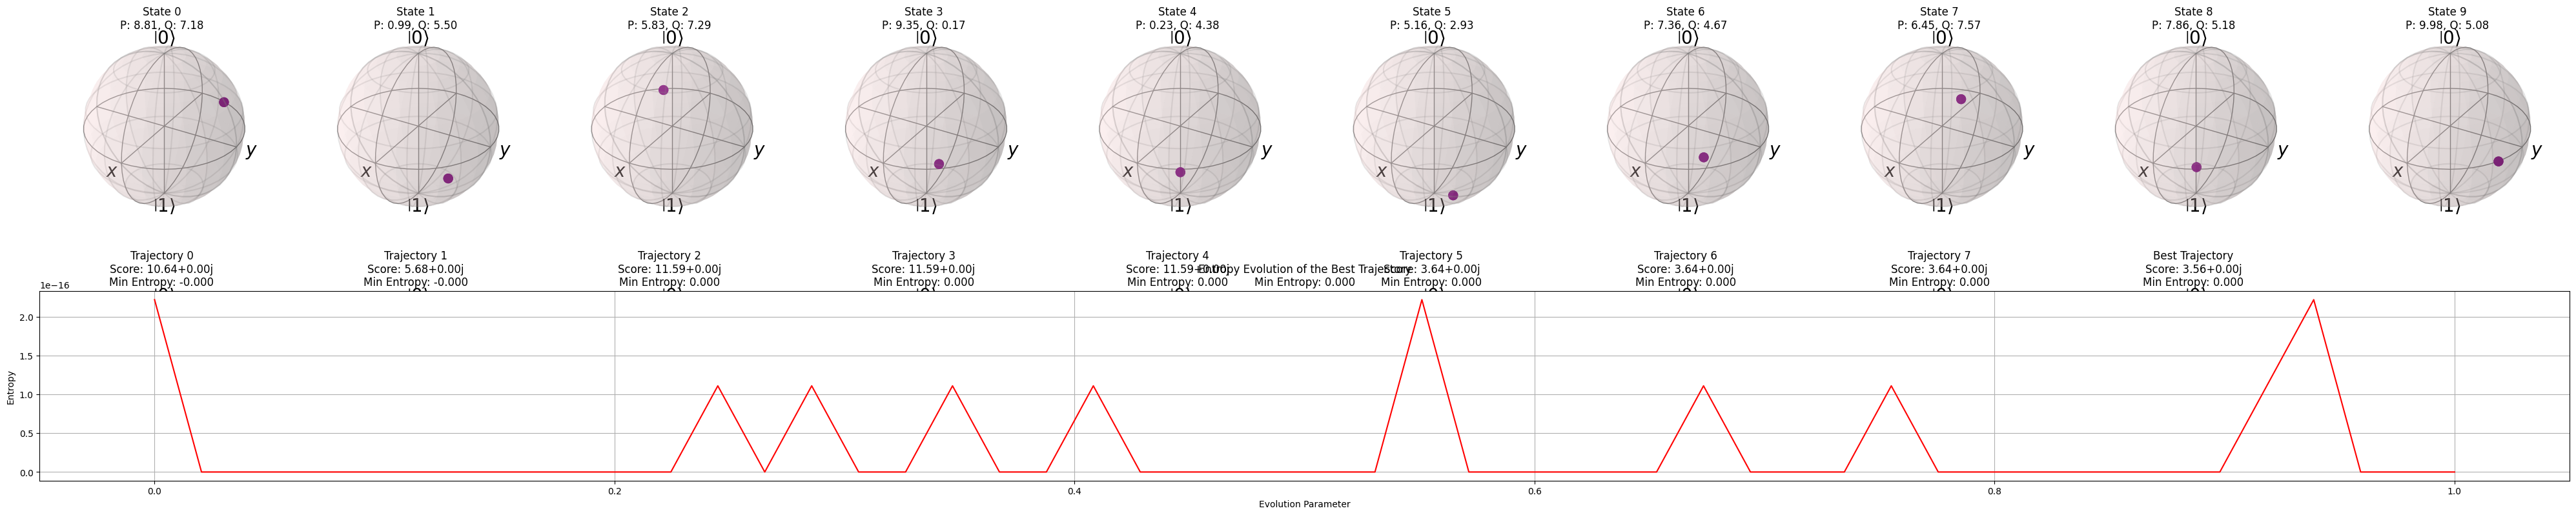
\includegraphics[width=0.9\linewidth]{images/nrqm(1).png} 
    \caption{Trajectory weighted on entropy of mixture states}
    \label{fig:trajwegh}
\end{figure}
The image shows a simulation of non relativistic quantum management. The first line reports the outcome of Bloch vectors in Bloch spheres associated to a particular phase of the project, in an absolute time. The second line reports the value of entropy, thus measuring the best trajectory: where it minimizes, the best trajectory is chosen.
\newpage
\subsubsection{Relativistic Quantum Management}
\label{rqmsob}
Going further in the analysis of quantum management, I will show a variation of quantum management adopting a combination of quantum mechanics and the special relativity theoretical framework. Special relativity is a physical theory formulated by Albert Einstein in 1905. It describes the relationship between space and time and how they are affected by motion, particularly at very high speeds. The theory is built on two fundamental postulates:

\begin{enumerate}
    \item \textbf{The principle of relativity:} The laws of physics are the same for all observers in uniform motion (i.e., not accelerating).
    \item \textbf{The constancy of the speed of light:} The speed of light in a vacuum ($c$) is the same for all observers, regardless of their motion or the motion of the light source.
\end{enumerate}

These two simple ideas lead to some profound and counter-intuitive consequences for our understanding of space and time.

\begin{itemize}
    \item \textbf{Time Dilation:} Moving clocks run slower than stationary clocks. This means that if you were to travel at a very high speed, time would pass more slowly for you than for someone who remained stationary.
    \item \textbf{Length Contraction:} The length of a moving object appears to shrink in the direction of its motion. The faster an object moves, the shorter it appears to an observer.
    \item \textbf{Relativistic Mass:} As an object's speed increases, its mass also increases. This is why it would take an infinite amount of energy to accelerate a massive object to the speed of light, making it an impossible feat.
    \item \textbf{Mass-Energy Equivalence ($E=mc^2$):} This is the most famous outcome of special relativity. It states that mass and energy are two different forms of the same thing. A small amount of mass can be converted into an enormous amount of energy, and vice versa. This principle is the foundation for nuclear power and the atomic bomb.
\end{itemize}
Combining quantum mechanics and special relativity leads to Quantum Field Theory (QFT), the most successful theory for describing the universe's smallest particles. It was a major step in physics because it addressed a fundamental conflict: quantum mechanics works well for a fixed number of particles, but special relativity tells us that particles can be created and destroyed, as energy can turn into mass.

The Klein-Gordon equation was one of the first relativistic wave equations proposed to describe quantum particles. It was developed to fix some issues with the Schrödinger equation when applied to relativistic particles. While it successfully incorporated special relativity and predicted the existence of antiparticles, it had its own problems, such as yielding negative probability densities, which made it a less-than-perfect solution for single-particle systems. However, it was later understood to correctly describe spin-0 particles (like the Higgs boson) and the Dirac equation, which was developed to describe the electron, a spin-1/2 particle and introducing the concept of antimatter.\\\\
Given that we have the basement to explain the principle ingredients of the Relativistic Quantum Management which are: 
\begin{enumerate}
  \item \textbf{Feynman Path Integral}
  \item \textbf{Density Matrix}
  \item \textbf{Pilot Wave}
  \item \textbf{Entropy}
\end{enumerate}
In the following sections, I will discribe them more in detail.
\newpage
\subsubsection*{First Ingredient: Feynman Path Integral}
The next crucial step in Quantum Field Theory (QFT) was the introduction of a theoretical tool designed to describe the movement and interaction of particles. This tool, known as \textbf{the propagator}, calculates the probability of a particle traveling between an initial and a final point in spacetime, essentially modeling the exchange of information or a force. This is "the propagator" that is a mathematical tool that calculates the probability amplitude for a particle to travel from one point in spacetime to another. 

It's not limited to a single path but accounts for all possible trajectories, including those that seem impossible from a classical perspective. The propagator effectively "integrates" over all these possibilities, weighing each one based on its probability. This is crucial for describing interactions, as it treats the transfer of a force or influence (like the electromagnetic force) as the propagation of a mediating particle (like a photon) between interacting points.

In the context of information and management, the propagator analogy offers a potential way to understand how information travels through a dynamic system, especially under uncertainty. In traditional management, information flows along a fixed hierarchy or predefined communication channels: this is like a particle moving along a single, predetermined path. A propagator-based model of information, however, acknowledges that information doesn't just follow official channels. It can travel through informal networks, be delayed or accelerated by unexpected events, and even take "impossible" paths as new connections are formed. The system must account for all these possibilities, not just the one we expect. Moreover, just as a virtual particle mediates a force in physics, information acts as the mediating "force" that connects different parts of a project or organization. A decision made by one team isn't a simple action; it's a piece of information that "propagates" through the system, influencing other teams, tasks, and stakeholders. The "strength" of this influence depends on the information's content and the nature of the connections, much like a propagator's amplitude depends on the particle's properties and the distance traveled. The points where information is created, interpreted, or acted upon can be seen as the "vertices" in an organizational Feynman diagram.

\begin{figure}[!h]
    \centering
    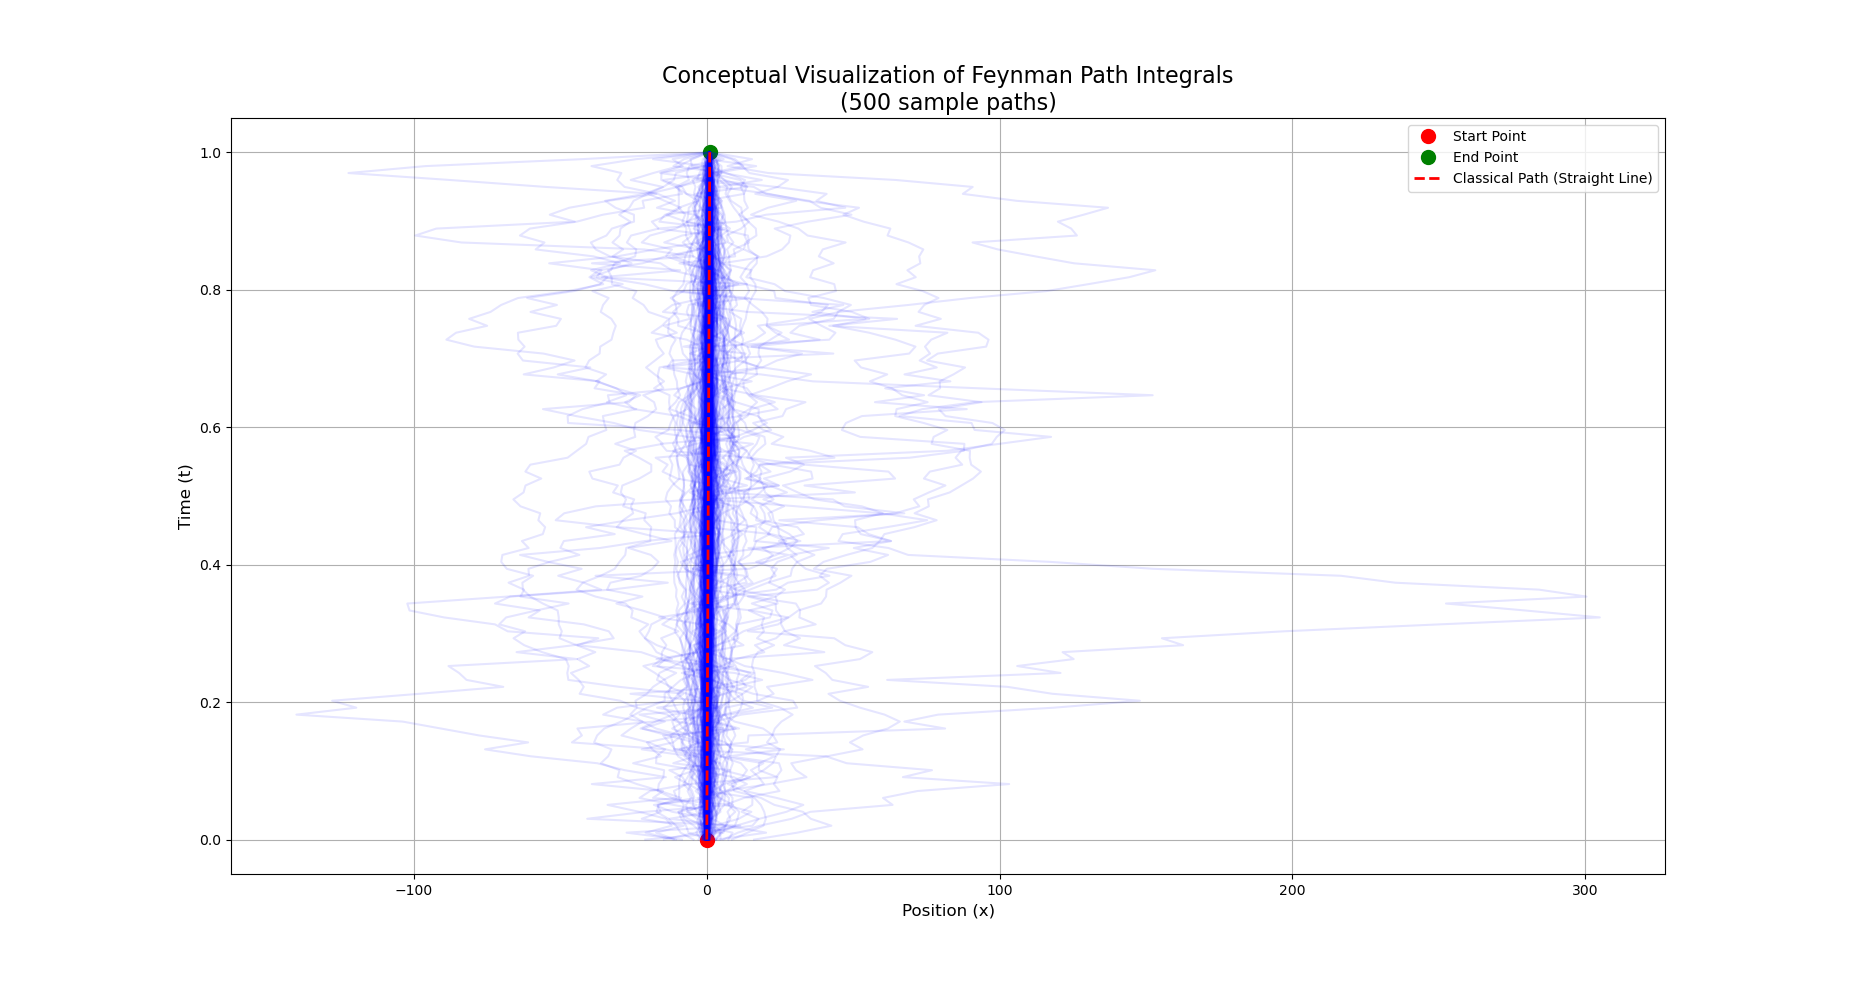
\includegraphics[width=1.0\linewidth]{images/Figure_1.png} 
    \caption{Visualization of Path Integral}
\end{figure}

At these points, information is exchanged, and the state of the system changes. For instance, a meeting where a critical decision is made is a vertex where information from various sources converges and then propagates outward as a new set of instructions or expectations. By viewing information as a propagator, we can move beyond a simple input-output model and better understand how to manage the inherent chaos and uncertainty in complex, interconnected systems.

\begin{figure}[!h]
    \centering
    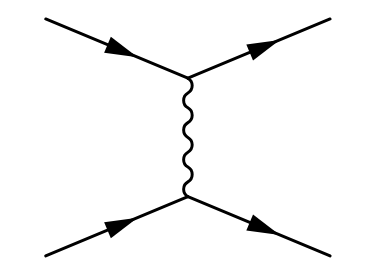
\includegraphics[width=0.6\linewidth]{images/Screenshot 2025-09-09 at 12-32-04 feynmf_package_example_1.pdf.png} 
    \caption{A Feynamn Diagram}
\end{figure}
\newpage
\subsubsection*{Second Ingredient: Densitiy Matrix}
In the context of quantum management, the inherent uncertainty and multiplicity of events can be formalized by viewing information processing through the lens of a propagator, which accounts for all possible intermediate states. However, while intermediate events may be uncertain, a project still requires a coherent path from its inception to its completion. This apparent contradiction—between probabilistic microscopic states and a deterministic macroscopic trajectory—can be resolved by drawing an analogy to the pilot-wave theory of quantum mechanics and density mixture states.
\\An intermediate project state is formally defined by a von Neumann density matrix, denoted by $\rho$. A density matrix describes the statistical state of a quantum system: unlike a pure state, which is represented by a single ket vector ($|\psi\rangle$) and has a definite outcome upon measurement, a mixed state is a statistical ensemble of pure states. The density matrix for a mixed state is a convex combination of the projectors onto the pure states in the ensemble:
$$
\rho = \sum_i p_i |\psi_i\rangle\langle\psi_i|
$$
Here, $p_i$ is the probability of the system being in the pure state $|\psi_i\rangle$, and $\sum_i p_i = 1$. The eigenvalues of $\rho$ represent these probabilities. For a project's sprint, this means that the density matrix $\rho$ represents the project's status as a blend of various possible outcomes, each with a specific probability. For instance, a task can be in a mixed state of "completed" with a certain probability and "incomplete" with another.

The evolution of a project's state over time is governed by the Liouville-von Neumann equation. This equation describes how the density matrix $\rho$ evolves in time:
$$
i\hbar\frac{d\rho}{dt} = [H, \rho]
$$
where $\hbar$ is the reduced Planck constant, $H$ is the Hamiltonian operator representing the "project's energy" or the dynamics of the sprint (e.g., resources, dependencies, and potential risks), and $[H, \rho] = H\rho - \rho H$ is the commutator. This equation encapsulates how the project's state changes based on the interplay between its current state and the forces (the Hamiltonian) acting upon it. The non-commutative nature of the equation highlights how different project factors (represented by components of $H$) can influence the state in a way that depends on the order of their application, which is crucial for complex projects where timing is critical.

For a simple two-state system, such as a task being either "completed" or "incomplete," the project's state can be visualized using the Bloch sphere. A pure state lies on the surface of the sphere, while a mixed state is represented by a point inside the sphere. The center of the sphere represents the maximally mixed state, where there is equal probability for all possible outcomes. The coordinates of a point within the sphere, $(x, y, z)$, are directly related to the density matrix:
$$
\rho = \frac{1}{2}(I + x\sigma_x + y\sigma_y + z\sigma_z)
$$
Here, $I$ is the identity matrix, and $\sigma_x$, $\sigma_y$, $\sigma_z$ are the Pauli matrices. This representation provides a powerful geometrical tool to visualize the evolution of the project's state as a trajectory within the sphere, with the length of the vector from the origin representing the degree of certainty about the project's outcome. As the project progresses and uncertainties are embraced, the state's representation moves from the interior of the sphere towards its surface.

In summary, a sprint's project's status in this model is like a cloud of possibilities, not a single, clear point.
\begin{itemize}
  \item \textbf{Von Neumann Density Matrix (The "Cloud")}: This is a mathematical tool that describes a project's state when its outcome is uncertain. Instead of saying a task is "done" or "not done," it's described as a mix—for example, a 60\% chance of being "done" and a 40\% chance of being "not done." This "cloud" of possibilities is what a density matrix represents;
  
  \item \textbf{Liouville-von Neumann Time Evolution (The "Cloud's Movement")}: This is an equation that explains how the project's state (our "cloud of possibilities") changes over time. It shows how the project's current status and the external factors acting on it (like new problems or risks) cause the cloud to shift and evolve;
  
  \item \textbf{Bloch Sphere (The "Cloud's GPS")}: This is a visual map for simple two-outcome situations (like "task is done" vs. "task is not done"). If the outcome is certain, the project is a point on the surface of the sphere. If the outcome is uncertain, it's a point inside the sphere. As you gain more certainty, the point moves from the inside to the surface of the sphere. It's a way to visually track how close you are to a clear outcome.
\end{itemize}

\begin{figure}[!h]
    \centering
    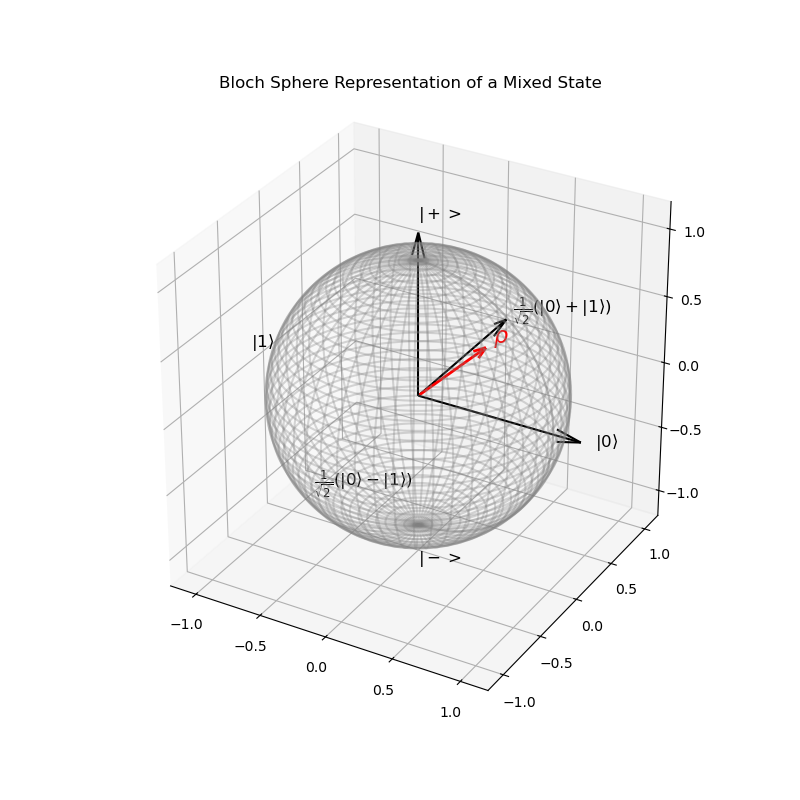
\includegraphics[width=0.9\linewidth]{images/bloch_sphere_mixed_state.png} 
    \caption{Densitiy Mixture State in a Bloch Spheres}
\end{figure}
\newpage
\subsubsection*{Third Ingredient: Pilot Wave}
The Bohm-De Broglie mechanics, offers a deterministic interpretation of quantum mechanics. It posits that particles have definite trajectories, and there's no true randomness or "collapse of the wave function." Instead, the motion of particles is completely determined by their initial positions and a non-local "pilot wave" that guides them. In this framework, the probabilistic nature of quantum states, described by the wave function's squared modulus ($|\psi|^2$), is not fundamental but rather a manifestation of our ignorance of the precise initial conditions.

To formalize this analogy, we can conceptualize the project backlog as the pilot wave. Just as the pilot wave in Bohm-De Broglie mechanics guides the particle's trajectory, the project backlog provides a deterministic line or roadmap for the project, guiding the team's actions from a high-level perspective.

\newpage
\subsubsection*{Fourth Ingredient: Entropy}
In the end, how do I discriminate among trajectories?\\
My theoretical framework is built upon the role of Entropy, Gibbs Energy and the Entalpy in Statistical Mechanics.
\textbf{The Gibbs free energy} is the key to understanding a project's spontaneity. It tells us whether a project will progress naturally or if it will be an uphill battle. The governing equation is:

$$ \Delta G = \Delta H - T\Delta S $$

\begin{itemize}
    \item A \textbf{negative $\Delta G$} indicates a \textbf{spontaneous} trajectory. This is the ideal path, as the project naturally moves toward a stable, successful outcome without needing excessive external effort.
    \item A \textbf{positive $\Delta G$} indicates a \textbf{non-spontaneous} trajectory. This path requires continuous effort and resources to be pushed forward, signaling potential failure or high costs.
    \item A $\Delta G$ of zero means the project is in a state of \textbf{equilibrium}, with no tendency to change on its own.
\end{itemize}


\textbf{Enthalpy} represents the total energy or effort within the project. It includes resources, manpower, and risks.

\begin{itemize}
    \item A \textbf{negative $\Delta H$} (exothermic) signifies a trajectory that \textbf{releases energy}. This might be a task that becomes easier to complete than expected, requiring less effort. This makes the project more likely to be spontaneous.
    \item A \textbf{positive $\Delta H$} (endothermic) means the trajectory \textbf{absorbs energy}. This happens when a task requires more resources or effort than planned, making the project less likely to be spontaneous.
\end{itemize}

\textbf{Entropy} measures the \textbf{disorder or uncertainty} within a project. It quantifies the number of possible outcomes at any given moment.

\begin{itemize}
    \item \textbf{Low Entropy ($S$)}: A state of high order and certainty. A project with low entropy has a well-defined outcome with few remaining possibilities. This is a desirable final state, as it means the outcome is predictable and stable. For example, a task that is 99\% complete with one final, known step has low entropy.
    \item \textbf{High Entropy ($S$)}: A state of high disorder and uncertainty. This corresponds to a project with many possible outcomes. A task with many unresolved dependencies or risks is in a high-entropy state. While often seen as negative, a project that increases in entropy ($\Delta S > 0$) can be more spontaneous, as it moves toward a more "disordered" state of possibilities, which might include new, resilient paths to success.
\end{itemize}

In the Gibbs equation, the entropy term ($T\Delta S$) competes directly with the enthalpy term ($\Delta H$). To achieve a spontaneous trajectory ($\Delta G < 0$), a project must either release enough energy ($\Delta H$ is very negative) or its uncertainties must be managed in a way that contributes to a more stable final state.

\subsubsection*{Mathematical Domain of Relativistic Quantum Management}
I thought as the mathematical domain for this model a Sobolev space. These spaces are a generalization of Euclidean spaces that are essential for solving differential equations, particularly in situations where solutions may not be perfectly smooth or differentiable in a classical sense. By using weak derivatives, Sobolev spaces provide the ideal framework to model the pilot wave, allowing for a continuous, deterministic trajectory (the project backlog) to coexist with the seemingly probabilistic and non-deterministic outcomes of individual tasks (the sprint backlos). The evolution of the project's macroscopic trajectory (the pilot wave/backlog) can be described by a differential equation whose solutions are found via a weak formulation. 

This approach is crucial because it allows us to analyze the project's overall path even if the individual steps—the "intermediate states"—are discrete or exhibit sharp, non-differentiable changes. The Gateaux/Fréchet differentiation further allows us to analyze the sensitivity of the overall trajectory to these local, uncertain events. Within this framework, the probabilistic nature of local project outcomes (the "quantum states") is not a fundamental property of the system. Instead, it is the observable manifestation of where the project currently sits on its deterministic, high-level trajectory. The project's progression is thus the result of a deterministic path through a space governed by the pilot wave (the backlog), even though the precise details of that path may be hidden from us.

The use of Sobolev spaces provides the necessary mathematical rigor to formalize the pilot-wave analogy. It allows for the co-existence of a continuous, deterministic macroscopic trajectory (the pilot wave/backlog) with the probabilistic, microscopic quantum states of individual tasks, effectively bridging the conceptual gap between the classical, top-down view of project management and the quantum, non-deterministic reality of complex processes. In particular, the pilot-wave theory of quantum mechanics (Bohmian mechanics) \cite{bohm1952suggested1} provides a deterministic interpretation of quantum mechanics such that the motion of the particles is completely determined by their initial positions and the pilot wave. This means there is no fundamental randomness or "collapse of the wave function." In this theory, indeed, a particle has a definite, deterministic trajectory, guided by a non-local "pilot wave" that satisfies a generalized form of the Schrödinger equation.

Within a Sobolev space \cite{sobolev1938}, the pilot wave itself can be conceptualized as a continuous curve or a trajectory. Its evolution can be described by a differential equation whose solutions are found via a weak formulation. The probabilistic nature of quantum states, represented by the squared modulus of the wave function $|\psi|^2$, is also contained within this framework. The stochastic outcomes of local measurements are not truly random but are the observable manifestations of the system's position on a deterministic trajectory within a space governed by this non-local "pilot wave" \cite{bohm1952suggested1}, \cite{debroglie1927nouvelle}.

In summary, I reconsider the Sobolev space, equipped with weak derivatives and Gateaux/Fréchet differentiation \cite{frechet1909calcul}, \cite{gateaux1919fonctions}, provides the proper mathematical domain for formalizing the pilot-wave theory. It allows for the co-existence of a continuous, deterministic macroscopic trajectory (the pilot wave) with the probabilistic, intermediate microscopic quantum states, thereby bridging the conceptual gap between classical and quantum descriptions of motion.
\newpage
\subsubsection*{Relativistic Quantum Management within a Deterministic and Non-Deterministic approach}
\label{RQM}
A fundamental assumption in classical management is that time is an absolute and constant resource. This perspective, however, is at odds with physics and psychology, for example, the perception and flow of time are highly relative. The linear, uniform march of an "absolute" time ($t_{absolute}$) is replaced by the complex, subjective experience of "relative" time ($t_{relative}$) within \textit{interacting systems}.
 
 Mathematically, this can be represented as a shift from a single, isolated system to a complex web of interacting systems:
 $$ \text{single living ecosystem}(t_{absolute}) \rightarrow \text{interacting and living ecosystems}(t_{relative}) $$

\begin{itemize}
\item $\text{single living ecosystem}(t_{absolute})$: This represents the classical, Newtonian management view. The project or organization is a single, isolated system operating within a universal, unchangeable timeline. All tasks, phases, and deadlines are planned and measured against this absolute clock. The assumption is that a task will always take a fixed amount of time, regardless of external factors.

\item $\text{interacting and living ecosystems}(t_{\text{relative}})$: This represents the modern, agile, or ``quantum'' management view. The organization is a complex web of interconnected and interdependent subsystems (teams, departments, projects). Each of these ecosystems has its own internal ``relative time.'' For example, a team in a state of ``flow'' might perceive time as passing quickly, while a team struggling with a bottleneck might feel time is dragging. The overall project timeline is no longer a fixed line but is instead a product of the relative, subjective, and interactive experiences within these various subsystems.

\end{itemize}
 
 This presents a critical challenge for management theory: how can I structure and plan a process when our most crucial resource, time, is not a constant but a variable subject to observer-dependent perception?
 

 
 To address the relativity of time in management, I can draw a powerful analogy from the development of relativistic quantum mechanics in physics.
 

 
 The journey from a non-relativistic to a relativistic framework in physics is a useful model for management.
 
 \begin{itemize}
 	\item \textbf{Non-relativistic Schrödinger Equation}: The non-relativistic Schrödinger equation contains a first-order time derivative and a second-order spatial derivative. This asymmetry means that time and space are not treated equally, which violates the principles of special relativity, where space and time must be treated symmetrically.
 	\item \textbf{Klein–Gordon Equation}: The first attempt at a relativistic quantum equation was the Klein–Gordon equation, which has second-order derivatives for both space and time. However, it faced a major physical problem: it allowed for negative probability densities, which are not physically viable. In modern physics, this equation is now understood to describe spin-0 (scalar) particles.
 	\item \textbf{Dirac Equation}: The problem was resolved by Paul Dirac, who developed the Dirac equation. This formulation is first-order in both time and space derivatives, successfully unifying special relativity and quantum mechanics and describing the behavior of spin-1/2 particles (like electrons).
 \end{itemize}
 
 This progression serves as an analogy for management. The shift from a non-relativistic Schrödinger-like model (with absolute time) to a relativistic Dirac-like model mirrors the transition from a classical management paradigm to a modern framework where time, like space, is a dynamic and relative variable. A relativistic approach is essential for a comprehensive and accurate understanding of a management process where the perception of time is inherently relative.
 
 
 
 Special relativity relies on \textbf{Lorentz transformations} to describe how measurements of space and time change between different inertial reference frames (frames that are not accelerating). The transformations are as follows:
 \begin{align*}
 ct' &= c \cosh(\theta) t + \sinh(\theta) x \\
 x' &= c \sinh(\theta) t + \cosh(\theta) x \\
 y' &= y \\
 z' &= z
 \end{align*}
 
 I can also write the transformation for time explicitly as:
 $$ t' = \cosh(\theta) t + \sinh(\theta) \frac{x}{c} $$
 
 Here, the variables are defined as:
 \begin{itemize}
 	\item $t'$ and $x'$: The time and position coordinates in a new, moving reference frame.
 	\item $t$ and $x$: The time and position coordinates in the original, stationary reference frame.
 	\item $c$: The speed of light in a vacuum, a fundamental physical constant.
 	\item $\theta$: The rapidity, a parameter that represents the relative velocity between the two reference frames. It is related to the relative velocity $v$ by the equation $\tanh(\theta) = v/c$.
 	\item $\cosh$ and $\sinh$: The hyperbolic cosine and hyperbolic sine functions, respectively. They are used in Lorentz transformations instead of the trigonometric functions (like cosine and sine) used for spatial rotations.
 \end{itemize}
 
 In a more general context, an observer (Observer X) defines the time interval between two events, A and B, as the quantity $\Delta t = t_B - t_A$, which is measured using their own set of axes and their own frame of reference. This is the essence of time being relative and dependent on the observer.


Imagine a project as a journey from a starting point to a destination. In traditional management, I might think of this as a single, predetermined path. In this new framework, I propose that a project is more like a global pilot wave, a concept from quantum mechanics that guides the possible "paths" or scenarios the project can take. This wave, which I call the project backlog, contains all potential tasks and their relationships.

\begin{equation}
\psi_{\text{projectBacklog}} = e^{iS_{\text{sprint}}/\text{task}}
\end{equation}
Here, $\psi_{projectBacklog}$ represents the overall state of the project backlog. This is a complex number that captures the potential of the project. $S_{sprint}$ is the phase of this wave, a measure of the project's progress and state. The 'task' variable scales this phase, making the equation's units consistent. This equation suggests that the state of the project is not just a list of items but a dynamic entity with a "phase" that evolves.

\subsubsection*{The Velocity of the Project}
Just as a particle has a velocity, I can define the velocity of the project backlog ($v_{projectBacklog}$). This velocity isn't about physical speed but about the rate at which the project moves through its possible states.

\begin{equation}
v_{\text{projectBacklog}} = \frac{dq}{dt} = \frac{\text{Task}}{\text{Quality}} \nabla S_{\text{sprint}}(P, Q)
\end{equation}
In this equation, q(t) is the project's trajectory in its "scenario space." $\nabla_{S_{sprint}}(P,Q)$is the gradient of the project's phase, which depends on two key factors: Priority (P) and Quality (Q). The gradient shows the direction and rate of the steepest change in the project's state. The term QualityTask acts as a scaling factor, indicating that the speed of progress is influenced by the size of the task and the required quality. A project with high priority and high quality requirements will have a different "velocity" than one with low priority and lower quality standards.

\subsubsection*{The Spread of the Project Wave}
In physics, diffusion describes how a substance spreads out. In my model, diffusion of the project wave (J) describes how information, changes, and tasks spread throughout the project. It is like a measure of how new work or new ideas propagate through the team and the backlog.

\begin{equation}
J = w(P, Q)_i \frac{d \rho_{\text{sprint}_i}}{dt}
\end{equation}
This equation is inspired by Fick's law of diffusion. J is the diffusion, which is influenced by two things:
\begin{itemize}
\item $w(P,Q)_i$: a weight of priority and quality for a specific task (i). A high-priority, high-quality task will have a different weight than a low-priority one.
\item $\frac{d \rho{\text{sprint}_i}}{dt}$: the rate of change of the mixture density state of a sprint backlog. This represents how the composition of a sprint (e.g., the mix of high- and low-priority tasks) changes over time.
\end{itemize}
This suggests that how fast a project diffuses and adapts is determined by the specific blend of tasks in its sprints and their associated priorities and quality standards.

\subsubsection*{Entropy and Project Disorder}
Entropy in physics is a measure of disorder or randomness. In this framework, project entropy ($S_{project}$) measures the disorder or uncertainty in a project. A project with many competing priorities and a lack of clear direction would have high entropy. The goal is to reduce this to a more ordered, manageable state (S=0).

\begin{equation}
dS_{\text{project}} = \sum_i (d\rho_i \cdot p_i \cdot w(P, Q)i) t{\text{relative}}
\end{equation}
This equation shows the change in project entropy. It is a sum over all tasks (i), where:
\begin{itemize}
\item $d\rho_i$: the change in the mixture state for a specific task.
\item $\rho_i$: the probability of that specific task state.
\item $w(P,Q)_i$: the priority and quality weight for the task.
\item $t_{relative}$: a relative time factor, which scales the entropy based on the project timeline.
\end{itemize}
The change in the mixture state is governed by a principle similar to the von Neumann equation, which is inspired by Liouville's theorem.

\begin{equation}
d\rho_i = \frac{\partial{\rho_i}}{\partial t} + {H, \rho_i} =0
\end{equation}
This equation states that the mixture of tasks in a sprint is conserved over time unless acted upon by outside forces. {H,$\rho_i$} is a "Poisson bracket" that represents the internal dynamics and relationships within the project, like how a change in one task affects another. A system where $d\rho_i=0$ is in a stable state.

\subsubsection*{Free Energy: The Available Project Energy}
In thermodynamics, free energy is the energy available to do useful work. I can apply this concept to projects.

\begin{itemize}
\item Helmholtz Free Energy (A): This is the energy available for work when the project's scope and environment are constant.
\begin{equation}
A = U - TS
\end{equation}
Here, U is the internal energy (e.g., the effort and resources invested), and TS is the energy "locked up" in project disorder (S) and its internal "temperature" (T). Projects naturally move toward a state of minimum Helmholtz free energy, meaning they seek to complete work with the least amount of wasted effort or internal friction.
\item Gibbs Free Energy (G): This is a more practical measure for projects that are influenced by external factors, like stakeholder pressure or market changes (analogous to constant pressure in physics).
\begin{equation}
G = H - TS
\end{equation}
This equation includes the enthalpy (H), which accounts for both internal energy and the "work" needed to handle external pressures. A project with external constraints will spontaneously move towards a state of minimum Gibbs free energy, seeking to accomplish its goals efficiently while adapting to the external environment.
\end{itemize}

\subsubsection*{The Path Integral: A Sum Over All Scenarios}
Feynman's path integral is a revolutionary concept in physics that suggests a particle doesn't take one path but all possible paths simultaneously. 

In my model, I use this idea to describe a project's evolution. A project doesn't have a single, predetermined outcome; it exists as a superposition of all possible scenarios, or "paths," it could take.

\begin{equation}
\Phi_{\text{carry}}(q_b, t_b; q_a, t_a) = \int_{q(t_a)=q_a; q(t_b)=q_b} \mathcal{D}^f \text{scenario}(\cdot) e^{\frac{i}{\text{adaptiveness}} S_{\text{sprint}}}
\end{equation}
\begin{itemize}
\item $\phi$: This symbol, inspired by the Greek word $\phi \epsilon \rho \omega$ (phero), meaning "to carry," represents the total outcome of the project.
\item The Integral ($\int$): In simple terms, this signifies a "sum of all possibilities." Instead of trying to find the one "right" path, a Quantum Manager considers every potential project scenario.
\item $\int Dfscenario()$: This is the path integral, representing a sum over an infinite number of possible project scenarios, from a starting state ($q_a$) at time ($t_a$) to an ending state ($q_b$) at time ($t_b$).
\item $e^{\frac{i}{adaptiveness}S_{sprint}}$: This term assigns a complex "weight" to each scenario based on the project's action ($S_{sprint}$) and a crucial factor: adaptiveness.
\end{itemize}
The factor $\hbar$ in quantum mechanics, often called the quantum factor, is the fundamental scale of quantum effects. Here, it is replaced by adaptiveness. This is the key ingredient that makes a management system "quantum."

\begin{itemize}
\item What is Adaptiveness? In this framework, adaptiveness is the ability of an organization to sense, respond, and learn from its environment. It is the quantum factor that allows the project to explore all possible paths and find the most efficient on
\item Adaptiveness is Crucial: If adaptiveness is zero (a traditional, rigid organization), the path integral follows the classical limit, and the project is forced down a single, predetermined path, like a classical, Newtonian system. A quantum organization, with high adaptiveness, remains flexible and can pivot based on new information, allowing for a more dynamic and successful project.
\end{itemize}

\subsubsection*{Measuring Adaptiveness}
Measuring adaptiveness requires a new set of metrics. Instead of just focusing on final output, we should look at the processes and behaviors that enable a team to change and learn. These metrics might include:
\begin{itemize}
\item Speed of Response to Change: How quickly a team adjusts its priorities after a new insight or stakeholder feedback.
\item Learning Rate: How fast the team integrates new information and applies it to its work.
\item Innovation Rate: The frequency of new ideas and creative solutions emerging from the team.
\end{itemize}

In this quantum management model, time, cost, and quality are not static variables but are dynamically linked to adaptiveness. The project's success is not just about what is delivered, but how well the organization "carried" the project through all its possible scenarios by being a truly complex adaptive system.

 
 Adaptiveness can be measured by how quickly an organization can recognize and respond to a change.
 \begin{itemize}
 	\item \textbf{Lag Time}: The time elapsed between a significant market change (e.g., a competitor's new product, a shift in customer demand) and the organization's strategic response. A shorter lag time indicates higher adaptiveness.
 	\item \textbf{Resource Reallocation Rate}: The speed and efficiency with which resources (people, budget, technology) can be moved from one project or department to another in response to new priorities. This can be measured as the time required to reallocate a certain percentage of the budget or a number of employees.
 \end{itemize}
 

 
 An adaptive organization is one that is constantly learning and iterating. Metrics in this area focus on the organization's ability to generate new ideas and apply them.
 \begin{itemize}
 	\item \textbf{Idea-to-Implementation Cycle}: The average time it takes for a new idea to go from conception to a fully implemented product or service. Shorter cycles are indicative of a more adaptive and flexible process.
 	\item \textbf{Experimentation Rate}: The number of new projects, pilots, or experiments initiated per quarter or year, relative to the total number of projects. A high experimentation rate suggests a culture that embraces trial and error.
 	\item \textbf{Failure-to-Learning Ratio}: A qualitative or quantitative measure of how well the organization learns from its failures. This can be assessed through post-mortem analyses, a culture of psychological safety, and the institutionalization of lessons learned.
 \end{itemize}
 
 
 Resilience is the ability to withstand shocks and recover quickly, while agility is the ability to pivot and change direction.
 \begin{itemize}
 	\item \textbf{Resilience Index}: A composite score based on factors such as supply chain flexibility, financial liquidity, and employee well-being, which collectively indicate the organization's ability to absorb unexpected shocks.
 	\item \textbf{Organizational Agility Score}: This can be measured through surveys that assess employee perceptions of the organization's ability to respond quickly to change, clarity of communication during transitions, and the flexibility of internal processes.
 \end{itemize}
 
  

 
 By viewing adaptiveness as the core quantum variable in management, organizations can move beyond a rigid, classical approach to a more fluid, responsive one. The metrics outlined above provide a framework for quantifying this crucial quality, allowing managers to measure not just what is being produced, but the organization's capacity to evolve and thrive in a relative, uncertain environment.
 

\subsubsection*{The Core Actors in Quantum Project Management}
In this model, the project team is seen as a system of interacting parts, much like a quantum system. The key roles are:
\begin{itemize}
\item \textbf{Product Owner}: This person defines the what and why of the project, representing the customer's needs and vision. They are the source of the project's purpose and direction.
\item \textbf{Scrum Master}: This role is the "quantum regulator," ensuring the team follows the processes and removes obstacles. They manage the internal team dynamics and ensure smooth operation.
\item \textbf{Development Team}: The "quantum workers" who transform the project vision into reality. They are the ones who create and build the product.
\item \textbf{Quantum Manager}: This new, pivotal role is responsible for the overall quality and adaptiveness of the project. Unlike a traditional manager who dictates tasks, the Quantum Manager is a facilitator of the entire "pilot wave," ensuring the project can navigate its multiple possible scenarios effectively. They manage the system, not just the people.
\end{itemize}

\subsubsection*{The Mathematical Blueprint of Management Paradigms}
The evolution of project management can be described using mathematical groups, which are structures that describe symmetry and transformations. This is a powerful way to visualize how a project's flexibility and complexity increase.

\begin{equation}
\mathbb{R/Z} \times SO(2) \times SO(3) \times SO(3, 1) 
\end{equation}

Let's break down each component of this equation:
\begin{itemize}
\item R/Z Newtonian Management: This represents traditional, "waterfall" project management.
\begin{itemize}
\item R/Z is a mathematical group that describes a one-dimensional, linear process that repeats.
\item Analogy: The project moves in a single, predictable line from start to finish, with a fixed sequence of steps. There is no room for change or adaptation. This is a very rigid, low-adaptiveness model.
\end{itemize}
\item SO(2) Agile Management: This represents the transition to Agile methodologies.
\begin{itemize}
\item SO(2) is the group of all rotations in a two-dimensional plane.
\item Analogy: Think of an Agile sprint. The project is not a straight line but a circle. Each sprint is a rotation where the team completes a cycle of planning, execution, and review. This allows for feedback and small adjustments, making it more flexible than the Newtonian model. However, it is still limited in its degrees of freedom.
\end{itemize}
\item SO(3) Non-Relativistic Quantum Management: This is the next level of complexity, where the project begins to behave like a quantum system.
\begin{itemize}
\item SO(3) is the group of all rotations in three-dimensional space.
\item Analogy: The managemet is here characterized by three properties: $time_{absolute}$, cost and quality. This represents the ability to adapt to changes in scope, priority, and team composition. This is a more dynamic, "non-relativistic" model because it doesn't yet account for the ultimate constraints of the project.
\end{itemize}
\item SO(3,1) Relativistic Quantum Management: This represents the most advanced, fully adaptive project management model.
\begin{itemize}
\item SO(3,1) is the Lorentz group, which describes the symmetries of spacetime in Einstein's theory of special relativity. It includes rotations in three spatial dimensions and transformations in time.
\item Analogy: This is the ultimate adaptive system. The project is no longer just a physical entity but a dynamic "spacetime" continuum. All variables quality, cost, and $time_{sprint}$ must deal with the flowing of a relative global time.
\end{itemize}
\end{itemize}

\begin{comment}
\subsubsection*{A Simplified Mathematical View}

A different, more fundamental way to look at this is through a different set of mathematical groups:

\begin{equation}
sp(1) \times S \times SO(3) \times SO(3, 1)
\end{equation}

The following describes the same evolution but with a slightly different focus.
\begin{itemize}
\item sp(1) and SU(2) are groups used to describe quantum spin and particle physics. In my analogy, they represent the intrinsic properties of the project and its tasks, like their "spin" or internal momentum.
\item SO(3) and SO(3,1) remain the same, representing the increasing degrees of freedom and adaptiveness.
\end{itemize}
This emphasizes that a Quantum Manager must consider both the intrinsic nature of the tasks (sp(1) and SU(2)) and the external, dynamic environment (SO(3) and SO(3,1)) to effectively manage the project's "pilot wave" and ensure its success.
\end{comment}

\begin{center}
\begin{figure}[!h]
    \centering
    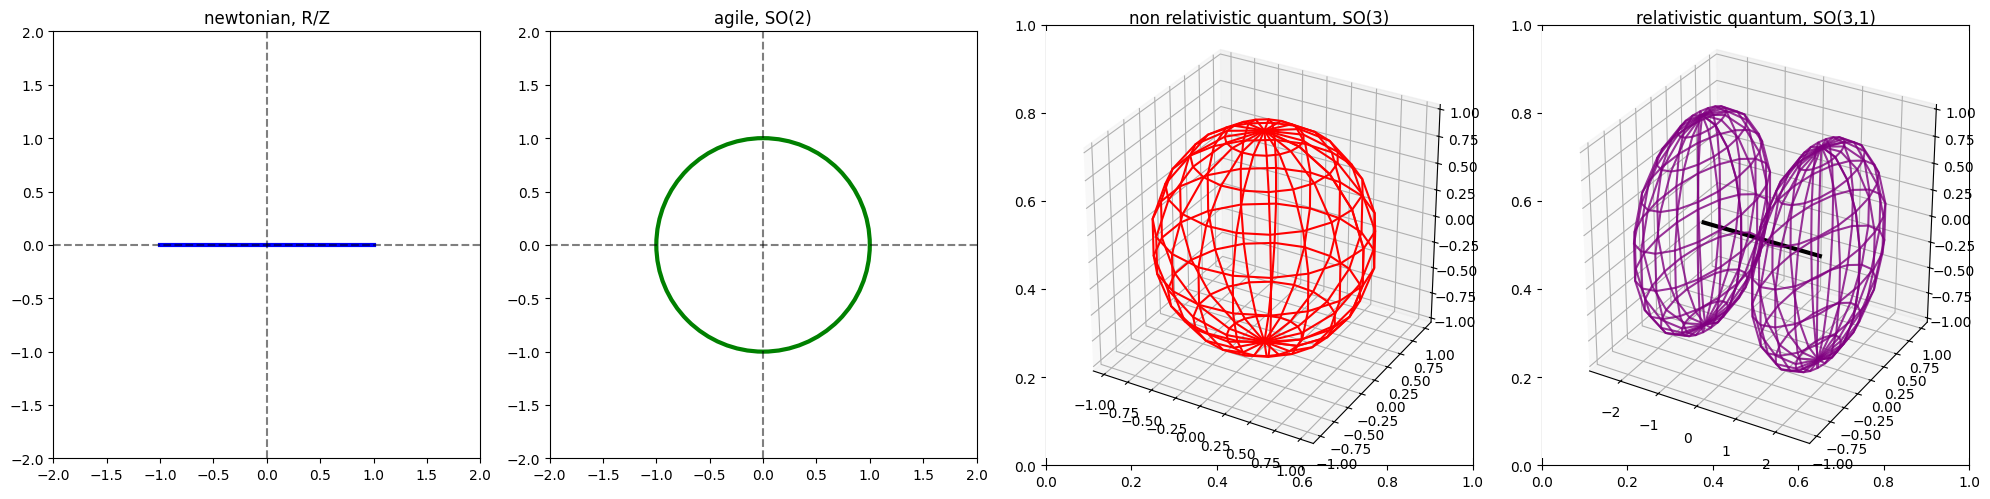
\includegraphics[width=0.9\linewidth]{images/management(1).png}
    \caption{Graphical Representation}
\end{figure}
\end{center}

The following diagram captures the fundamental tension in project management, in the optic of quantum management: the conflict between certainty and uncertainty.

\begin{equation}
\text{Determinism} \xleftrightarrow[\text{Quotient + Emotive + Spiritual Intelligences = Dynamic Intelligence}]{\text{Adaptiveness}} \text{Indeterminism}
\end{equation}

\begin{itemize}
\item \textbf{Determinism}: This represents a project environment that is predictable and certain. In this world, it is possible to define all tasks upfront, and the outcome is largely guaranteed as long as the plan is followed. This is the goal of traditional, "waterfall" project management.
\item \textbf{Indeterminism}: This represents an environment that is unpredictable and uncertain. Changes happen, new information emerges, and the final outcome is not known from the start. This is the reality for most modern, complex projects.
\item \textbf{Adaptiveness}: This is the crucial factor that allows a project to bridge the gap between these two states. It is the ability of a team or organization to sense, respond to, and learn from its environment. Adaptiveness is the mechanism for navigating uncertainty and turning it into a strength.
\item \textbf{Dynamic Intelligence}: This is the collective ability of a team to be adaptive. It is not just about raw intellect. I define it as the sum of three key intelligences:
\begin{itemize}
\item \textbf{Quotient Intelligence (IQ)}: The logical and analytical skills needed to solve problems.
\item \textbf{Emotive Intelligence (EQ)}: The ability to understand and manage emotions, both your own and those of others, which is vital for teamwork.
\item \textbf{Spiritual Intelligence (SQ)}: The ability to find meaning, purpose, and values in work. This provides the motivation to handle ambiguity and stay resilient.
\end{itemize}
\end{itemize}
Essentially, a project can only move from a deterministic, planned state to a successful outcome in an indeterminate world if the team's combined dynamic intelligence fuels its adaptiveness.
\begin{figure}[!ht]
    \centering
    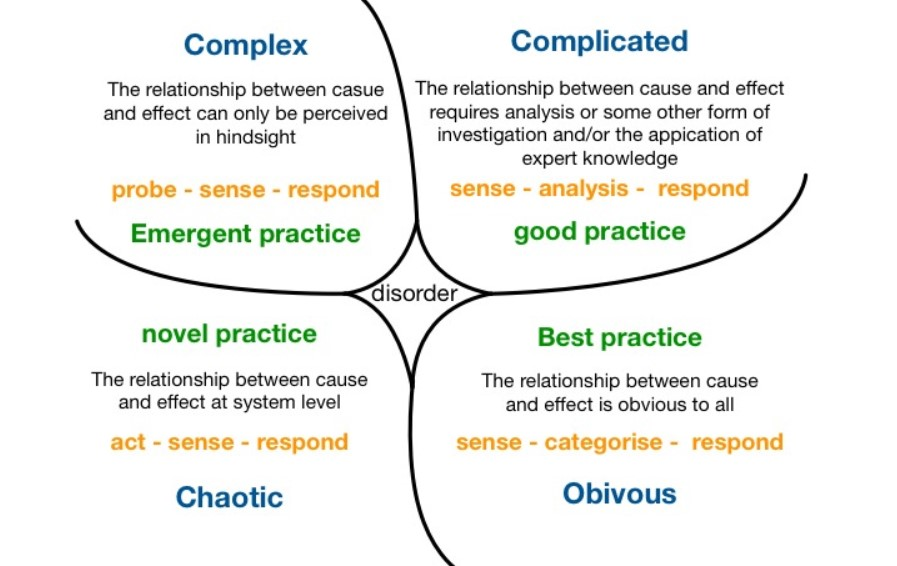
\includegraphics[width=0.5\linewidth]{images/ccco.jpg}
    \caption{From Complicated to Complex: The Cynefin Framework}
\end{figure}

\subsubsection*{From Complicated to Complex: The Cynefin Framework}
The second diagram relates this idea to the Cynefin Framework. The framework, often represented by a diagram with five domains, helps managers understand the type of environment they are in and make appropriate decisions. 

\begin{equation}
\text{complicated-obvious} \xleftrightarrow[\text{}]{\phi \epsilon \rho \omega} \text{complex-chaotic}
\end{equation}

\begin{itemize}
\item \textbf{Complicated-Obvious}: In this state, the project's cause-and-effect relationships are either obvious or can be figured out with expert analysis. We can rely on best practices (obvious) or good practices (complicated) to succeed. This is a predictable, linear world.
\item \textbf{Complex-Chaotic}: Here, the cause-and-effect relationships are only visible in hindsight (complex) or not at all (chaotic). We cannot plan our way through these environments; we must probe, sense, and respond. This is the realm of radical innovation and constant change.
\item $\phi \epsilon \rho \omega$(\textit{phero}): This is the Greek word meaning "to carry" or "to bear," representing the analog Feynman Path Integral from my relativistic quantum management model. It symbolizes the continuous flow of the project, which "carries" the team from a deterministic, predictable state into the unpredictable, complex world.
\end{itemize}
\newpage
\subsubsection*{The Final Evolution: from Non Relativistic to Relativistic Quantum Management}
The final diagram describes the ultimate state of a quantum-managed project, where it becomes a fully adaptive and self-regulating system.

\begin{equation}
\text{Non Relativistic Quantum Management} \xleftrightarrow[\text{}]{\phi \epsilon \rho \omega} \text{Relativistic Quantum Management or Gauge Management}
\end{equation}

\begin{itemize}
\item \textbf{Non-Relativistic Quantum Management}: This is an advanced state where the project team can pivot in three dimensions, making it highly adaptive to changes in quality, priority, and team composition. It is non-relativistic because it does not yet account for the ultimate constraints or "rules" of the system, like a fixed budget or deadline and it relies on an absolute time;
\item \textbf{Relativistic Quantum Management or Gauge Management}: This is the pinnacle of the model. It is a system that is fully aware of its constraints (like a project's budget or deadline, which act like the "speed of light" in physics). The term gauge management comes from gauge theory in physics, which describes how systems can remain consistent and coherent even when they undergo transformations. This is what a quantum-managed project does: it adapts to changes (time, cost, and scope) while maintaining its integrity and purpose. Time is relative.
\end{itemize}
In essence, the pilot wave ($\phi \epsilon \rho \omega$) is the mechanism that takes a project from being merely "highly flexible" (Non-Relativistic) to being a truly self-regulating and coherent system that can handle any change and still achieve its goal (Relativistic). This is the final form of a truly adaptive project organization.

\subsubsection{Code Implementation of Relativistic Quantum Management}
Generated 10 states and 45 trajectories.\\
The best trajectory based on score S (to be minimized) is at index 5.\\
Score S of the best trajectory: 0.0000+0.0000j\\
Minimum entropy of the best trajectory: 0.0000\\
\begin{figure}[!ht]
    \centering
    
\includegraphics[width=0.9\linewidth]{images/rqm(2).png}
    \caption{Relativistic Quantum Mechanics}
\end{figure}
The image of spheres with points on their surfaces provides a powerful visualization of project dynamics. Each sphere represents the total state space of a project at a specific moment in time. The points, or dots, on the surface of each sphere represent the various possible scenarios or states in which the project could be in.

\begin{itemize}
\item \textbf{Initial States (Top Row):} The top row shows a small number of tightly clustered points. Each Bloch sohere, with Bloch vector, represents the phases of a process that is considered.
\item \textbf{Evolving States (Bottom Row):} This shows all the possible positions in which the Bloch vector could be found. As it is not possible ab initio, the best trajectory among all scenarios of positions of Bloch vectors is the one that minimizes the entropy S.
\end{itemize}


Relativistic Quantum Management (RQM) provides the framework for navigating this visual complexity. Instead of trying to control every individual point or scenario, RQM focuses on managing the overall "pilot wave" that governs their evolution. This pilot wave is shaped by the team's adaptiveness, the central factor in this model.

\subsubsection*{Adaptiveness as a Guiding Force}
The spread and movement of the points in the image are not random; they are guided by the project's "pilot wave," which is, in turn, shaped by the team's adaptiveness-the ability to learn, respond, and pivot. The Quantum Manager's primary role is to nurture this adaptiveness. A highly adaptive system can effectively manage the growing number of scenarios, ensuring they collectively converge toward a successful outcome.

\subsubsection*{The Lorentz Group and "Spacetime" in Practice}
RQM, described mathematically by the Lorentz Group (SO(3,1)), incorporates time as an integral dimension, creating a project "spacetime." This means the changing distribution of points in the image is not just a spatial spread but a transformation through time. The project's core goals of time, cost, and scope are interconnected and can be transformed while maintaining the project's overall integrity. For example, if a new high-priority task (a new point) appears, RQM allows the team to coherently adjust the project's timeline or scope, rather than just reacting to an isolated change.

\subsubsection*{From Possibility to Outcome}
The final outcome of the project is not predetermined. The continuous spreading and re-grouping of the points represent the process of a quantum project exploring all possibilities. The final outcome is the single state that is "measured" or collapses from this superposition of possibilities when the project is completed. By managing the pilot wave (project backlog) and encouraging adaptiveness, the Quantum Manager increases the probability that the final measured state is a successful one.

\newpage
\section{$\phi \epsilon \rho \omega$ Quantum Intelligence Neural Network, $\phi QINN$}
\label{sec8}
Relativistic Quantum Management uses the formalization of Path Integral and of Pilot Wave to predict how a local undetermined states could evolve along a global pilot wave that moves from the beginning to the end of a management process. Path Integral requires a relativity formulation. The core concepts of time dilation and length contraction are about how time and space change from a specific observer's perspective in Special Relativity, which provides a great metaphor for how business goals and timelines can seem different depending on your point of view or speed of execution.

The model is a linear stack of layers, with information flowing from the input layer through hidden layers to a single output layer. This feedforward structure is fundamental to its operation. The key components and their mathematical representations are detailed below.\\
The input layer accepts a feature vector $\mathbf{x}$. For each data point (a trajectory), this vector includes flattened Bloch vector components, priority, quality, and a one-hot encoded scenario. The dimensionality of this vector is 160.\\
This is a \textbf{Dense layer} with 128 neurons. It employs a \textbf{ReLU (Rectified Linear Unit)} activation function. The output $h_{1,j}$ for each neuron $j$ is calculated as:
$$h_{1,j} = \text{ReLU}(\mathbf{w}_{1,j} \cdot \mathbf{x} + b_{1,j})$$
where:
\begin{itemize}
    \item $\mathbf{w}_{1,j}$ is the weight vector for the $j$-th neuron.
    \item $\mathbf{x}$ is the input vector.
    \item $b_{1,j}$ is the bias term.
    \item $\text{ReLU}(z) = \max(0, z)$.
\end{itemize}
A \textbf{Dropout layer} with a rate of 0.3 is applied. This technique regularizes the network by randomly setting a fraction of the neuron outputs to zero during training. The output $d_{1,j}$ is given by:
$$d_{1,j} = h_{1,j} \cdot m_j$$
where $m_j$ is a binary mask, with a value of 1 with probability $1 - \text{dropout\_rate}$ (0.7) and 0 with probability $\text{dropout\_rate}$ (0.3). During inference, this layer is inactive.\\
This is another \textbf{Dense layer} with 64 neurons and a \textbf{ReLU} activation function. The output $h_{2,k}$ for each neuron $k$ is based on the output of the previous dropout layer $\mathbf{d}_1$:
$$h_{2,k} = \text{ReLU}(\mathbf{w}_{2,k} \cdot \mathbf{d}_1 + b_{2,k})$$
where $\mathbf{d}_1$ is the vector of outputs from the first dropout layer.\\
Similar to the first, this \textbf{Dropout layer} has a rate of 0.3. The output $d_{2,k}$ is:
$$d_{2,k} = h_{2,k} \cdot m'_k$$
where $m'_k$ is a binary mask.\\
This \textbf{Dense layer} has 32 neurons and a \textbf{ReLU} activation function. The output $h_{3,l}$ for each neuron $l$ is calculated from the outputs of the second dropout layer $\mathbf{d}_2$:
$$h_{3,l} = \text{ReLU}(\mathbf{w}_{3,l} \cdot \mathbf{d}_2 + b_{3,l})$$
\\The final layer is a \textbf{Dense layer} with a single neuron and a \textbf{linear activation function}. This is suitable for regression. The predicted score $\hat{y}$ is:
$$\hat{y} = \mathbf{w}_{4} \cdot \mathbf{h}_3 + b_{4}$$
where $\mathbf{h}_3$ is the vector of outputs from the third hidden layer.
\\The model uses the \textbf{Adam optimizer}, which adaptively adjusts the learning rate. The loss function is \textbf{Mean Squared Error (MSE)}, a standard choice for regression tasks. It measures the average of the squared differences between the actual and predicted values:
$$MSE = \frac{1}{N} \sum_{i=1}^{N} (y_i - \hat{y}_i)^2$$
\\To prevent overfitting, the training process employs an \textbf{EarlyStopping callback}. It monitors the validation loss (\texttt{val\_loss}) and stops training if no improvement is seen for a set number of epochs (patience = 10).\\The \texttt{restore\_best\_weights=True} option ensures the final model uses the weights from the epoch with the lowest validation loss.
\begin{center}
\begin{figure}[!h]
    \centering
    \begin{subfigure}[b]{0.45\linewidth}
        \centering
        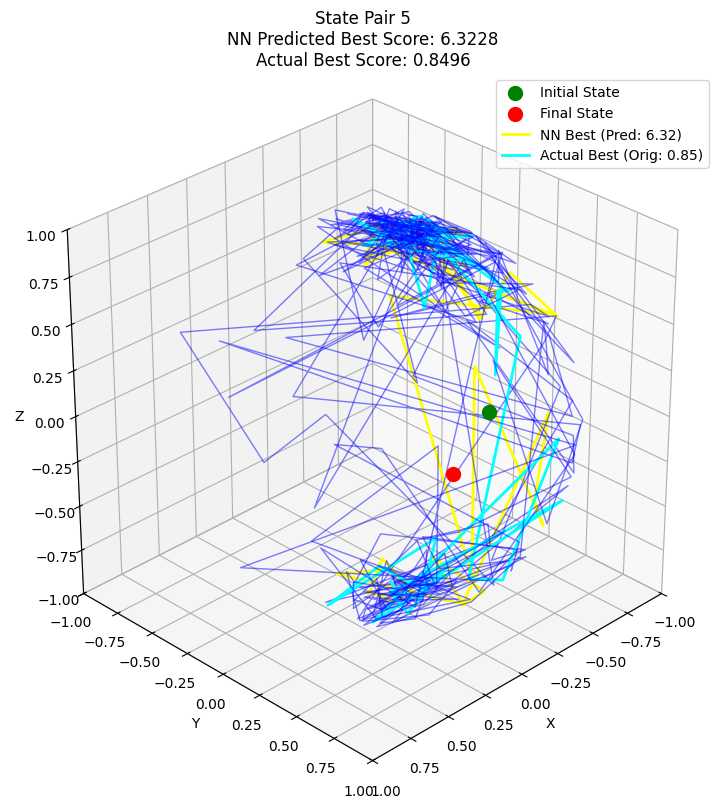
\includegraphics[width=\linewidth]{images/qinn(1).png}
        \caption{Quantum Relativistic Management as a Pilot Wave between initial and final states among many possible quantum mixture density states}
        \label{fig:qinn}
    \end{subfigure}
    \hfill
    \begin{subfigure}[b]{0.45\linewidth}
        \centering
        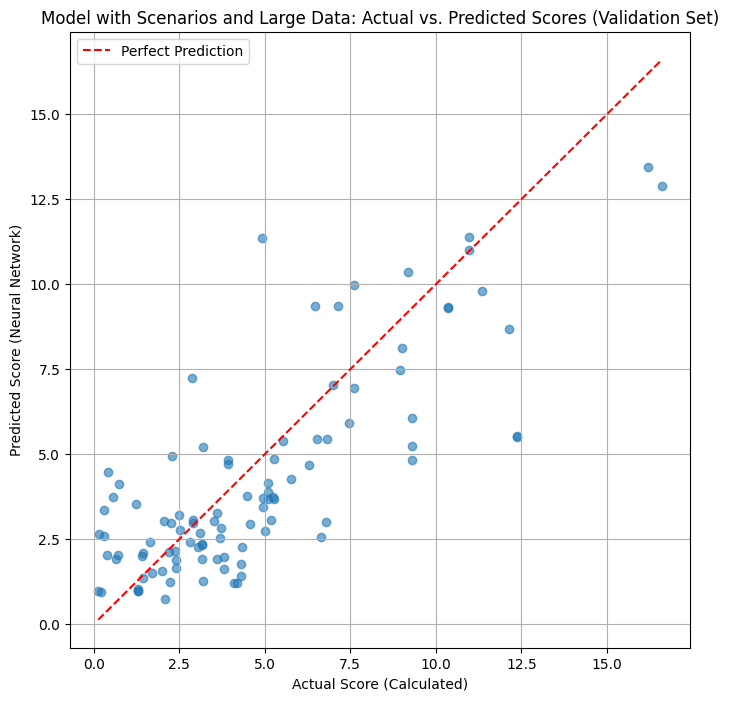
\includegraphics[width=\linewidth]{images/plotPredAct(1).png}
        \caption{Quantum Relativistic Management as a Pilot Wave between initial and final states among many possible quantum mixture density states, plot among predicted and actual trajectory}
        \label{fig:plotPredAct}
    \end{subfigure}
    \caption{Relativistic Quantum Management.}
\end{figure}
\end{center}
The core idea of RQM is that a project doesn't follow a single path. Instead, it exists as a "pilot wave" that contains all possible scenarios from a start point to an end point. Each scenario has a certain probability of happening. The goal of a Quantum Manager is to guide this wave toward the most favorable outcome.

My model, $\phi QINN$, uses a neural network to achieve this. A neural network is a computational system inspired by the human brain. It learns to recognize patterns in data by adjusting the connections between its "neurons." Think of it as a series of filters that process information step-by-step to arrive at a decision or prediction.

The process of using this model for management is as follows:
\begin{itemize}
\item Generate States: I represent different project states (e.g., phases of creating a new insurance product) as mathematical objects called Bloch spheres and Bloch vectors. These spheres and vectors capture the complex relationships and probabilities within each state.
\item Identify All Trajectories: The model considers all possible trajectories—the sequences of states a project could follow from beginning to end.
\item Calculate "Entropy": For each trajectory, the model calculates its entropy, a measure of its disorder or risk. A higher-entropy trajectory is less stable and less likely to succeed.
\item Find the Best Path: The neural network's job is to identify the single, most probable trajectory—the one that minimizes entropy and maximizes the project's chances of success.
\end{itemize}
\newpage
Here the most important steps of the neural network:\\
\begin{equation*}
\begin{gathered}
\text{Bloch Spheres} \\
\downarrow \\
\text{Bloch Vectors (Pauli Matrices)} \\
\downarrow \\
\text{Quantum States} \\
\downarrow \\
\text{Local Trajectories (Global Pilot Wave)} \\
\downarrow \\
\text{Entropy-weighted Trajectories} \\
\downarrow \\
\text{Minimized Entropy (Most Probable Trajectory)}
\end{gathered}
\end{equation*}
\subsubsection*{Building a Neural Network: The Inner Workings}
The neural network used in this framework is a simple, layered structure called a feedforward network. Information flows in one direction: from the input, through a series of "hidden" layers, to the final output.

\subsubsection*{Input Layer: The Data}
The network's journey begins here. The input layer takes in all the information the model needs to make a prediction. This includes:
\begin{itemize}
\item Flattened Bloch vectors: The mathematical representation of each project state.
\item Priority and Quality scores: Key metrics that define the project's goals.
\item Scenario encoding: A way to label the specific trajectory or scenario.
\end{itemize}
This information is combined into a single, comprehensive "feature vector" (a list of numbers) that the network can understand.

\subsubsection*{Hidden Layers: Processing the Information}
The hidden layers are the "brain" of the network, where the "magic" happens.
\begin{itemize}
\item \textbf{Dense Layers:} These layers are the core of the network. Each neuron in a dense layer is connected to every neuron in the previous layer. Think of it as a massive web of connections. Each connection has a weight (its importance) and a bias (an offset). The layer takes the input, multiplies it by the weights, adds the biases, and passes the result to the next layer.
\item \textbf{ReLU Activation:} After the weighted sum, a Rectified Linear Unit (ReLU) function is applied. In simple terms, this function acts as a filter: if the result is positive, it stays the same; if it is negative, it becomes zero. This helps the network learn complex, non-linear patterns.
\item \textbf{Dropout Layers:} To prevent the network from becoming too reliant on specific neurons (a problem called overfitting), a Dropout layer is used. During training, it randomly "shuts off" a fraction of the neurons. This forces the network to learn a more robust, generalized pattern, similar to how a human brain learns to solve a problem from multiple angles.
\end{itemize}
This model has three hidden layers that progressively reduce the number of neurons (from 128 to 64 to 32), distilling the information to its most essential components.

\subsubsection*{Output Layer: The Prediction}
The final dense layer has only one neuron. Its job is to take the distilled information from the hidden layers and produce a single output: a score that represents the predicted "entropy" or risk of the trajectory. A linear activation function is used here because I am predicting a continuous value, not a category.

\subsubsection*{Training the Network}
To make accurate predictions, the network must be trained.
\begin{itemize}
\item Adam Optimizer: This is the network's "teacher." It adaptively adjusts the weights and biases to help the network learn more efficiently.
\item Mean Squared Error (MSE): This is the network's "report card." It measures how close the network's predictions are to the actual, known values. The goal of training is to minimize this score.
\item Early Stopping: This is a key safety measure. It monitors the network's performance during training and stops the process when it no longer shows improvement. This prevents the model from overfitting and ensures I get the best possible result.
\end{itemize}
\newpage
\section{Insurance Leadership and Decision Making within Relativistic Quantum Management Framework}
\label{sec3}
The Relativistic Quantum Management (RQM) framework offers a new paradigm for leaders, especially in complex fields like insurance, by moving beyond traditional, predictable models. This approach embraces the reality of uncertainty and constant change. At its core is the $\phi \epsilon \rho \omega$ (phero) propagator, a concept inspired by physics and used here as a tool for leadership. The name comes from a Greek word meaning "to carry," which perfectly captures the role of a leader who guides a project through a sea of possibilities.

The mathematical formula for this propagator is:
\begin{equation}
\phi\epsilon\rho\omega(q_b, t_b; q_a, t_a) = \int_{q(t_a)=q_a; q(t_b)=q_b} \mathcal{D}^f \text{scenario}(\cdot) e^{\frac{i}{\text{adaptiveness}} S_{\text{sprint}}}
\end{equation}
While this equation may look complex, it provides a powerful mental model for decision-making. Let's break down its components.

\subsubsection*{Deconstructing the Propagator}
\begin{itemize}
\item \textbf{The Propagator ($\phi \epsilon \rho \omega$)}: This represents the overall probability or "strength" of a project successfully moving from a starting point ($q_a$) at time ($t_a$) to an end point ($q_b$) at time ($t_b$). It is a measure of how likely a project is to succeed when considering all the different ways it could unfold.
\item \textbf{The Integral ($\int$)}: In simple terms, this signifies a "sum of all possibilities." Instead of trying to find the one "right" path, a Quantum Manager considers every potential project scenario.
\item \textbf{The "Sum Over Scenarios" ($\int Dfscenario())$}: This part of the formula represents the act of considering every possible scenario or trajectory a project could take. For an insurance company launching a new product, these scenarios could range from a perfect launch to one plagued by regulatory hurdles, market rejection, or unforeseen technical issues.
\item \textbf{The "Weighting" Factor ($e^{\frac{1}{adaptiveness}iS_{sprint}}$)}: This is the most crucial part for leadership. It is a mathematical way of assigning a "score" or "weight" to each scenario. This weight determines how much each scenario contributes to the overall project outcome.
\begin{itemize}
\item \textbf{Project Action ($S_{sprint}$)}: This represents the effort, energy, and resources (the "action") required for a specific scenario to play out.
\item \textbf{Adaptiveness}: This is the most important variable. It is the team's ability to flex, learn, and respond to change. This factor acts as a "quantum" scale. When adaptiveness is high, the project's "pilot wave" can explore a wide range of scenarios, allowing for agile course correction. When adaptiveness is low, the project is forced onto a rigid, single path, making it vulnerable to unexpected challenges. A high adaptiveness value means that even a challenging scenario (with a high $S_{sprint}$) can make a significant and positive contribution to the final outcome.
\end{itemize}
\end{itemize}

\subsubsection*{Decision-Making in Action}
The RQM framework provides leaders with a new set of principles for making decisions:
\begin{itemize}
\item \textbf{Embrace Indeterminism}: The first step for a leader is to accept that a project's future is not set in stone. Instead of creating a single Gantt chart -project management tool that visually represents a project's schedule- and forcing the team to follow it, the leader acknowledges that the project exists as a superposition of all possible scenarios.
\item \textbf{Focus on the Pilot Wave}: A Quantum Manager does not try to micromanage every detail (each "scenario"). Instead, they focus on shaping the overall pilot wave by fostering adaptiveness within the team. This means investing in team skills, establishing clear communication channels, and creating a culture that values learning over rigid adherence to a plan.
\item \textbf{Data-Driven Insight}: Tools like the Quantum-inspired Neural Network ($\phi QINN$) act as a co-pilot. They analyze all possible project trajectories and calculate the "entropy" (risk or disorder) of each. The model then identifies the most probable and least entropic trajectory.
\item \textbf{Informed Decisions}: The leader can use this information to make strategic decisions. For example, if the model shows that a path with high adaptiveness and a high initial cost has the lowest entropy and highest long-run success probability, the leader can confidently choose that path. It is a shift from reactionary to proactive management.
\end{itemize}

The core benefit of this framework is that it helps leaders see a project not just as a series of tasks but as a dynamic system in a "spacetime" continuum where time, cost, and scope are not fixed but are relative to the team's speed and ability to adapt. By nurturing adaptiveness, leaders can increase the probability that their project will "collapse" into a successful outcome.

\subsection{Key Concepts of Relativistic Quantum Management through an Agile Lens}
In the agile methodology, a leader's primary function is to support the team, not to control it. They don't pull the strings; they nurture the environment so the team can grow and thrive on its own. Their key responsibilities include:
\begin{itemize}
\item \textbf{Providing a Clear Vision}: They communicate the overall purpose and goals of the project, ensuring the team understands the "why" behind their work.
\item \textbf{Removing Impediments}: They act as a facilitator, identifying and eliminating any obstacles or blockers that prevent the team from working efficiently.
\item \textbf{Fostering a Culture of Trust and Transparency}: They create a safe environment where team members feel empowered to experiment, learn from mistakes, and communicate openly.
\item \textbf{Coaching and Mentoring}: They help team members develop their skills and grow both individually and as a team.
\item \textbf{Encouraging Collaboration}: They promote cross-functional teamwork and open communication to break down organizational silos.
\end{itemize}

\subsubsection*{Decentralized Decision-Making in Agile}
In an agile environment, decisions aren't made by a single person at the top; they're made by the people who are closest to the work-the team itself. This decentralized approach has several key characteristics:
\begin{itemize}
\item \textbf{Team Autonomy}: Agile teams are self-organizing and have the authority to make decisions about how to best accomplish their tasks. This fosters a strong sense of ownership and accountability.
\item \textbf{Iterative and Incremental}: Decisions are not made all at once in a rigid, long-term plan. Instead, they are made in smaller, more manageable increments. The team works in short cycles, gathers feedback from customers, and then adjusts its course as needed.
\item \textbf{Data-Driven}: Decisions are based on real-time data, customer feedback, and the observed results of the team's work, rather than assumptions or intuition.
\item \textbf{Framework-Specific Tools}: Agile frameworks use specific tools to facilitate decision-making. For example, during Sprint Planning, the team collaboratively decides which backlog items to work on. Tools like the MoSCoW method (Must have, Should have, Could have, Won't have) and Weighted Shortest Job First (WSJF) are used for prioritizing work.
\item \textbf{Transparency and Adaptation}: The process and outcomes of decisions are made transparent to everyone. This allows the team to regularly review its progress and adapt its strategy to become more effective.
\end{itemize}

\subsubsection*{From Agile to Relativistic Quantum Leadership}
The relativistic quantum leader is still a servant leader, but their mindset is more advanced. While the agile leader helps the team navigate a complex landscape, the quantum leader understands that this landscape is not just complex- it is multifaceted and ambiguous, with multiple possibilities existing simultaneously.

Agile tools are the "how," but the relativistic quantum leader possesses the mindset to use those tools to their fullest potential in a truly unpredictable world. They see the project not as a single path but as a wave of possibilities. Their primary role is to ensure the team has the adaptability and skills to navigate this wave toward the most probable successful outcome. This approach recognizes that in today's fast-paced world, the ability to thrive amid ambiguity is the ultimate competitive advantage.

From a relativistic quantum management perspective, the challenge of decision-making is not a linear, rational process. Instead, it is a dynamic and subjective one, influenced by the observer's (leader's) context and biases. 

Indeed, in the process of decision making uncertainty and indetermisn are dominant. Everyone involved should be aware that a decision is rarely a simple, isolated choice based solely on the immediate topic. Instead, it is often driven by a complex web of external factors, which are themselves unpredictable, undeterministic and uncertain. This means that a decision is not a single, definite outcome but rather the result of interacting with a dynamic environment where multiple possibilities exist simultaneously. \textbf{In RQM, the focus shifts from finding the "correct" solution to understanding the full "field of possibilities" and making a choice that accounts for these interconnected, non-deterministic influences}.

For this reason, I thought that a good exisiting theory to reconsider in RQM optic is Kahneman's dual-process and prospect theory \cite{kahneman2011thinking}, a cornerstone of behavioral economics, that provides the psychological foundation for this framework. It delineates two cognitive systems that parallel the relativistic and subjective nature of quantum management, offering a powerful lens for making good leadership decisions.
Daniel Kahneman's work on decision-making, particularly his dual-process theory, provides a powerful lens for understanding the complexities of management. From a management process perspective, his theory explains how leaders and teams make decisions, highlighting the pitfalls of relying solely on intuition while emphasizing the need for structured, deliberate thinking.

In relativistic quantum management, a leader's decision-making process is viewed not as a simple, linear choice but as a complex interaction within a dynamic system. Kahneman's theory of dual cognitive processes provides a powerful framework for this, as it acknowledges the subjective and biased nature of human judgment. By integrating this theory, leaders can move beyond a simplistic, deterministic model of decision-making and embrace a more nuanced, adaptable approach.
\newpage
\subsection{How to Make a Good Leadership Decision through the Prospect Theory Lens}
\label{dual}
The Kahneman's dual-process theory \cite{kahneman2011thinking} delineates two cognitive systems:

\begin{itemize}
    \item \textbf{System 1 (Intuitive Heuristics):} This is the fast, automatic, and often emotionally charged mode of thought. It operates on a basis of pattern recognition and mental shortcuts, or heuristics, allowing for rapid decision-making in familiar contexts. For example, System 1 enables the reflexive act of hitting a car's brakes to avoid a collision.
    \item \textbf{System 2 (Analytical Deliberation):} This is the slow, deliberate, and effortful mode of thought. It is engaged for complex problem-solving, logical reasoning, and conscious self-control. Tasks such as calculating a tax liability or critically evaluating a business proposal are the domain of System 2.
\end{itemize}


The Relativistic Quantum Manager understands that human judgment is not a pristine, rational process but is instead systematically distorted by cognitive biases and random variability, or \textbf{noise} \cite{kahneman2021noise}. Thus, \textbf{RQM embraces uncertainty in the very first step of management: the decision process}.

\begin{itemize}
    \item \textbf{Cognitive Biases ($\sigma_{bias}$):} These are systematic and predictable deviations from rational choice. Kahneman identified several key biases:
    \begin{itemize}
        \item \textbf{Anchoring Bias:} The over-reliance on the initial piece of information presented, which "anchors" subsequent judgments.
        \item \textbf{Availability Heuristic:} The tendency to overestimate the probability of events that are easily recalled or are emotionally vivid.
        \item \textbf{Confirmation Bias:} The selective search for information that confirms one's pre-existing beliefs, leading to a neglect of contradictory evidence.
        \item \textbf{Loss Aversion:} The psychological disproportion between the pain of a loss and the pleasure of a gain, with losses feeling approximately twice as impactful.
    \end{itemize}
    \item \textbf{Noise ($\sigma_{noise}$):} In contrast to bias, noise represents the random, unpredictable variability in judgments. In Quantum Computing, for example, the noise in quantum circuits is corrected by
\begin{enumerate}
    \item Error Correction Codes: Implement quantum error correction codes to protect quantum information from noise
    \item Decoherence Mitigation: Use techniques like dynamic decoupling to suppress environmental interactions that cause decoherence
    \item Fault-Tolerant Design: Design circuits with built-in redundancy and error tolerance to handle potential errors
    \item Improved Hardware: Develop better materials and isolation techniques for qubits to reduce intrinsic noise
    \item Measurement and Calibration: Calibrate the quantum system precisely and use advanced measurement protocols to minimize errors
\end{enumerate}
\end{itemize}

The Relativistic Quantum Manager does not aim to eliminate these phenomena, which is an impossible task. Instead, they view them as variables to be managed. This manager implements "decision hygiene"—a structured, methodical process to reduce both bias and noise by ensuring consistency and objectivity in judgment.


The proposed mathematical framework models the process by which a Relativistic Quantum Manager reduces the combined impact of bias and noise through adaptive strategies. The central equation formalizes the leader's role in actively moderating these uncertainties.

The initial uncertainties are represented as $\sigma_{bias}$ and $\sigma_{noise}$. The equation presented can be interpreted as a transformation of the initial uncertainties into a state of managed uncertainty.

\begin{equation}
\sigma_{\text{total}} = \sigma_{\text{bias}} \cdot w + \sigma_{\text{noise}} \cdot (1-w)
\end{equation}

\begin{itemize}
    \item $\sigma_{\text{total}}$: The total effective uncertainty after the manager’s intervention.
    \item $w$: A weighting factor, $0 \le w \le 1$, that represents the leader's prioritization of accuracy and quality in a given decision. A higher value of $w$ implies a greater emphasis on rigorous analysis and a more robust application of decision hygiene.
\end{itemize}
To measure bias, a set of judgments to an objective or agreed-upon standard should be compared. Bias is the average difference between the judgments and that standard. It answers the question: "On average, are we off the mark, and if so, in what direction?"
 
 \begin{enumerate}
 	\item \textbf{Establish a Standard}: Define a baseline or "true" value for the judgment. For example, if judging the value of a house, the standard might be the average market price. For a medical diagnosis, the standard would be the correct diagnosis confirmed by a panel of experts.
 	\item \textbf{Collect a Set of Judgments}: Gather multiple judgments from a person or a group of people for the same or similar tasks. For example, have a group of underwriters assess the risk of 100 loan applications.
 	\item \textbf{Calculate the Average Error}: Find the average difference between the judgments and the standard.
 	$$ \text{Bias} = \frac{1}{N} \sum_{i=1}^{N} (\text{Judgment}_i - \text{Standard}_i) $$
 \end{enumerate}

 
 A non-zero result indicates bias. For example, if the average bias of loan underwriters is a -5\% risk rating, it means they systematically underestimate the risk. The magnitude of the bias tells you the size of the systematic error.
 
 
 To measure noise, you must assess the variability among a set of judgments. Noise is the average difference between individual judgments and the average of all judgments. It answers the question:
 \begin{equation}
 	\text{"How much do our judgments vary from each other?"}
 \end{equation} 
 
 \textbf{The RQM looks for an asnwer by integrating an analogy with the theoretical relativity framework in Physics and by becoming aware of the bias and of the noise, where possible}.\\
 There are several ways to measure noise, but a common approach involves calculating the Mean Squared Difference (MSD).
 
 \begin{enumerate}
 	\item \textbf{Collect Multiple Judgments}: Have multiple judges assess the same case or set of cases. For example, ask five different doctors to provide a prognosis for the same patient.
 	\item \textbf{Calculate the Average Judgment}: For each case, find the average judgment across all judges.
 	\item \textbf{Calculate the Noise (MSD)}: Calculate the average of the squared differences between each individual judgment and the group average.
 	$$ \text{Noise (MSD)} = \frac{1}{N} \sum_{i=1}^{N} (\text{Judgment}_i - \overline{\text{Judgment}})^2 $$
 	where $\overline{\text{Judgment}}$ is the average judgment for a specific case.
 \end{enumerate}

 
 The higher the noise value, the greater the inconsistency and random error in judgment. It signifies that judgments are unreliable and heavily influenced by irrelevant factors. The presence of noise means that even if a system is, on average, unbiased, its individual outputs are erratic and unpredictable.

 
 The total error in judgment is a combination of both bias and noise. The mean squared error (MSE) of a set of judgments can be decomposed into the sum of the bias squared and the variance (a measure of noise).
 
 $$ \text{Total Error (MSE)} = \text{Bias}^2 + \text{Variance (Noise)} $$
 
 This relationship shows that a judgment process can be highly accurate (low total error) only if both bias and noise are minimized. Organizations often focus on reducing bias, but Kahneman argues that noise can be a much larger and more costly component of the total error.

 
This formulation suggests that the reduction of uncertainty is not a simple subtraction but a multiplicative process. By increasing their adaptiveness and applying a rigorous process ($w \to 1$), the leader can proportionally reduce the impact of both bias and noise \cite{kahneman1979prospect}.


The "relativistic" and "quantum" dimensions of this model provide a profound departure from classical management theory.

I here summarize two most crucial principles:
\begin{itemize}
    \item \textbf{Ontological Relativity:} Just as special relativity demonstrates that physical reality is dependent on an observer’s frame of reference, a relativistic manager understands that an organization's reality is not a single, objective truth. A leader’s directive may be perceived as a high-priority, urgent task by one team, while another team, with a different context and set of constraints, may interpret it as a long-term strategic initiative. This manager embraces this "contraction" and "expansion" of meaning and actively clarifies shared understanding to align disparate subjective realities toward a common purpose.
    \item \textbf{The Quantum of Decisions:} A quantum manager operates in an environment where a single, predictable outcome is not guaranteed. They acknowledge the inherent uncertainty and probabilistic nature of complex systems. Rather than trying to impose a linear, predefined path, they focus on creating an adaptive organizational culture that can self-organize and respond to multiple possibilities. This leader embraces ambiguity and views decisions not as discrete events but as a continuous process of observation and recalibration, akin to the wave-particle duality in quantum physics.
\end{itemize}

In conclusion, the Relativistic Quantum Manager represents a paradigm shift in leadership philosophy. By combining a deep understanding of human cognitive biases with an adaptive, context-aware methodology inspired by modern physics, this leader does not seek to impose a single, rigid truth but instead becomes an architect of a system that is resilient, adaptable, and intellectually prepared to navigate the complexities of modern business. The power to make better choices is thus not an innate talent but a skill cultivated through a structured, disciplined, and epistemologically humble approach to leadership.

\subsection{Simulation of Leadership with $\phi QINN$}
Based on the principles of Quantum Leadership, by Danah Zohar, which are
\begin{itemize}
\item \textbf{Self-Awareness}: Understanding your own values, beliefs, strengths, and weaknesses. This is the foundation of authentic leadership and the first step toward understanding how your actions impact others.
\item \textbf{Vision and Value-Led}: Guiding decisions and actions based on a strong set of core principles and a clear purpose. It is about acting from a sense of what is right, not just what is easy or profitable.
\item \textbf{Humility}: Acknowledging that no one person has all the answers. A humble leader is open to new information, questions their own assumptions, and is willing to learn from everyone.
\item \textbf{Compassion}: Acting with empathy and kindness. This principle recognizes that all parts of an organization and its stakeholders are connected, and that their well-being is essential for the whole system's health.
\item \textbf{A Sense of Vocation (Purpose)}: Finding a deep personal purpose in your work. This sense of meaning goes beyond a job description and becomes the driving force behind a leader's actions.
\item \textbf{Holism}: Seeing the organization as a single, interconnected system where every part influences the others. This perspective rejects siloed thinking and promotes a sense of a shared whole.
\item \textbf{Spontaneity}: Being flexible and responsive to the present moment. Instead of relying on a rigid plan, this principle encourages leaders to adapt their decisions to the flow of events.
\item \textbf{Field-Independence}: Having the courage to stand by your convictions even when they go against popular opinion or a dominant corporate culture. It is about trusting your own judgment while remaining open to self-criticism.
\item \textbf{Ability to Reframe}: Stepping back from a problem to see it from a new perspective. This allows for creative solutions by breaking free from old habits and assumptions.
\item \textbf{Asking Fundamental Questions}: Constantly questioning the status quo and challenging the basic assumptions of the business. This drives innovation and prevents stagnation.
\item \textbf{Celebration of Diversity}: Recognizing that different perspectives and experiences create a richer, more resilient organization. It is about actively seeking out diverse ideas to foster creativity and adaptability.
\item \textbf{Positive Use of Adversity}: Viewing challenges not as roadblocks, but as opportunities for growth and learning. This principle helps the organization become more resilient and better equipped to handle future shocks.
\end{itemize}
and based on the view an organization as a dynamic, interconnected ecosystem, I can reframe leadership decision-making. Daniel Kahneman's work, particularly on dual-process theory (System 1 and System 2), helps us to understand the subjective biases and "noise" that influence a leader's judgment.

By combining these ideas, I developed a simulation model for leadership that moves beyond the classical, linear approach to decision-making by incorporating the uncertainty and interconnectedness of real-world scenarios. It allows leaders to test how their cognitive biases and intuitive responses impact outcomes in a complex, fluid environment, providing a practical tool to apply the 12 principles of quantum management in a simulated setting.


\newpage
\begin{figure}[!h]
\centering
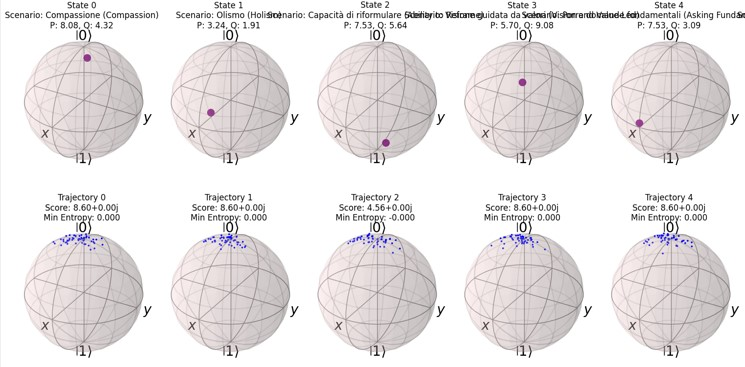
\includegraphics[width=0.9\linewidth]{images/quantuLeadershipNN(1).jpg}
\caption{A Visual Representation of RQM Trajectories.}
\label{fig:trajectories}
\end{figure}

The images show a project's journey through its "pilot wave," which is the wave of all possible scenarios. The spheres are known as Bloch Spheres, a tool from quantum mechanics used to visualize the state of a quantum system. In this context, they represent the state of a project at different moments in time.
\subsubsection*{Top Row: The Ideal Trajectory}
Each Bloch sphere and each Bloch vector represents a project state, with its own priority (P) and quality (Q) scores. The single purple dot on each sphere is the abstract phase of project that would take if there were no biases or noise. 

\subsubsection*{Bottom Row: The Real-World Trajectory}
The bottom row shows a more realistic picture. The single purple dot is gone, replaced by a cluster of blue dots. These dots represent all the possible paths or decisions the project could take at that moment. The spread of the dots visually represents the total uncertainty ($\sigma_{total}$), which is a combination of bias and noise.
\begin{itemize}
\item \textbf{Bias}: If the entire cluster of blue dots were systematically off-center from the ideal path, that would represent a project with a high degree of bias.
\item \textbf{Noise}: The wide spread of the blue dots indicates high noise. This means a team's decisions are inconsistent and unpredictable. A tight cluster of blue dots, even if slightly off-center, would show a more consistent but biased process.
\end{itemize}
The overall goal of RQM is to manage this cluster. A Quantum Manager doesn't try to force the team to hit the single purple dot of the ideal trajectory. Instead, they work to reduce the spread of the blue dots and guide the cluster as a whole towards the ideal path.


The RQM framework uses a neural network to analyze all these possible trajectories and calculate an overall score. A high-scoring trajectory is one with low bias and low noise. The leader's role is to create the environment-through the 12 principles of quantum leadership-that makes a low-uncertainty trajectory the most probable one. For instance, humility and self-awareness would reduce bias, while spontaneity and celebrating diversity would combat noise. The images show a project's pilot wave over time. You can see how the clusters of dots start to spread out, showing increasing uncertainty as the project evolves. The relativistic quantum leader accepts this ambiguity and uses tools and principles to guide the wave. The project's final state is not predetermined; it is the outcome that is most probable due to the leader's management of the system. The model helps them predict which of these many possibilities will most likely lead to a successful "collapse" of the wave into a finished project.
\newpage
\section{ESG Principles \& Asset Management within Relativistic Quantum Management Framework}
$$E(r_{i})=r_{f}+\beta_{i}(E(r_{m})-r_{f}) \quad \beta_{i}=\frac{cov(r_{i},r_{m})}{var(r_{m})}$$
\begin{comment}
\begin{itemize}
    \item La matematica della frontiera di portafoglio (Markowitz)
    \item valore atteso e varianza dei rendimenti
    \item effetto diversificazione e diversificazione naive
    \item frontiera efficiente con 2 asset rischiosi e con un riskless asset
    \item scelta di portafoglio
    \item capital market line (CML)
    \item security market line (SML) e CAPM
    \item APPENDICE frontiera efficiente con n asset
\end{itemize}
\end{comment}

Let's assume that investors only consider the mean and variance of portfolio returns, preferring higher values for the former and lower values for the latter \cite{elisaluciano}.

The portfolio return ($R_p$) is given by:
$$R_{p}=\alpha_{1}r_{1}+\alpha_{2}r_{2}+....+\alpha_{n}r_{n}=\sum_{i=1}^{n}\alpha_{i}r_{i}$$

The expected portfolio return ($E(R_p)$):
$$E(R_{p}) = \sum_{i=1}^{n}\alpha_{i}E(r_{i})$$

The portfolio return variance ($var(R_p)$):
$$var(R_{p}) = \sum_{i=1}^{n}\alpha_{i}^{2}var(r_{i})+\sum_{i=1}^{n}\sum_{j\ne i}\alpha_{i}\alpha_{j}covar(r_{i},r_{j})$$
$$ \sigma^{2}=\sum_{i=1}^{n}\sum_{j=1}^{n}\alpha_{i}\alpha_{j}\sigma_{i}\sigma_{j}\rho_{ij} $$

\begin{itemize}
    \item Covariance Matrix (hypothesized as R):
    $$R=\begin{bmatrix}1 & \dots & \rho_{1m} & \dots \\ \rho_{21} & 1 & \dots & \dots \\ \vdots & \vdots & \ddots & \dots \\ \rho_{n1} & \dots & \dots & 1\end{bmatrix}$$
    (Note: The matrix $R$ is not fully defined, but it appears to represent correlations or a general covariance structure. The full matrix is incomplete.)

    \item Diagonal Matrix of Standard Deviations ($\mathcal{S}$):
    $$\mathcal{S}=\begin{bmatrix}\sigma_{1} & 0 & \dots \\ 0 & \sigma_{2} & \dots \\ \vdots & \vdots & \ddots \end{bmatrix}$$

    \item Vector of Weights ($\alpha$):
    $$\alpha=\begin{bmatrix}\alpha_{1}\\ \alpha_{2}\\ \vdots \\ \alpha_{n}\end{bmatrix}$$
    
    \item Variance Formula in Matrix Notation:
    $$\sigma^{2}=\alpha^{T}S R S^{T}\alpha$$
\end{itemize}
The traditional model can be reviewed in a Relativistic Quantum Management Optic considering the process of forecasting of an asset.
In particular, this is related to the market behavior which is based on some factors such as 
\begin{itemize}
    \item \textbf{Psychological Factors}:
    Motivation, perception, learning, attitudes, and beliefs drive consumer choices and reactions to marketing messages.
    \item \textbf{Personal Factors}:
An individual's age, income, occupation, and lifestyle play a crucial role in determining their needs and purchasing power. 
    \item \textbf{Cultural Factors}:
Beliefs, values, customs, and traditions within a particular community or society shape consumer needs and behaviors. 
    \item \textbf{Social Factors}:
A person's family, reference groups (friends, colleagues), social status, and roles within communities influence their buying habits. 
    \item \textbf{Economic Factors}:
    Conditions like income levels, credit availability, and overall economic stability significantly impact consumer spending and market dynamics. 
    \item \textbf{Technological Factors}:
Advances in technology influence how products are made, marketed, and purchased, leading to new behaviors and opportunities. 
    \item \textbf{Political and Legal Factors}:
Laws, government regulations, and political stability influence market operations and consumer trust. 
    \item \textbf{Environmental Factors}:
Broader shifts in demographics, environmental concerns, and global trends create changing landscapes for businesses and consumers. 
\end{itemize}
Businesses analyze these factors, often using models like PESTLE analysis, to understand how their target audience makes purchasing decisions. By adapting to evolving consumer expectations and market shifts, companies can develop more effective strategies to reach and engage their customers.

A first point could be to rewrite the variance depending also on the variance ($\delta_i$) of these factors thus to account other factors, in the most general way:
\begin{itemize}
    \item covariance matrix
    $$R\prime=\begin{bmatrix}1 & \dots & \rho\prime_{1m} & \dots \\ \rho\prime_{21} & 1 & \dots & \dots \\ \vdots & \vdots & \ddots & \dots \\ \rho\prime_{n1} & \dots & \dots & 1\end{bmatrix}$$

    \item standard deviation ($\mathcal{S}$):
    $$\mathcal{D}=\begin{bmatrix}\delta_{1} & 0 & \dots \\ 0 & \delta_{2} & \dots \\ \vdots & \vdots & \ddots \end{bmatrix}$$

    \item weights ($\alpha\prime$):
    $$\alpha\prime=\begin{bmatrix}\alpha\prime_{1}\\ \alpha\prime_{2}\\ \vdots \\ \alpha\prime_{n}\end{bmatrix}$$
    
    \item variance:
    $$\sigma^{2}=\alpha^{T}S R S^{T}\alpha + \alpha\prime^T D R\prime D^T \alpha\prime$$
\end{itemize}

The extension of this to the relativistic quantum management framework could be in rewriting the entropy and the action of the pilot wave as follows:
\begin{equation}
    \psi_{r_m} = e^{iS_{r_i}}
\end{equation}
where $S_{r_i}$ is the phase of the pilot global wave, the market.
I then define a velocity of the market
\begin{equation}
   v_{market} =  \frac{dq}{dt} =  \nabla{S_{r_i}(t, x)} \cdot {\text{Factors Market Behaviour}}
\end{equation}
where the gradient depend on the time t and on the space x. q(t) is the trajectory.
The diffusion of the wave is as follows
\begin{equation}
    J = \frac{d \rho_{r_i}}{dt}
\end{equation}
It is inspired by Fick's law.

Indeed, the entropy of the whole ensemble, in a given time, would be given by
\begin{equation}
    dS_{r_m} = \sum_i (d\rho_{r_i} \cdot p_i) t
\end{equation}\\
\begin{equation}
    \frac{\partial S}{\partial \rho_{r_i}} = p_i t
\end{equation}
where the evolution of the mixture state is given by Von-Neumann, inspired by Liouville:
\begin{equation}
    d\rho_{r_i} = \frac{\partial{\rho_{r_i}}}{\partial t} + \{H, \rho_{r_i}\} =0
\end{equation}
The clue is to get $S = 0$.
The total energies would respect the statistics as follows:
\begin{equation}
    A = U - TS (V,T const)
\end{equation}
\begin{equation}
    G = H - TS (P, T const)
\end{equation}
where T is the temperature, S is the entropy, H is the entalpy and G is the Gibbs energy.
\\\\
The RQM framework extends this model by introducing a new term to the variance equation to account for these external factors:
\begin{equation}
\sigma^{2}=\alpha^{T}S R S^{T}\alpha + \alpha\prime^T D R\prime D^T \alpha\prime
\end{equation}
\begin{itemize}
\item The first term ($\alpha^{T}S R S^{T}\alpha$) represents the risk from the assets themselves.
\item The second term ($\alpha^{\prime T}DR^\prime D^T \alpha^\prime$) is the key addition. It quantifies the risk introduced by the external market factors.
\end{itemize}
This new formulation suggests that a portfolio's total risk is not just about the assets within it, but also about the unpredictable, dynamic environment in which it exists.

\subsubsection*{The Quantum Market: A Sea of Possibilities}
To manage this complexity, RQM uses concepts from quantum mechanics to model the market's behavior.
\begin{itemize}
\item \textbf{The Market as a Pilot Wave}: In this view, the market is not a single, predictable line. It is a global pilot wave that carries all possible future scenarios. The phase ($S_{r_i}$) of this wave represents its current state and evolution.
\item \textbf{Market Velocity ($v_{market}$)}: The speed at which the market "moves" is determined by its inherent state and the influence of all those external factors.
\item \textbf{Market Diffusion (J)}: This describes how a change in one part of the market spreads or diffuses through the whole system.
\end{itemize}
The entropy ($S_{r_m}$) of the market measures its level of disorder. A highly entropic, or chaotic, market is hard to predict. The goal of a leader is to make decisions that minimize this entropy, bringing the system to a more stable state (S=0).

\subsubsection*{The Propagator and Realism: Predicting the Future}
The final and most powerful idea is the use of the Path Integral, also called the $\phi \epsilon \rho \omega$ (phero) propagator. This is the ultimate forecasting tool in the RQM framework.
\begin{equation}
\phi\epsilon\rho\omega(q_b, t_b; q_a, t_a) = \int_{q(t_a)=q_a; q(t_b)=q_b} \mathcal{D}^f \text{scenario}(\cdot) e^{\frac{i}{\text{realism}} S_{r_i}}
\end{equation}
\begin{itemize}
\item \textbf{The Propagator ($\phi \epsilon \rho \omega$)}: This represents the overall probability of the market moving from its current state (qa) to a desired future state (qb).
\item \textbf{The Integral ($\int Dfscenario())$}: This is a sum over all possible scenarios the market could take. Instead of trying to find the one correct forecast, this framework acknowledges that many futures are possible.
\item \textbf{The "Weighting" Factor ($e^{\frac{i}{realism} S_{r_i}}
$)}: This is what gives the model its power. It assigns a "score" or weight to each possible scenario based on its realism. This new "quantum factor" represents the leader's ability to ground their decisions in the reality of the market, accounting for all its complexities, biases, and noises.
\end{itemize}
By using this model, a leader can make decisions by considering a multitude of realistic scenarios, each weighted by its own "realism," thereby increasing the probability of navigating the market successfully. This is a profound shift from trying to predict the future to actively shaping it by making realistic, well-informed decisions.

\subsubsection*{Measuring Realism}
Measuring "realism" requires moving beyond deterministic models to a probabilistic framework that incorporates a wide range of potential market states. Here are some ways to conceptualize and measure it:
 

 
 A high degree of "realism" means a portfolio model considers a more complete set of market scenarios.
 \begin{itemize}
 	\item \textbf{Tail Risk Capture}: "Realism" can be measured by how well a model accounts for extreme, low-probability events (known as "tail risks"). A model with high realism would not just focus on normal market conditions but would also accurately assess the potential impact of Black Swan events, financial crises, or geopolitical shocks.
 	\item \textbf{Distribution Skewness and Kurtosis}: A classical model often assumes a normal (bell-curve) distribution of returns. However, real-world returns often have "fatter tails" and are skewed. "Realism" could be quantified by how well a model's simulated return distribution matches the skewness and kurtosis of actual historical returns.
 	\item \textbf{Number of Scenarios}: A crude but simple metric could be the number of distinct, well-defined scenarios a model considers. The path integral implies an infinite number of scenarios, so a higher number of simulated paths would correspond to higher realism.
 \end{itemize}
 "Realism" is also tied to a model's ability to adapt to new information and changes in market dynamics.
 \begin{itemize}
 	\item \textbf{Parameter Refresh Rate}: The frequency at which a model's underlying parameters (e.g., correlations, volatilities) are updated based on new market data. A higher refresh rate indicates a more realistic and responsive model.
 	\item \textbf{Predictive Accuracy Under Stress}: A key test of a model's realism is its predictive accuracy during periods of high market stress or volatility, when classical models often fail. A model that performs well during a crisis would be considered highly realistic.
 \end{itemize}
 True "realism" should extend beyond quantitative data to include qualitative factors that are difficult to model.
 \begin{itemize}
 	\item \textbf{Qualitative Inclusion Score}: A metric that assesses the extent to which a model incorporates human behavioral factors, regulatory changes, or technological disruptions, which are often overlooked in purely quantitative frameworks.
 	\item \textbf{Decision-Making Alignment}: The degree to which the model's output influences actual management decisions. If the "realistic" model provides a comprehensive view but is ignored in favor of simpler, less-realistic metrics, then its value is not being fully realized.
 \end{itemize}
 
I remind that a good decision depends on the proper use of System 1 and System 2, as explained in Dual Process Theory and in Prospect Theory \ref{dual}. 

A good decision in terms of investment has consequences on the play between risk and return, in active and passive strategies.


In particular, in the case of bond portfolios, two factors play key roles in the framework of risk and return: duration and convexity.
The return on a bond portfolio is the weighted average of the returns of its individual bonds. The total return for a bond comes from two sources: the coupon payments and any change in the bond's price. The primary measure for a single bond's potential return is its Yield to Maturity (YTM), which represents the total return anticipated on a bond if the bond is held until it matures.

The risk of a bond portfolio is not measured by volatility alone, as is common with stocks, but by specific factors that are unique to the bond market. 


To accurately measure and manage interest rate risk, financial professionals rely on Duration and Convexity.

In traditional finance, professionals use Duration and Convexity to measure and manage the risk of a bond's price changing due to fluctuations in interest rates. However, the Relativistic Quantum Management (RQM) framework suggests that these concepts alone aren't enough to fully capture the complexity of real-world markets. It proposes a new approach that accounts for all possible future scenarios, not just small, predictable changes.

\begin{itemize}
\item \textbf{Duration (Dmod)}: This is a measure of a bond's price sensitivity to interest rate changes. When interest rates go up, bond prices go down, and duration tells you by how much. For a portfolio, the duration is simply the weighted average of the individual bonds' durations. The RQM framework extends this by introducing a term from special relativity, $\gamma$, into the duration equations.  The gamma ($\gamma$) term is known, in Physics, as the \textbf{Lorentz factor}, a crucial scaling factor in special relativity that quantifies the effects of time dilation and length contraction. It describes how an object's time and length appear to change when it is in motion relative to a stationary observer.

The formula for gamma is:

$$ \gamma = \frac{1}{\sqrt{1 - \frac{v^2}{c^2}}} $$

where $v$ is the relative velocity between the two observers and $c$ is the speed of light. Since $v$ is always less than $c$, the value of $\gamma$ is always greater than or equal to 1.

For a stationary observer, time appears to slow down for an object moving at a high velocity. This phenomenon is called \textbf{time dilation}. The relationship is given by:

$$ \Delta t' = \gamma \Delta t $$

Here, $\Delta t'$ is the time interval measured by the stationary observer, while $\Delta t$ is the time interval measured in the moving object's own frame of reference (known as the "proper time"). Because $\gamma$ is always greater than or equal to 1, the time measured by the stationary observer ($\Delta t'$) will always be greater than the proper time ($\Delta t$). This means that the moving object's clock appears to tick more slowly.

Similarly, the length of a moving object appears to shrink in the direction of its motion, a phenomenon known as \textbf{length contraction}. The relationship is:

$$ L' = \frac{L}{\gamma} $$

In this equation, $L'$ is the length of the moving object as measured by the stationary observer, and $L$ is the length of the object in its own reference frame (the "proper length"). Since $\gamma$ is always greater than 1, the measured length $L'$ will always be shorter than the proper length $L$. The faster an object moves, the larger the value of $\gamma$ becomes, and the more its length appears to contract.


Analogously, a project's timeline or scope can appear to expand or contract depending on the infomration processing of its execution, much like time and space change from an observer's perspective in physics.
\item \textbf{Convexity}: While duration works well for small changes, the relationship between a bond's price and interest rates is actually a curve. Convexity measures this curvature. A bond with high convexity is more resilient to interest rate increases and benefits more from decreases, making it more desirable. The convexity of a portfolio is the weighted average of the convexities of the bonds within it.
\end{itemize}


Duration is a measure of the sensitivity of a bond's price to changes in interest rates. A higher duration indicates greater price sensitivity. It is an essential tool for bond portfolio management and is used to estimate the percentage change in a bond's price for a 1\% change in its yield.

The most commonly used duration measure is Modified Duration. The formula for the percentage change in a bond's price is approximated as:
\begin{equation}
    \% \nabla P \sim - D_{mod} \cdot \nabla y \rightarrow -D_{mod} \cdot \gamma \cdot \Delta y
\end{equation}
where $\gamma$ is the special relativity inspired term. In particular, the modified duration could be subjected to a contraction of times or to elongation of space similarly as special relativity. 


where:
\begin{itemize}
\item Dmod is the modified duration of the bond: the relationship between bond prices and interest rates is inverse: when interest rates rise, bond prices fall, and vice versa. Modified duration gives you a way to estimate how much a bond's price will change given a specific shift in interest rates. A higher modified duration means the bond's price will be more volatile and sensitive to rate changes. 
\item $\nabla y$ is the change in the bond's yield to maturity.
\end{itemize}

A portfolio's duration is simply the weighted average of the modified durations of the individual bonds in the portfolio:
\begin{equation}
    D_{portfolio} = \sum_{i=1}^n w_i D_{mod,i} \rightarrow \sum_{i=1}^n w_i \cdot \gamma \cdot D_{mod,i}
\end{equation}
Here, the reasoning is similar: given the presence of $\gamma$, the portoflio duration could change along relativity principles.


where:
\begin{itemize}
\item wi is the market value weight of bond i in the portfolio.
\item Dmod,i is the modified duration of bond i.
\end{itemize}


While duration provides a good approximation for small changes in interest rates, the relationship between a bond's price and its yield is not linear; it is a curve. Convexity measures the curvature of this relationship and accounts for the error in the duration approximation. A bond with higher convexity is more desirable because its price increases more when rates fall and decreases less when rates rise, for a given change in yield.

The percentage change in a bond's price, adjusted for convexity, is given by the more accurate formula:
\begin{equation}
    \%\nabla P \sim (- \text{Dmod} \cdot \nabla y) + (\frac{1}{2} \cdot Convexity \cdot (\nabla y)^2)
\end{equation}


The convexity of a bond portfolio is the weighted average of the convexities of the individual bonds:
\begin{equation}
    \text{Convexity Portfolio} = \sum_{i=1}^n w_i Convexity_i
\end{equation}


where:
\begin{itemize}
\item wi is the market value weight of bond i.
\item Convexity is the convexity of bond i.
\end{itemize}

The pivotal point, within relativistic quantum management, is given by considering all possible scenarios and therefore $\phi \epsilon \rho \omega$.
Thus the Convexity Portoflio, within Relativistic Quantum Management, would be replaced by
\begin{align}
\phi\epsilon\rho\omega(q_b, t_b; q_a, t_a) = \int_{q(t_a)=q_a; q(t_b)=q_b} \mathcal{D}^f scneario(\cdot) e^{\frac{1}{\text{realism}} \int_{t_a}^{t_b} dt \mathcal{L}(scenario(t), \dot{scenario}(t))}\\ = \int_{q(t_a)=q_a; q(t_b)=q_b} \mathcal{D}^f scenario(\cdot) e^{\frac{i}{\text{realism}s} S_{r_i}} 
\end{align}
looking for the best possible trajectory that minimizes the uncertainty or looking at all possible trajectories.


 In summary, in this relativistic quantum framework,   "realism"   is a measure of a model's comprehensiveness and its ability to accurately reflect the full complexity and uncertainty of financial markets, including non-linear effects and improbable events.
 

\subsection{How to Make a Good Investment Decision through the Prospect Theory lens}
Prospect theory, developed by Daniel Kahneman and Amos Tversky, describes how people make decisions under uncertainty. It presents a more realistic model than expected utility theory by incorporating cognitive biases like loss aversion. The core of prospect theory is its two main functions: the \textbf{value function} and the \textbf{probability weighting function}.


The value function, $v(x)$, models how people perceive the subjective value of gains and losses. It is defined on deviations from a \textbf{reference point} (e.g., the current wealth). A key feature is its \textbf{S-shape}, which is concave for gains and convex for losses, reflecting diminishing sensitivity. The function is also steeper for losses than for gains, which represents \textbf{loss aversion}.

$$
v(x) =
\begin{cases}
    x^\alpha & \text{if } x \ge 0 \quad (\text{for gains}) \\
    -\lambda (-x)^\beta & \text{if } x < 0 \quad (\text{for losses})
\end{cases}
$$

\begin{itemize}
    \item $x$: The outcome, expressed as a gain ($x>0$) or a loss ($x<0$) relative to the reference point.
    \item $\alpha$: A parameter for gains, typically $0 < \alpha < 1$. The value being less than 1 reflects diminishing sensitivity to gains (e.g., the difference between \$10 and \$20 feels greater than the difference between \$110 and \$120).
    \item $\beta$: A parameter for losses, also typically $0 < \beta < 1$. Similarly, this value reflects diminishing sensitivity to losses.
    \item $\lambda$: The \textbf{coefficient of loss aversion}, which is the most significant parameter. It is usually greater than 1, indicating that the value assigned to a loss is greater in magnitude than the value assigned to an equal-sized gain. Kahneman and Tversky estimated $\lambda \approx 2.25$.
\end{itemize}


The probability weighting function, $\pi(p)$, transforms objective probabilities ($p$) into subjective decision weights ($\pi(p)$). It addresses the observation that people tend to overweight low probabilities and underweight high probabilities. The function is \textbf{inverse-S shaped}, overweighing low probabilities and underweighting high probabilities.

$$
\pi(p) = \frac{p^\gamma}{(p^\gamma + (1-p)^\gamma)^{1/\gamma}}
$$

\begin{itemize}
    \item $p$: The objective probability of an event.
    \item $\gamma$: A parameter that determines the shape of the weighting function, typically $0 < \gamma < 1$. A lower value of $\gamma$ means a more pronounced inverse-S shape (i.e., more extreme overweighting of small probabilities and underweighting of large probabilities). Kahneman and Tversky estimated $\gamma \approx 0.61$ for gains and $0.69$ for losses.
\end{itemize}


The overall value of a prospect (or gamble) is calculated by multiplying the subjective value of each outcome by its corresponding subjective decision weight and summing them up. For a simple prospect with two outcomes, a gain $x$ with probability $p$ and a loss $y$ with probability $1-p$, the prospect value is:

$$
V = \pi(p)v(x) + \pi(1-p)v(y)
$$

For a more general prospect with multiple outcomes:

$$
V = \sum_{i=1}^{n} \pi(p_i)v(x_i)
$$

\begin{itemize}
    \item $V$: The overall prospect value.
    \item $v(x_i)$: The subjective value of outcome $x_i$, as determined by the value function.
    \item $\pi(p_i)$: The subjective decision weight for the probability $p_i$, as determined by the probability weighting function.
\end{itemize}
Traditional economic models, based on Utility Theory, struggle to provide a comprehensive explanation for human behavior in risky situations. The core assumption of a concave utility function—which posits that individuals' satisfaction with wealth increases at a decreasing rate—effectively explains why people are willing to pay a premium for insurance (i.e., they are risk-averse). However, this same principle fails to account for the seemingly contradictory risk-seeking behavior observed when people purchase lottery tickets. To reconcile this paradox, early theories were forced to propose an unwieldy utility function that was concave in some areas and convex in others, a hypothesis that lacked significant empirical support.


The value function describes how individuals subjectively value gains and losses relative to a reference point. This function is notably concave for gains and convex for losses. While this property correctly predicts risk-aversion in the domain of gains and risk-seeking in the domain of losses, it still does not, on its own, fully account for why both insurance and gambling are attractive to consumers.


The key to resolving the paradox lies in uncertainty weights $(\pi(p))$. This concept recognizes that people do not process probabilities linearly. Instead, individuals tend to overweight small probabilities $(\pi(p)>p)$ and underweight outcomes that are probable but not certain.

The allure of both insurance and lotteries stems from a shared feature: they both involve a small probability of a large outcome.
\begin{itemize}
\item In the case of a lottery, the small probability of a large gain is overweighted, which increases the perceived value of the ticket beyond its actual expected value.
\item With insurance, the small probability of a catastrophic loss is overweighted, making the potential uninsured loss appear far more aversive than it is from a purely rational standpoint.
\end{itemize}


Traditional economic theory has long been predicated on the existence of a perfectly rational agent, the "Homo Economicus" or "Econ." This idealized individual is assumed to make decisions by maximizing expected utility, is immune to cognitive biases, and does not change their mind. In stark contrast, behavioral economics and psychology present a different reality: that of the "Human." Humans are guided by intuition, emotions, and mental shortcuts (heuristics) that often lead to choices that deviate from perfect rationality.

Expected Utility Theory serves as the normative model for rational choice, asserting that individuals evaluate risky options by calculating the weighted average of the outcomes' utilities. However, this theory is plagued by empirical anomalies, such as the St. Petersburg Paradox, which revealed that the marginal utility of wealth tends to diminish. While this observation was correctly intuited by Bernoulli, his model's flaw was its assumption that individuals' decisions are based on their final wealth rather than changes in wealth from a reference point.

A variety of biases and cognitive illusions influence decisions, often operating outside conscious awareness.
\subsubsection*{Regression to the Mean}
This bias leads people to ignore the statistical fact that extreme outcomes (both positive and negative) are likely to be followed by more average results. For example, an exceptionally good performance by a company is more likely to be followed by a less stellar one, not because of a flaw, but due to a statistical regression toward the mean.

\subsubsection*{Overconfidence}
Overconfidence is an endemic bias, especially among experts. People tend to overestimate their judgmental abilities and the accuracy of their forecasts. This bias is particularly dangerous when combined with a disregard for competition, as it leads to ignoring the strategic actions of others in a market.

\subsubsection*{Illusion of Validity}
This bias occurs when an individual places unwarranted confidence in their intuitions (System 1), even when evidence is limited. Subjective confidence is not a reliable indicator of accuracy but is a sensation generated by cognitive fluency.

\subsubsection*{Alone Effect (or Isolation Effect)}
Related to the Allais Paradox, the isolation effect describes a tendency for decision-makers to ignore components common to different options and focus solely on what differentiates them. This can lead to inconsistent and seemingly irrational choices.

\subsubsection*{Anchor Effect}
The anchoring effect occurs when an estimate is disproportionately influenced by an initial, often irrelevant, piece of information (the anchor). It is a powerful bias used by negotiators and marketers to influence judgments.

\subsubsection*{Illusion of Financial Ability}
This is a specific form of overconfidence where people mistakenly believe that skill and experience are the primary determinants of success in financial markets, while underestimating the role of chance or luck.

\subsubsection*{Pre-Mortem}
The pre-mortem is a technique proposed by Gary Klein to combat group overconfidence. Before a major decision, the team imagines that a disaster has occurred one year into the future and identifies all the reasons why it might have happened. This technique legitimizes doubt and encourages critical thinking, counteracting groupthink and irrational optimism.

The role of optimism is another central theme. Excessive optimism and false confidence lead to taking on excessive risks. Disregard for competition and wishful thinking are cognitive biases that reinforce this tendency, causing individuals to focus on what they wish would happen rather than what is likely to occur.\\\\\\\\
In conclusion, according to Kahneman's Theory, good decisions could be made by recognizing:
\begin{itemize}
\item \textbf{Reference Dependence}: People evaluate outcomes as gains or losses relative to a neutral reference point (e.g., their current state), not based on their final wealth. Reactions to changes are far stronger than reactions to absolute wealth levels.
\item \textbf{Loss Aversion}: People are significantly more sensitive to losses than to equivalent gains. The displeasure of a loss is roughly 1.5-2.5 times greater than the pleasure of an equivalent gain. This bias explains the disposition effect, where investors are inclined to sell winning stocks too early to secure a gain while holding on to losing stocks for too long in the hope of recovery.
\item \textbf{Probability Weighting}: Individuals tend to overweight small probabilities and underweight moderate to high probabilities. This explains the popularity of both lotteries (overweighting a small chance of a large win) and insurance (overweighting a small chance of a catastrophic loss).
\end{itemize}
There is also to mention that the psychophysical principle of diminishing sensitivity, which states that the impact of a change (e.g., in wealth) lessens as its distance from the reference point increases, akin to a logarithmic function. This function, indeed, is used to describe the efficiency of our senses: there is a growing sentivity till it reaches a plateau; A practical example is what happens when we smell something bad, after some time, we will get used to it.


\newpage
\subsection{Simulation of Asset Management with $\phi$QINN}

\begin{figure}[!ht]
\centering
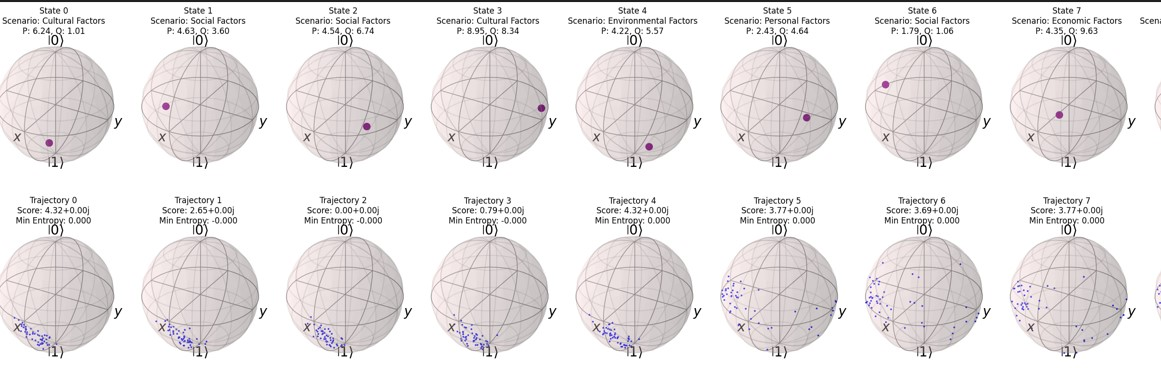
\includegraphics[width=0.9\linewidth]{images/assetManag.jpg}
\caption{A Visual Representation of RQM Trajectories.}
\label{fig:trajectoriesass}
\end{figure}

\subsubsection*{Top Row: The Ideal Trajectory}
The top row of the images shows an ideal or reference trajectory for a project. Each sphere represents a project state, with its own space (x) and time (t) of an asset. The asset management is here defined in terms of market factors that could influence the decision.
In particular, the Bloch vector is associated to a particular phase of the factor, without considering uncertainty. 

\subsubsection*{Bottom Row: The Real-World Trajectory}
The bottom row shows a more realistic picture. The single purple dot is gone, replaced by a cluster of blue dots. These dots represent all the possible paths or decisions the project could take at that moment. The spread of the dots visually represents the total uncertainty ($\sigma_{total}$), which is a combination of bias and noise.
\begin{itemize}
\item \textbf{Bias}: If the entire cluster of blue dots were systematically off-center from the ideal path, that would represent a project with a high degree of bias.
\item \textbf{Noise}: The wide spread of the blue dots indicates high noise. This means a team's decisions are inconsistent and unpredictable. A tight cluster of blue dots, even if slightly off-center, would show a more consistent but biased process.
\end{itemize}


\begin{itemize}
\item \textbf{Fostering Realism}: The RQM framework uses a neural network to analyze all these possible trajectories and calculate an overall score. A high-scoring trajectory is one with low bias and low noise. The leader's role is to make a good asset management decision that makes a low-entropy trajectory the most probable one. 
\item \textbf{From Possibility to Outcome}: The images show a project's pilot wave over time. You can see how the clusters of dots start to spread out, showing increasing uncertainty as the project evolves. The relativistic quantum leader accepts this ambiguity and uses tools and principles to guide the wave. The project's final state is not predetermined; it is the outcome that is most probable due to the leader's management of the system. The model helps them predict which of these many possibilities will most likely lead to a successful "collapse" of the wave into a finished project.
\end{itemize}
\newpage
\section{ESG Principles \& IOT within Relativistic Quantum Management Framework}
\label{Sec5}
\subsection*{Environmental, Social and Governance Principles}
The \textbf{ESG} framework is a set of principles used to evaluate an organization's performance across three key areas: \textbf{Environmental}, \textbf{Social}, and \textbf{Governance}. It serves as a vital tool for investors, customers, and employees who seek to understand a company's commitment to ethical and sustainable practices beyond its financial metrics.


This pillar assesses a company's impact on the natural world and its role as a steward of the environment. Key considerations include:

\begin{itemize}
    \item \textbf{Climate Change and Carbon Footprint}: A company's efforts to reduce greenhouse gas emissions and transition to renewable energy sources.
    \item \textbf{Pollution and Waste Management}: Policies and actions for handling waste, minimizing air and water pollution, and promoting resource efficiency.
    \item \textbf{Natural Resource Conservation}: The approach to using and conserving natural resources like water and raw materials sustainably.
    \item \textbf{Biodiversity}: Efforts to protect and restore ecosystems affected by business operations.
\end{itemize}


The social pillar examines how a company manages its relationships with stakeholders, including employees, customers, suppliers, and the broader community. It focuses on ethical and responsible behavior. Key considerations include:

\begin{itemize}
    \item \textbf{Labor Practices and Human Rights}: Ensuring fair wages, safe working conditions, and ethical labor practices throughout the supply chain.
    \item \textbf{Diversity, Equity, and Inclusion (DEI)}: Promoting a diverse workforce, ensuring equal opportunities, and fostering an inclusive culture.
    \item \textbf{Customer and Community Relations}: The company's commitment to consumer protection, product safety, data privacy, and positive community engagement.
    \item \textbf{Employee Health and Safety}: Practices that prioritize the well-being and safety of all employees.
\end{itemize}

This pillar refers to the internal system of practices and controls a company uses for effective management, decision-making, and legal compliance. It ensures accountability and transparency. Key considerations include:

\begin{itemize}
    \item \textbf{Board Structure and Diversity}: The independence, effectiveness, and diversity of the company's board of directors.
    \item \textbf{Executive Compensation}: How executive pay is structured and whether it aligns with the company's long-term performance and values.
    \item \textbf{Shareholder Rights}: Ensuring fair treatment and a voice for all shareholders in major company decisions.
    \item \textbf{Ethics and Transparency}: The implementation of anti-corruption policies, ethical business practices, and clear financial reporting.
\end{itemize}


Integrating ESG principles helps companies to:
\begin{itemize}
    \item \textbf{Mitigate Risks}: Proactively manage non-financial risks that could affect long-term value.
    \item \textbf{Attract Investment}: Appeal to a growing number of investors who use ESG criteria to screen for resilient and stable companies.
    \item \textbf{Enhance Reputation}: Build trust with customers, employees, and the public, leading to increased brand loyalty.
    \item \textbf{Improve Performance}: Drive operational efficiencies and boost employee morale, leading to improved productivity and innovation.
\end{itemize}
\subsection*{Internet of Things}
The \textbf{Internet of Things (IoT)} is a network of physical objects that are embedded with sensors, software, and other technologies to connect and exchange data with other devices and systems over the internet. Essentially, it extends internet connectivity beyond standard devices like computers and smartphones to a wide range of everyday things.

An IoT system typically operates in a few key steps:

\begin{enumerate}
    \item \textbf{Sensors and Devices}: These devices collect data from their environment. For example, a smart thermostat measures temperature, or a sensor in a car's engine measures oil pressure.
    \item \textbf{Connectivity}: The collected data is sent to a central hub or cloud-based platform using various forms of connectivity such as Wi-Fi, Bluetooth, cellular networks, or satellite links.
    \item \textbf{Data Processing}: Once in the cloud, software processes and analyzes the data. Algorithms can detect patterns, identify anomalies, or make predictions.
    \item \textbf{User Interface}: The processed information is made available to the user through a dashboard, mobile app, or a notification. Users can also send commands back to the devices, like adjusting the temperature from their phone.
\end{enumerate}

IoT is becoming increasingly integrated into our daily lives, with common examples including:

\begin{itemize}
    \item \textbf{Smart Homes}: Devices like smart speakers, connected lights, and security systems that can be controlled remotely.
    \item \textbf{Wearables}: Fitness trackers and smartwatches that monitor health data like heart rate and steps.
    \item \textbf{Connected Cars}: Vehicles with sensors that monitor engine performance, fuel levels, and offer remote diagnostics.
    \item \textbf{Industrial IoT (IIoT)}: In manufacturing, sensors on factory machines can monitor their performance to predict maintenance needs and improve efficiency.
\end{itemize}

The main benefits of IoT are increased \textbf{efficiency}, \textbf{convenience}, and the ability to gather valuable data for better decision-making. However, IoT also presents significant challenges, particularly regarding \textbf{security} and \textbf{privacy}. The vast network of connected devices creates a larger surface for cyberattacks, and the constant collection of personal data raises concerns about who owns and has access to this information.\\\\\\
The $\phi QINN$ neural network's ability to predict a quality score by implicitly accounting for bias and noise is the essence of RQM. This framework, inspired by quantum mechanics, views a project's future not as a single, certain path but as a wave of possibilities. The leader's role is to guide this wave towards a desired outcome by minimizing uncertainty.

By learning to predict the score S, the model provides a quantitative tool for leaders. It helps them understand which factors and paths are most likely to lead to a successful outcome, allowing them to make data-driven decisions that actively reduce the impact of bias and noise. The model, in a sense, provides a "quantum forecast," enabling leaders to navigate a complex, uncertain landscape more effectively.

The foundation of this approach is quantum information theory, which uses quantum principles like superposition and entanglement to perform complex calculations. While classical computers use bits (0s or 1s), quantum computers use qubits, which can be both 0 and 1 at the same time. This power is essential for the RQM framework, as it allows us to model a system's uncertainty and the multitude of possibilities that exist simultaneously.

In this section, it is applied to an ESG IoT platform, a system that collects data on environmental, social, and governance factors. The platform is designed to:
\begin{itemize}
\item \textbf{Monitor Environmental Data}: It tracks things like $CO_2$ emissions and waste.
\item \textbf{Analyze Social Factors}: It uses tools like Large Language Models (LLMs) for sentiment analysis to understand public opinion.
\item \textbf{Assess Governance}: It processes financial reports to evaluate a company's leadership and stability.
\end{itemize}
A RQM perspective treats this entire ESG system as a single, interconnected entity.

To manage this complex system, RQM uses a mathematical formalism inspired by quantum mechanics.
\begin{equation}
    \psi_{balance_{ESG}} = e^{iS_{E}, S_{G}, S_{S}}
\end{equation}
where $S_{r_i}$ is the phase of the pilot global wave, the market.
I then define a velocity of the market
\begin{equation}
   v_{balance_{ESG}} =  \frac{dq}{dt} =  \nabla{S_{E}(x, t)} \cdot {\text{Factors Environment}} + \nabla{S_{G}(x, t)} \cdot {\text{Factors Governance}} + \nabla{S_{S}(x, t)} \cdot {\text{Factors Social}}
\end{equation}
where the gradient depend on the time t and on the space x. q(t) is the trajectory.
The diffusion of the wave is as follows
\begin{equation}
    J = \frac{d \rho_{S_E}}{dt} + \frac{d \rho_{S_G}}{dt} + \frac{d \rho_{S_S}}{dt}
\end{equation}
It is inspired by Fick's law.

Indeed, the entropy of the whole ensemble, in a given time, would be given by
\begin{equation}
    dS_{balance_{ESG}} = \sum_i (d\rho_{r_{E,S,G}} \cdot p_{E,S,G}) t
\end{equation}\\
\begin{equation}
    \frac{\partial S}{\partial \rho_{r_{E,S,G,}}} = p_{E,S,G} t
\end{equation}
where the evolution of the mixture state is given by Von-Neumann, inspired by Liouville:
\begin{equation}
    d\rho_{r_{E,S,G}} = \frac{\partial{\rho_{r_{E,S,G}}}}{\partial t} + \{H, \rho_{r_{E,S,G}}\} =0
\end{equation}
The clue is to get $S = 0$.
The total energies would respect the statistics as follows:
\begin{equation}
    A = U - TS (V,T const)
\end{equation}
\begin{equation}
    G = H - TS (P, T const)
\end{equation}
where T is the temperature, S is the entropy, H is the Entalpy and G is the Gibbs energy.
\begin{equation}
\phi\epsilon\rho\omega(q_b, t_b; q_a, t_a) = \int_{q(t_a)=q_a; q(t_b)=q_b} \mathcal{D}^f \text{scenario}(\cdot) e^{\frac{i}{\text{balance}} S_{r_{E,S,G}}}
\end{equation}
\begin{itemize}
\item \textbf{The Global Pilot Wave ($\psi_{balanceESG}$)}: This is the central concept. It represents the overall balance of the entire ESG system. Instead of focusing on individual metrics, the leader manages this wave, which contains all possible future states of the ESG balance.
\item \textbf{Trajectory}: The movement of this wave is defined by the global balance among the ESG principles. It depends on a gradient in a phase-space scenario, meaning that the direction and speed of the system's evolution are influenced by the interactions between all of its components.
\item \textbf{Diffusion}: This concept describes how a change in one part of the system affects the others. For instance, a change in a company's social policy (a local principle) will "diffuse" and affect its environmental and governance standing. This diffusion is governed by an equation that models the spread of change throughout the system.
\item \textbf{Entropy}: The entropy of the system measures its level of disorder or imbalance. The goal of a quantum leader is to drive the system towards a state of minimum entropy (S=0), which represents a state of perfect balance and stability. This is the ideal state where the ESG factors are in harmony, and the system is predictable and resilient.
\end{itemize}

\subsubsection*{Measuring Balance}
Measuring balance in an ESG (Environmental, Social, and Governance) context through Quantum Management involves shifting from a rigid, classical approach to a dynamic, holistic one that embraces uncertainty and interconnectedness. This model views a company's ESG performance not as a static score but as a complex, evolving state.

Traditional ESG measurement often relies on a linear, "classical" framework. It uses a series of fixed metrics to generate a single score. The problem is, this approach is ill-suited for the dynamic nature of ESG, where a positive action in one area (e.g., a large-scale environmental investment) might inadvertently create a negative outcome in another (e.g., a social issue with the supply chain). There's no true "balance" because the system's parts are treated as isolated variables rather than as an interconnected whole.

Quantum Management reframes ESG balance as a \textbf{density mixture state}, which is a blend of all possible outcomes. This moves beyond a simple, binary score to a probabilistic model that captures the full spectrum of a company's performance.

\begin{enumerate}
    \item \textbf{Representing ESG as a Bloch Vector:} A company's overall ESG state can be visualized as a \textbf{Bloch vector} within a specialized Bloch sphere. Instead of a quantum particle's "spin up/spin down," the two poles could represent extreme, opposing states: a perfect ESG performer at one pole and a complete laggard at the other.
    \item \textbf{Quantifying Uncertainty:} The length of the Bloch vector measures the company's "purity" or certainty in its ESG performance.
    \begin{itemize}
        \item A vector on the \textbf{surface} of the sphere indicates a highly transparent, well-documented ESG profile with minimal uncertainty.
        \item A vector pointing to the \textbf{center} of the sphere indicates a state of maximum uncertainty, where there is a 50/50 probability of the company being a leader or a laggard in any given ESG metric.
    \end{itemize}
    \item \textbf{Measuring Balance as a the phase:} The true measure of balance is not a single score but rather the \textbf{phase}---a tool that describes the flow of information and influence between the E, S, and G pillars.
    \begin{itemize}
        \item A balanced ESG system would show strong \textbf{entanglement} between the pillars. For example, a successful waste reduction program (Environmental) should lead to improved community relations (Social) and streamlined governance (Governance). The propagator would quantify the strength and direction of these interdependencies.
        \item Conversely, an imbalanced system would show weak or negative propagation, where a positive action in one area fails to positively influence others. This reveals a fragmented approach rather than a cohesive one.
    \end{itemize}
\end{enumerate}
By using quantum computing, leaders can perform the complex calculations needed to model this system and make proactive decisions to maintain balance and minimize uncertainty, rather than simply reacting to problems after they occur.

\begin{figure}[!h]
\centering
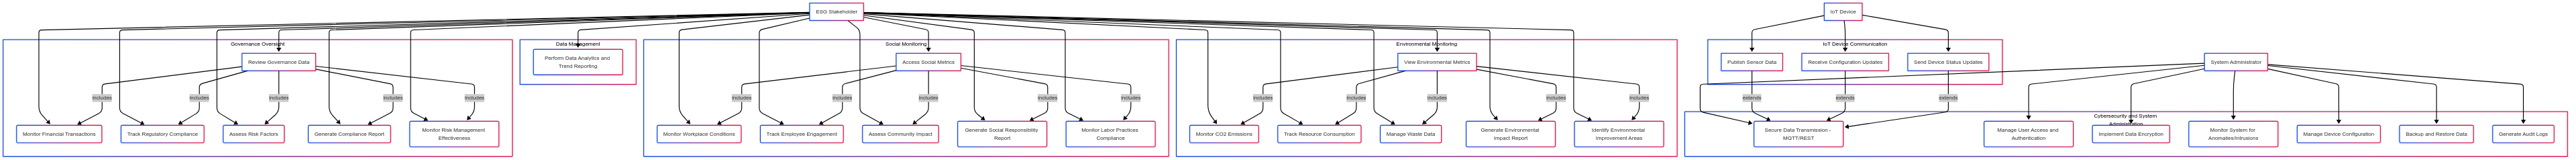
\includegraphics[width=0.9\linewidth]{images/Editor _ Mermaid Chart-2025-06-08-142532(3)(1).png}
\caption{Diagram of Use Case}
\end{figure}

\begin{figure}[!h]
\centering
\begin{subfigure}[b]{0.45\linewidth}
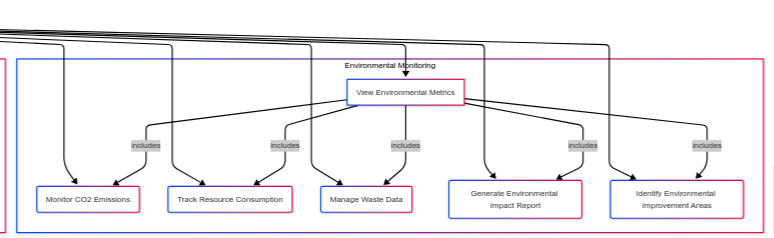
\includegraphics[width=\linewidth]{images/environmentIOT(1).PNG}
\caption{Environment}
\end{subfigure}
\begin{subfigure}[b]{0.45\linewidth}
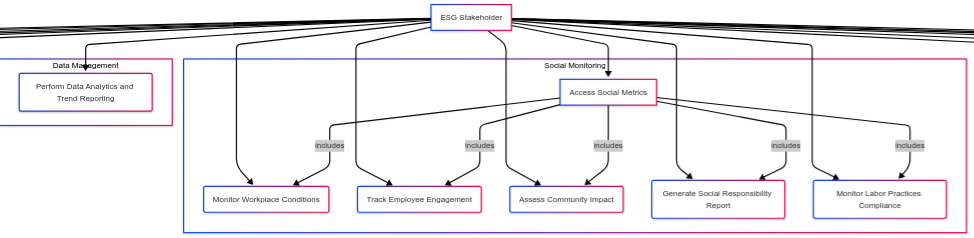
\includegraphics[width=\linewidth]{images/SOCIALiot(1).PNG}
\caption{Social}
\end{subfigure}
\begin{subfigure}[b]{0.45\linewidth}
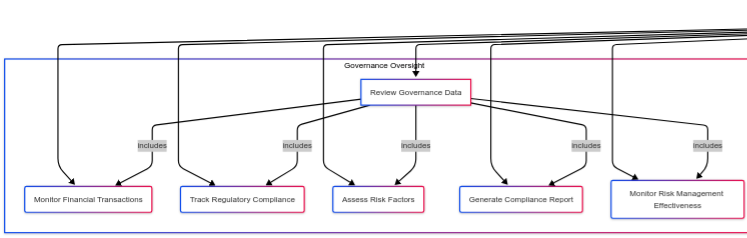
\includegraphics[width=\linewidth]{images/governanceIOT(1).PNG}
\caption{Governance}
\end{subfigure}
\begin{subfigure}[b]{0.45\linewidth}
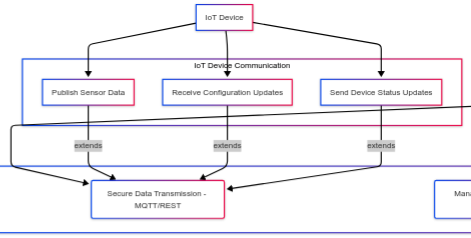
\includegraphics[width=\linewidth]{images/iotcommun(1).PNG}
\caption{Communication}
\end{subfigure}
\begin{subfigure}[b]{0.45\linewidth}
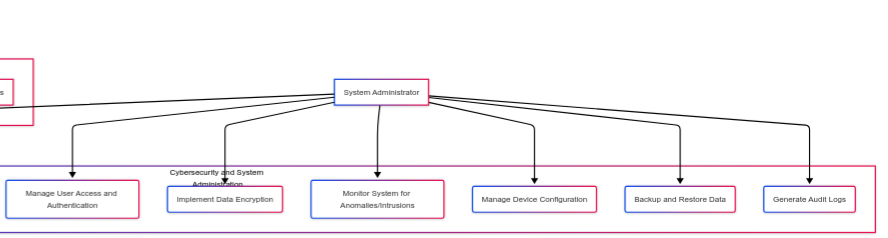
\includegraphics[width=\linewidth]{images/administratorIOT.PNG}
\caption{Administration}
\end{subfigure}
\end{figure}
\newpage
\subsection{Simulation of ESG and IOT with $\phi QINN$}
A simulation using a $\phi$QINN (Quantum Neural Network) models the behavior of the ESG IoT platform. It demonstrates how such a quantum-inspired model can capture the complex, non-linear interactions between environmental, social, and governance factors.

\begin{figure}[!h]
\centering

\includegraphics[width=\linewidth]{images/esg(2).png}
\caption{Simulation of IoT and ESG principles}
\end{figure}

\begin{figure}[!h]
\centering
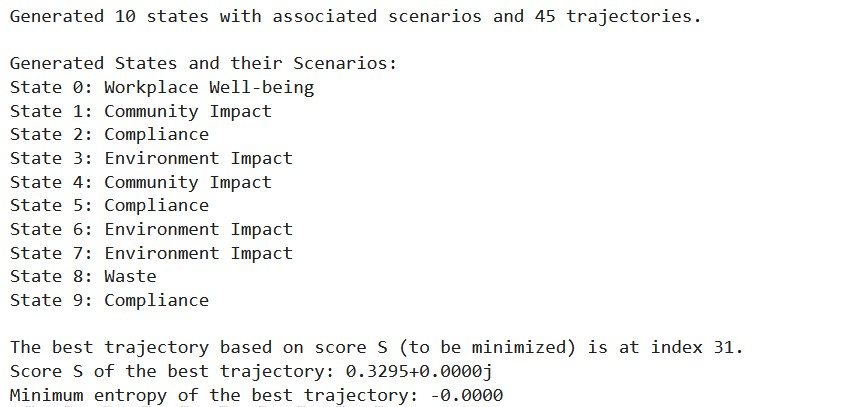
\includegraphics[width=\linewidth]{images/esgPrint(1).jpg}
\caption{Simulation Results}
\end{figure}

The images display a visual metaphor for project management using Bloch Spheres, a concept from quantum mechanics. The top rows represent the ideal, deterministic path of a project. 

The bottom rows, however, show the reality of management in RQM. The single purple dot is replaced by a cluster of blue dots, representing a superposition of all possible project states. This is the project's "pilot wave," containing every potential trajectory it could take. A quantum leader's job isn't to force the project onto the ideal purple dot, but to manage this entire wave.
\begin{itemize}
\item The spread of the blue dots visualizes the project's total uncertainty ($\sigma_{total}$). A wide, dispersed cluster indicates high noise ($\sigma_{noise}$) or inconsistency in decision-making. If the entire cluster is off-center from the ideal purple dot, that represents a bias ($\sigma_{bias}$) in the project's path.
\item The neural network and its associated output are the predictive tools that analyze these complex trajectories. They assign a score (S) to each path, with the goal of identifying the best possible trajectory-the one with the lowest score and minimum entropy. The neural network's calculations implicitly account for the bias and noise of each path to determine this score.
\end{itemize}

The second output provides a concrete example of this framework applied to ESG management. It shows that a simulation generated 45 possible trajectories for an ESG project, each influenced by different scenarios like "Workplace Well-being" or "Environment Impact". The goal of the model is to find the best possible trajectory---the one that minimizes the score (S) and entropy.
\begin{itemize}
\item \textbf{Entropy}: In RQM, entropy measures the level of disorder or imbalance in a system. The output shows that the best trajectory (index 31) has a score of 0.3295 and a minimum entropy of 0.0000. This indicates that this specific path is the most stable and predictable, making it the most desirable option for a leader to pursue. The goal of a quantum leader is to make decisions that drive the system towards a state of minimum entropy (S=0), which represents a state of perfect balance and stability.
\item \textbf{The Leader's Role}: The leader uses the output of this model to make proactive, data-driven decisions. Instead of guessing, they can use the neural network's forecast to choose the trajectory with the highest probability of success. They then use the principles of quantum leadership (like fostering a culture of trust and encouraging collaboration) to guide the project's pilot wave along that path, actively minimizing uncertainty and guiding the organization toward a successful outcome.
\end{itemize}

All this relies on a very important and precious resource: \textbf{information}. It is therefore necessary to assure security and protection of it, above all within digital systems.
In this increasingly interconnected world, almost every aspect of life, from personal banking to national infrastructure, relies on digital systems. This reliance creates vulnerabilities that malicious actors—like hackers, cybercriminals, and state-sponsored groups—can exploit. In the next section, I propose a potential system based on topological quantum computing that could be applied in a system (IOT) to protect information.
\newpage
\subsection{Topological Quantum Cybersecurity and Information Processing}
Cybersecurity in IoT systems is crucial for protecting the vast network of connected devices and the data they generate and transmit. It involves safeguarding these devices from unauthorized access, attacks, and exploitation, which could lead to data theft, privacy breaches, and physical harm.
This section explores the use of topological qubits and anyons for cybersecurity within an IoT context, particularly for securing data transmission. The approach combines the mathematical rigor of elliptic curve cryptography with the robust, non-commutative properties of quantum braids.

Topological quantum computing uses quasiparticles called anyons to encode quantum information: instead of relying on the quantum state of a single particle, it stores information in the braiding patterns of these anyons as they move. This topological approach makes the qubits inherently more robust against noise and errors because the information is protected by the global properties of the braid (topological group), not by local, fragile states.

Topological Quantum Cybersecurity is a potential approach to securing data in the age of the Internet of Things (IoT). It combines a familiar concept from classical cryptography, elliptic curves, with the unique, robust properties of quantum braids to create a highly secure system.

\subsubsection*{How Topological Quantum Cybersecurity would work}
Quantum computing leverages the principles of quantum mechanics to perform computations. Unlike classical bits, which can only be 0 or 1, a quantum bit or qubit can exist in a superposition of both states simultaneously. This property, along with entanglement, allows quantum computers to solve certain problems, such as factoring large numbers, exponentially faster than classical computers.

\textit{Quantum information theory} is the study of how \textbf{information} is stored, processed, and transmitted using quantum systems. It deals with concepts like quantum states, quantum gates, and the challenges of decoherence and noise. Decoherence is the loss of quantum properties due to the interaction of a quantum system with its environment. This interaction introduces errors and is a major hurdle in building stable and reliable quantum computers.

Most current quantum computing approaches, such as those using superconducting qubits or trapped ions, rely on local encoding of information. This means the information is stored in the fragile quantum state of a single particle or a small group of particles. These systems are highly susceptible to noise from their environment. A tiny disturbance can cause the qubit to lose its quantum state, leading to a computational error. This is a significant challenge for creating a reliable quantum computer and, by extension, a secure quantum communication system.

Topological quantum computing offers a revolutionary solution to the noise problem by encoding information non-locally. It doesn't store information in individual particles but in the global properties of a system, specifically in the braiding patterns of anyons.
\begin{itemize}
    \item Anyons: Anyons are quasiparticles—emergent excitations in two-dimensional systems that behave like particles but aren't fundamental particles. Unlike fermions or bosons, which have integer or half-integer exchange statistics, anyons have fractional exchange statistics. This means that when two anyons are swapped, their quantum state changes in a way that depends on the path they took, not just their final positions. Their trajectories over time can be represented as a complex braid.

    \item Topological Qubits: In this approach, a qubit's information isn't tied to a single anyon. Instead, it's encoded in the braiding pattern of multiple anyons. To change the state of the qubit, you must physically change the entire braiding pattern. This is the key to its resilience. A local disturbance, like noise affecting a single anyon, can't easily corrupt the encoded information. You'd have to tamper with the entire global structure of the braid, which is incredibly difficult. This property is known as topological protection.

    \item Quantum Operations: Calculations in a topological quantum computer are performed by manipulating and braiding the anyons. These braiding operations correspond to quantum gates. Because the information is protected by the braid's topology, these operations are inherently fault-tolerant and far less susceptible to noise and errors compared to systems that rely on the precise control of fragile local states.
\end{itemize}
By combining the non-local, topologically protected nature of topological qubits with principles from classical cryptography, I propose a new approach to cybersecurity.\\
In a topological quantum cybersecurity system, data could be transmitted by encoding it into the braiding patterns of anyons. A sender could manipulate anyons to create a specific braid that represents the data. The receiver would then "unbraid" the anyons to retrieve the information. Any attempt to eavesdrop or tamper with the transmission would be highly noticeable, as it would likely disrupt the intricate topological structure of the braid, making it impossible to correctly "unbraid" the data. This provides a more secure and fault-tolerant way to protect data from both classical and quantum attacks.
\newpage
In summary
\begin{itemize}
\item \textbf{Anyons}: These are not real particles, but "quasiparticles" in two-dimensional systems with fractional exchange statistics. Their movement can be described as a braid.
\item \textbf{Topological Qubit}: In this approach, information is stored non-locally by braiding anyons. This protects the information from being broken by targeting a single point. You would have to tamper with the entire braiding pattern, which is incredibly difficult.
\item \textbf{Quantum Operations}: Instead of using traditional computing operations, this system performs calculations by braiding the anyons. This method is highly resilient to noise and errors because the information is protected by the global properties of the braid (a topological group), not by local, fragile states.
\end{itemize}
By using these quantum braids and the non-local nature of topological qubits, this approach provides a more robust and fault-tolerant way to secure data transmission, making it a powerful tool for next-generation cybersecurity.
\textbf{Anyons} are quasiparticles in two-dimensional systems with fractional exchange statistics. Their behavior is described by the braid group. Unlike standard qubits, a \textbf{topological qubit} is encoded non-locally by braiding anyons, which protects the quantum state from local errors and decoherence. Quantum operations are implemented through the braiding of anyons, making this a promising approach for fault-tolerant quantum computing.
\newpage
\subsubsection*{Anyonic Circuits for Message Transmission}
Anyonic circuits can be designed to encode and transmit messages. As shown below, a sequence of quantum braids can be used to encode an ordered message like "ciao". The same principles can be used to reorder a disordered message, demonstrating the power of quantum transformations in data management.


\begin{figure}[!h]
\centering
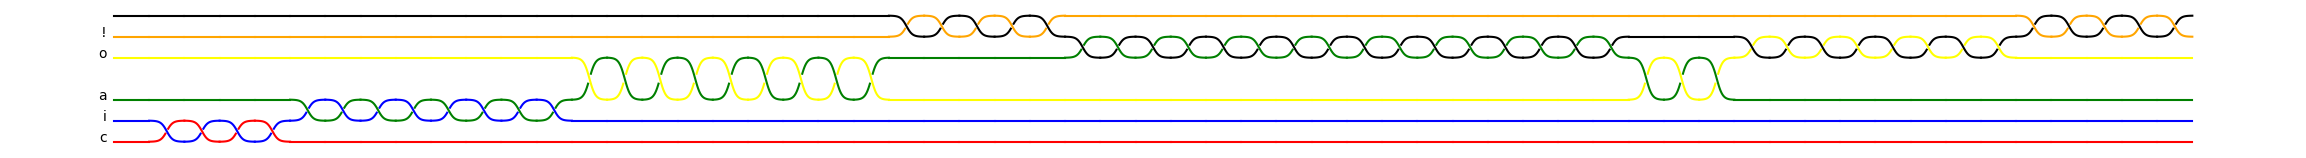
\includegraphics[width=0.45\linewidth]{images/ciaoOrdinato(1)(2).png}
\caption{Result for "Ciao"}
\end{figure}
\begin{figure}[!h]
\centering
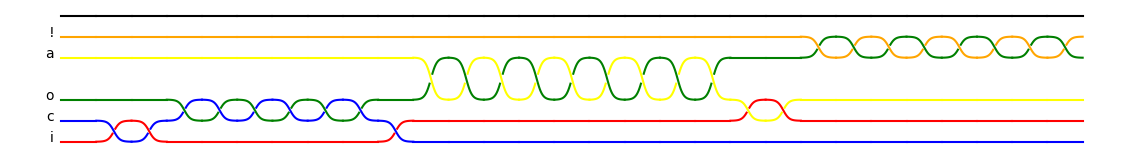
\includegraphics[width=0.45\linewidth]{images/ciaoDisord(1)(2).png}
\caption{Disordered message reordered by braiding}
\end{figure}

The images show a fundamental principle of topological quantum computing: information is stored in the braiding patterns of anyons, not in a fragile, local state.
\begin{itemize}
\item \textbf{Disordered Input}: The first image shows a set of tangled, braided lines. Each colored line represents an anyon, and their braiding encodes a disordered version of the word "ciao". This visually represents a chaotic or unstructured dataset. The unpredictable and erratic twists in the braids are similar to the noise ($\sigma_{noise}$) in a project trajectory, as seen in the scattered blue dots on the Bloch spheres.
\item \textbf{Ordered Output}: The second image shows the same anyons, but after a series of quantum operations -specifically, more braiding- they have been untangled and reordered. The orderly, clear connections at the end of the circuit represent a successful, structured output. This transformation from disorder to order is a visual metaphor for the goal of RQM: to take a project's chaotic, uncertain "pilot wave" and guide it toward a stable, predictable, and successful outcome.
\end{itemize}


This process of organizing a chaotic system through quantum transformations is at the heart of RQM. A quantum leader's role isn't to micro-manage every detail, but to perform "operations" that reduce the system's entropy and guide it toward a more ordered state.
\begin{itemize}
\item \textbf{Minimizing Uncertainty}: The braiding process visually represents the leader's work to minimize uncertainty. The complex, intentional braids serve to sort and organize the information, much like a leader applies principles and processes to reduce a project's bias and noise. The output, with its clear, parallel lines, shows a state of low entropy and high predictability-the ultimate goal of RQM.
\item \textbf{Fault Tolerance}: The "topological" nature of these circuits makes them incredibly resilient. Even if a small part of the braid is locally disturbed, the overall pattern remains intact. This directly relates to Topological Quantum Cybersecurity, where data is secured against local errors by its global properties. In RQM, this means that even if a small part of a project goes wrong, the overall trajectory remains on track because the system is robust and the leader has managed the overall "pilot wave," not just a single, fragile point.
\end{itemize}

\subsubsection*{Quantum Circuits for Data Encoding}
A different approach uses a standard quantum circuit with Ry and Rz gates to encode and protect data, such as the names and values from a data frame. This method uses quantum rotation gates to implement cryptographic principles and transmit information through a quantum channel.

\begin{figure}[!ht]
\centering
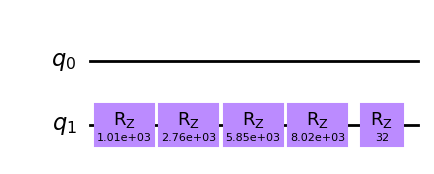
\includegraphics[width=0.45\linewidth]{images/quantCirc(1)(2).png}
\caption{Quantum Circuit with Ry/Rz Gates}
\end{figure}

\subsubsection*{Anyonic Circuit with Data}
The circuit shown in the image uses two qubits, labeled q0 and q1. The operations, represented by the purple boxes, are applied only to q1.
\begin{itemize}
\item \textbf{Qubits (q0, q1)}: These are the fundamental units of quantum information. They can exist in a superposition of states, allowing them to perform complex calculations in a way classical bits cannot.
\item \textbf{Rotation Gates (RZ)}: These gates, specifically Z-rotation gates, are a type of quantum operation that rotates the state of a qubit around the Z-axis of the Bloch sphere. The numbers inside the boxes (e.g., 1.01e+03, 2.76e+03) represent the angle of rotation. By applying a sequence of these rotations, you can precisely manipulate a qubit's state.
\end{itemize}


This circuit's design can be used to encode and protect information.
\begin{enumerate}
\item \textbf{Encoding Data}: The values of the Z-rotation gates can be used to encode data, such as the names and values from a data frame. For example, a name like "Alice" could be converted into a numerical sequence, which is then used as the rotation angles.
\item \textbf{Quantum Cryptography}: The manipulation of the qubit's state using these gates serves as the basis for a cryptographic key. The rotations act like a complex lock that can only be opened by applying the correct sequence of inverse rotations. Any attempt to intercept or measure the qubit's state would likely change it, alerting the user to an eavesdropper.
\item \textbf{Transmission}: After the data is encoded, the qubit can be transmitted through a quantum channel. The security of the information relies on the principles of quantum mechanics, where an observation (or eavesdropping attempt) on the qubit's state will inevitably disturb it.
\end{enumerate}


This standard quantum circuit approach, while different from the topological method, still aligns with RQM's core principles. It provides a more robust way to manage information in a chaotic environment. Unlike classical security systems that rely on linear, predictable processes, this method leverages the complex, probabilistic nature of quantum mechanics. It is about proactive security-ensuring the "pilot wave" of the data remains secure from the outset, rather than just reacting to a breach after it occurs.

\begin{figure}[!h]
\centering
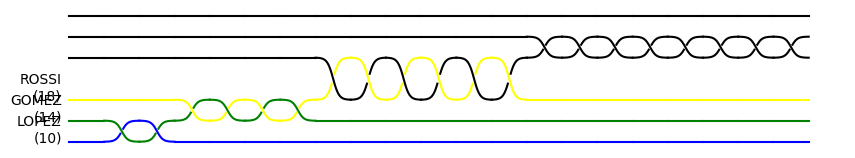
\includegraphics[width=0.45\linewidth]{images/anionCirc(1).png}
\caption{Anyon Circuit for Data Transmission}
\end{figure}
\newpage
\section{Risk Management within Relativistic Quantum Management Framework}
\label{sec6}
The risk management is an essential part of the Insurance Sector \cite{riskDef}. Indeed, it is crucial to have correct computation for the goal of making right predictions and right actuarial outputs.

Given that the real innovation does not lie in changing the mathematical fundamentals but in applying cutting-edge computational approaches to execute them with unprecedented speed, scale, and accuracy, I will describe an application of Relativistic Quantum Management in the computation of some features of the Risk Management.

In the following, I will show you some applications with quantum circuits and quantum versions of some algorithms.
Quantum computing provides the essential tools to make this new approach to risk management practical. While the philosophical framework of quantum management is about a mindset shift, quantum computers offer the computational power to execute the complex calculations required.

Quantum computers can significantly enhance Monte Carlo simulations, which are a cornerstone of modern risk modeling. By leveraging quantum principles like superposition and entanglement, they can explore a vast number of scenarios simultaneously, possibly providing faster estimations of risk metrics like Value-at-Risk (VaR) and Conditional Value-at-Risk (CVaR). In finance, quantum algorithms can solve complex optimization problems to construct a portfolio that minimizes risk for a given level of return. This can be done in real time, allowing institutions to react instantly to market fluctuations. For scenarios like stress testing a global supply chain or a financial system, quantum computers can model the interconnectedness and potential cascading failures in a way that is computationally intractable for classical computers.

\subsection{Best Estimate Unit Linked}
The Best Estimate (BE) unit-linked method is a specific approach used in actuarial science and finance to calculate the value of insurance liabilities, particularly for unit-linked life insurance policies. This method stands out because it separates the calculation of the policy's value into two distinct parts: the unit fund and the non-unit liabilities
The term "best estimate" emphasizes that the assumptions used are unbiased. Unlike older, more conservative methods that built in significant safety margins, this approach aims to be as accurate as possible based on a realistic assessment of future events. This provides a more transparent and consistent measure of a company's financial health, particularly under modern regulatory frameworks like Solvency II.
The code following sets up a conceptual classical neural network using Python, TensorFlow, and Keras.
\begin{enumerate}
    \item It generates synthetic financial data (BEUL) and preprocesses it for model training using standard scaling
    \item The model's architecture combines classical Dense layers with a placeholder for a quantum circuit to demonstrate a hybrid approach
    \item It trains the model using a standard adam optimizer and mse loss, treating the quantum part as a differentiable layer
    \item Finally, the code evaluates the model's performance and uses it to make a prediction on new, unseen data
\end{enumerate}
Predicted BEUL for the new scenario: $10091.54$
The following code sets up a conceptual hybrid quantum-classical neural network using Python, TensorFlow, and Keras.
\subsection{Best Estimate Unit Linked Quantum Version}
\begin{enumerate}
    \item It includes functions (state to bloch, bloch to state) that use the Qutip library to demonstrate the mathematical representation of quantum states on the Bloch sphere
    \item A placeholder function (create quantum circuit) simulates generating random mixed quantum states for a conceptual quantum layer
    \item The model architecture consists of classical Dense layers, with a commented-out line for a quantum layer, demonstrating a hybrid structure
    \item The model is trained and evaluated classically, serving as a conceptual proof of a hybrid workflow rather than a fully functional quantum neural network
\end{enumerate}
Predicted BEUL from the hybrid model: $10076.16$\\\\
The model starts with synthetic financial data (BEUL) and processes it to make it suitable for training. A neural network is built using standard layers, with a designated space for a quantum component to be added later, then the model is trained to minimize prediction errors and then used to forecast the BEUL value for a new, unknown scenario. The prediction of $10,091.54$ is a single, deterministic number.


This approach is good, but it gives a single answer. RQM, however, knows that a single prediction isn't enough in an uncertain world.


The quantum version takes the classical model a step further by introducing concepts from quantum mechanics. This is where the true RQM mindset comes in, viewing the system not just as a set of data points, but as a dynamic and probabilistic whole.
\begin{enumerate}
\item \textbf{Modeling Quantum States}: The code uses the Qutip library to represent a policy's state on a Bloch sphere. This is a core RQM concept, where a single point on the sphere represents an ideal, "pure" state, while a distribution of points represents the uncertainty and all possible outcomes.
\item \textbf{A Probabilistic View}: The model includes a conceptual "quantum layer" that can generate random mixed quantum states. In RQM, this represents the "pilot wave"---a field of all possible scenarios and behaviors of policyholders. The model acknowledges that a customer's behavior isn't fixed; it is a superposition of possibilities.
\item \textbf{Training and Prediction}: The model is trained to learn from these complex, probabilistic states. The final prediction of $10,076.16$ is subtly different from the classical model's. This difference isn't an error; it could be a reflection of the model's understanding of risk, taking into account the nuanced, interconnected nature of financial systems.
\end{enumerate}
In essence, the classical model provides a single number, while the quantum model provides a glimpse into the distribution of probabilities that form that number. This allows a quantum manager to not just know a value, but to understand the range of potential outcomes and proactively manage the risks within that uncertainty.
\subsection{Modeling Policyholder Behavior within Relativistic Quantum Managment}
This model uses a powerful tool called an Agent-Based Model to simulate customer behavior.
\begin{enumerate}
\item \textbf{Individual Policyholders as Qubits}: In this model, each policyholder is treated as a qubit from quantum computing. A qubit can be in a superposition of states---in this case, a customer is in a mix of "will stay" and "will cancel" states. This is visualized on a Bloch sphere, where a point represents a specific mix of these two possibilities.
\item \textbf{Lapse Decision}: The decision to cancel a policy isn't random. It is influenced by a combination of factors:
\begin{itemize}
\item The qubit's state: A key factor is the z-component of the qub state. Think of this as a measure of the customer's inherent stability or instability. A higher value on the z-axis means the customer is less likely to cancel.
\item \textbf{External factors}: The model also considers external influences like the customer's premium and their personal aversion to risk.
\end{itemize}
\item \textbf{Simulation}: The simulation runs through different time steps to see how a portfolio of customers evolves. It calculates how many customers will lapse based on these factors, as well as the premiums offered by competitors.
\item \textbf{Visualizing the Results}: The outcome is a graph that shows the number of active policies decreasing over time. This isn't just a simple line; it is a visual representation of the decay of a system, much like how a quantum particle decays.
\end{enumerate}


This approach is fundamentally different from a classical one. A classical model might give you a single, average lapse rate. A RQM-inspired model, however, shows you the entire distribution of possible outcomes.

By modeling policyholders as dynamic quantum states, an insurer can:
\begin{itemize}
\item \textbf{Predict with Uncertainty}: Instead of a single number, the model provides a more realistic view of risk, acknowledging that a customer's decision is not fixed but probabilistic.
\item \textbf{Proactively Manage}: A quantum manager can use this model to identify which policyholders are in a more unstable state (i.e., their qubit's z-component is low) and intervene with targeted offers or communication to prevent them from lapsing.
\end{itemize}
This method allows insurers to move from simply reacting to policy cancellations to proactively managing a portfolio by understanding the underlying quantum-like behaviors of their customers.
\subsubsection{The Mathematics of Policyholder Behavior with Agent Based Model}
\begin{enumerate}
    \item Each policyholder agent is assigned a quantum-inspired state, represented as a qubit on the Bloch sphere using the qutip library
    \item The decision to lapse is influenced by a factor derived from the z-component of the qubit state, combined with their premium and risk aversion
    \item The run simulation function iterates through time steps, calculating lapses based on competitor premiums and recording the number of active policies
    \item The results are visualized in a plot showing the decay of active policies over time, modeling a quantum-inspired management process
\end{enumerate}

\begin{figure}[!ht]
    \centering
    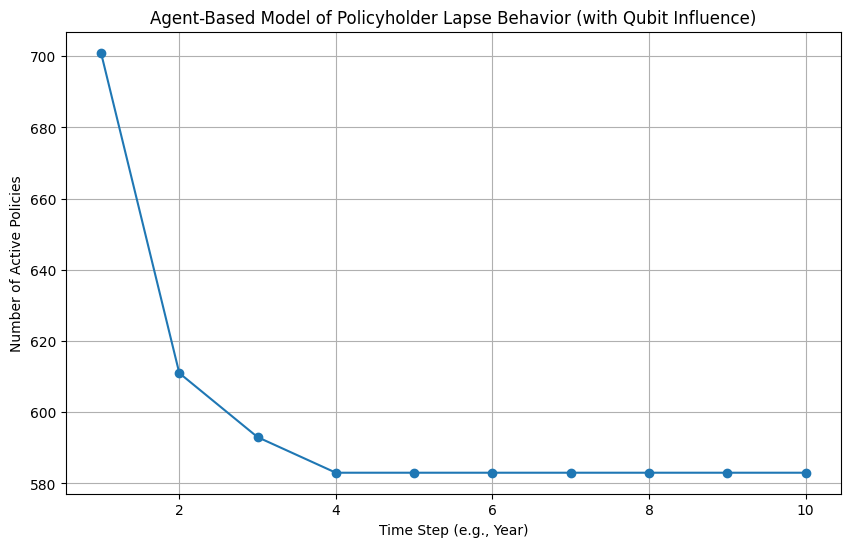
\includegraphics[width=0.5\linewidth]{images/policyholderBehaviourQuantum(1).png}
    \caption{Policyholder Behavior}
\end{figure}
\subsection{Quantum Chain Ladder}
\begin{enumerate}
    \item Iterative Training: The code runs for a specified number of epochs (100 in this case), with each epoch representing a full pass through the training data
    \item Data Encoding: For each data point, angular encoding maps the classical features (like scaled claims data) and a raw cumulative loss value into quantum-friendly input angles
    \item Quantum Processing: The pqc (Parameterized Quantum Circuit) processes these angles using learnable parameters (initial params), which are optimized during training
    \item Prediction and Loss Calculation: The circuit's output, an expectation value, is then converted into a predicted ultimate loss. This prediction is compared against the actual target loss (y train torch) to compute the loss for that data point
    \item Parameter Update: The optimizer uses the total loss from the epoch to calculate gradients via backpropagation (total loss.backward()) and updates the PQC's parameters (optimizer.step()), aiming to minimize the loss in the next epoch
\end{enumerate}
\begin{figure}[!ht]
    \centering
    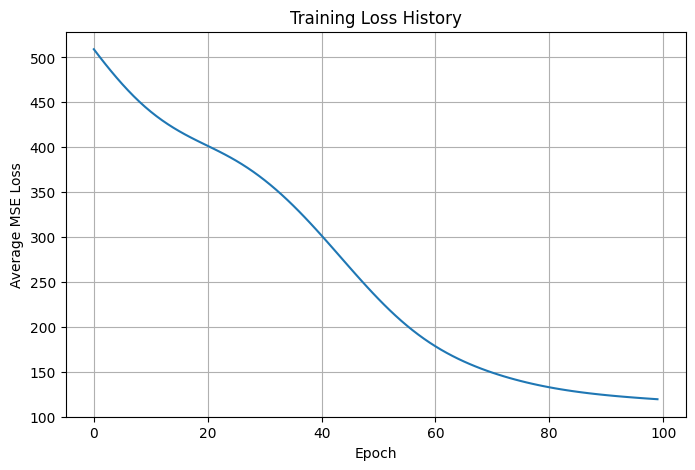
\includegraphics[width=0.4\linewidth]{images/qcl(2).png}
    \caption{MSE}
\end{figure}
\subsubsection*{How the Training Process Works}
The process is an iterative loop designed to teach the model how to make accurate predictions.
\begin{enumerate}
\item \textbf{Data Encoding}: First, the model takes classical data and converts it into a format a quantum computer can understand. This is called angular encoding, where each piece of data is mapped to a specific angle, which then becomes an input for the quantum circuit.
\item \textbf{Quantum Processing}: The encoded data is then fed into the PQC, a quantum circuit with adjustable parameters. The PQC processes the data using quantum principles like superposition and entanglement to perform complex calculations.
\item \textbf{Prediction and Loss Calculation}: The quantum circuit's output, an "expectation value," is then converted back into a classical prediction. This prediction is compared to the actual target value to calculate the loss, which measures how far off the prediction was. A lower loss means a more accurate prediction.
\item \textbf{Parameter Update}: The optimizer uses the calculated loss to adjust the PQC's parameters. This is a process called backpropagation, where the model learns from its mistakes and updates its internal settings to make a better prediction in the next training cycle. This iterative process repeats for a set number of epochs (100 in this case).
\end{enumerate}

\subsubsection*{Analyzing the Training Loss History}
The graph titled "Training Loss History" visually represents this learning process.
\begin{itemize}
\item \textbf{X-axis (Epoch)}: This shows the number of training cycles the model has completed. Each epoch represents one full pass through the entire training dataset.
\item \textbf{Y-axis (Average MSE Loss)}: This measures the average prediction error, or "loss," for each epoch.
\end{itemize}
As the number of epochs increases, the curve on the graph steadily decreases. This shows that the model is continuously learning and improving its predictions with each training cycle. By the end of the 100 epochs, the loss is significantly lower than when it started, indicating that the model has become much more accurate at predicting the target values. This successful training process confirms that the hybrid quantum-classical model can effectively handle and learn from complex, real-world data, making it a valuable tool for risk management within the RQM framework.
\subsection{Quantum Ising Model for Swiss Financial Credit Risk}
Swiss financial institutions use mathematical models to simulate and quantify credit risk, moving beyond simple static analysis. The core of these models involves a blend of statistical methods and stochastic processes to forecast potential losses under various scenarios.


Instead of just looking at individual loans, Swiss banks model their entire \textbf{credit portfolio} to understand the aggregate risk. The goal is to estimate the probability distribution of future losses over a given time horizon (e.g., one year). The total loss ($L$) of a credit portfolio is the sum of losses from each loan ($L_i$):

$$ L = \sum_{i=1}^{N} L_i $$

The loss from an individual loan ($L_i$) is a random variable determined by three key factors:

$$ L_i = \text{EAD}_i \times \text{LGD}_i \times \text{PD}_i $$

\begin{itemize}
    \item \textbf{PD (Probability of Default)}: The probability that a borrower will fail to meet their obligation.
    \item \textbf{LGD (Loss Given Default)}: The percentage of the exposure that the bank loses if a default occurs.
    \item \textbf{EAD (Exposure at Default)}: The amount of money the bank is owed at the time of default.
\end{itemize}

A Monte Carlo simulation is used to model the uncertainty in these variables. The process involves several steps:

\begin{enumerate}
    \item \textbf{Model the Economy}: The simulation begins by generating a large number of random economic scenarios (e.g., thousands or millions) that reflect factors like GDP growth and unemployment. The correlation between these factors is a crucial input.
    \item \textbf{Link Economic Factors to PD}: A statistical model links the overall economic conditions to the individual probability of default for each borrower, capturing the fact that defaults are often correlated.
    \item \textbf{Generate Default Events}: For each economic scenario, a random number is generated for each loan. If this number is below the calculated PD, the loan defaults.
    \item \textbf{Calculate Losses}: If a default occurs, the model then simulates the LGD and EAD to calculate the total loss for that specific scenario.
    \item \textbf{Repeat and Aggregate}: This process is repeated thousands of times. The results are aggregated to create a \textbf{distribution of potential losses} for the entire portfolio.
\end{enumerate}

The output of these simulations is the \textbf{Loss Distribution Curve}. This curve is a powerful tool for Swiss financial managers:

\begin{itemize}
    \item \textbf{Capital Requirements}: Regulators use this loss distribution to determine the amount of capital a bank must hold to cover potential unexpected losses, often set at a very high confidence level (e.g., the 99.9\% Value-at-Risk, or VaR).
    \item \textbf{Risk Management}: The simulation identifies which sectors or types of loans contribute most to the total risk, guiding decisions on portfolio diversification.
    \item \textbf{Stress Testing}: By simulating extreme, adverse economic scenarios, banks can test their resilience and prepare for crises.
\end{itemize}


My analysis shows that the Quantum Ising Model provides a potentially accurate way to model the interconnected risks in a financial portfolio. This is a core tenet of Relativistic Quantum Management: using quantum-inspired methods to better understand and proactively manage the complex, chaotic systems of the real world.
\begin{enumerate}
    \item It uses a predefined list of obligors, each with a credit rating, exposure, default rate, and standard deviation
    \item The quantum Ising model simulation function uses a classical approximation of a quantum system to model correlated defaults, where a spin-flip is analogous to an obligor's default
    \item The simulate credit portfolio function uses a more traditional Monte Carlo method, where default rates are adjusted by economic factors
    \item Both simulations generate a distribution of portfolio losses, and the code then calculates and compares key risk metrics like Mean Loss, Standard Deviation, and Value-at-Risk (VaR)
\end{enumerate}
\begin{itemize}
\item \textbf{Monte Carlo Simulation}: This is a classic risk management tool that uses random sampling to model the probability of different outcomes. The simulation adjusts a company's default rate based on various economic factors. While powerful, this approach can be computationally intensive and may not fully capture the complex, interconnected nature of a financial system.
\item \textbf{Quantum Ising Model}: This model uses a concept from physics to model the risk of correlated defaults. Each company in a portfolio is analogous to a "spin" that can be in one of two states: "up" (no default) or "down" (default). The interactions between these spins represent the correlations between companies, allowing the model to handle these complex relationships more efficiently than a classical computer.
\end{itemize}

\subsubsection*{Analyzing the Graphs}
The output \ref{fig:mcs} directly compares the results of the two models.
\begin{itemize}
\item \textbf{Loss Distribution Comparison}: The top-left graph shows that the Quantum Ising Model's distribution (red bars) is narrower and taller than the Monte Carlo model's (blue bars). This suggests the quantum model predicts a lower overall loss but a higher probability for certain loss events.
\item \textbf{Cumulative Distribution Functions (CDFs)}: The top-right graph shows that the Quantum Ising model's CDF (red line) is steeper than the Monte Carlo model's (blue line). This indicates a more concentrated probability around the mean.
\item \textbf{Corresponding Losses Comparison}: The bottom-left graph shows that the two models are generally in agreement, but there are notable differences, especially for larger loss amounts. This highlights that the Quantum Ising Model provides a unique perspective on the distribution of risk.
\item \textbf{Distribution of Differences}: The box plot on the bottom-right confirms the overall agreement between the models, but the outliers (circles) show significant disagreements in specific, high-risk scenarios.
\end{itemize}
\begin{figure}[!ht]
    \centering
    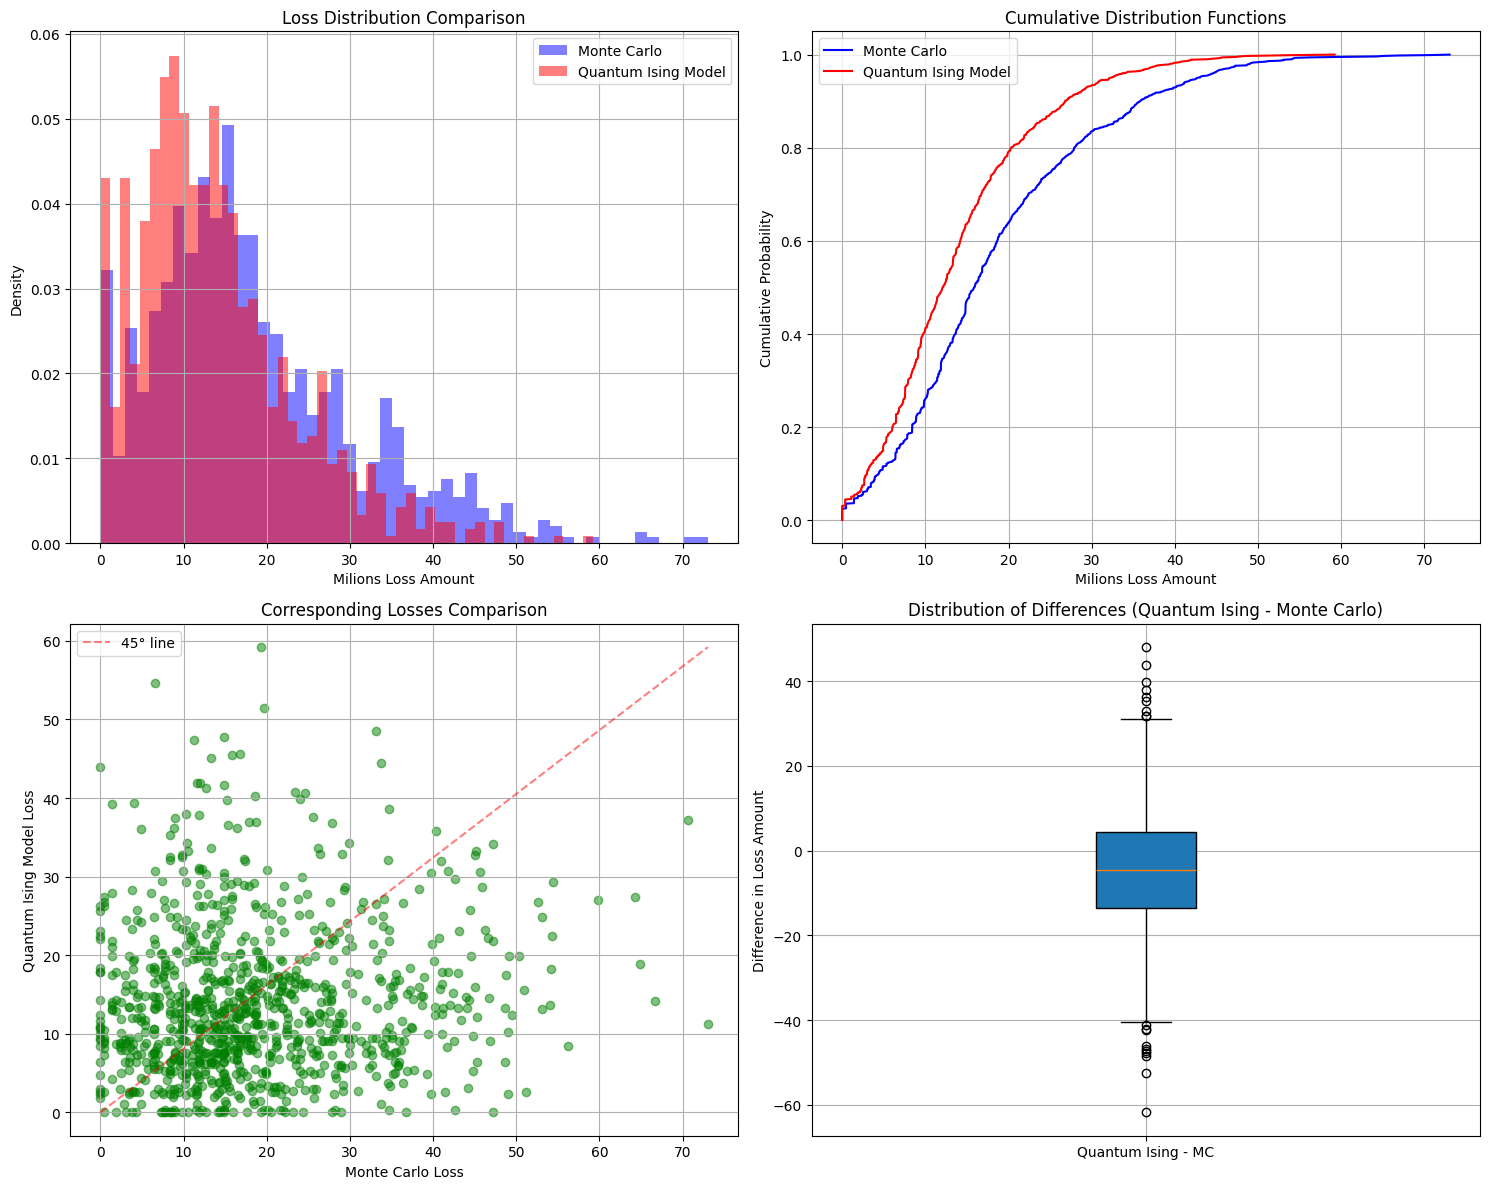
\includegraphics[width=0.5\linewidth]{images/rmcrqm(2).png}
    \caption{Simulation Swiss Credit Risk with Quantum Ising Model}
    \label{fig:mcs}
\end{figure}


\newpage
\section{Customer Centricity and Statistical Customer Analysis within Relativistic Quantum Management Framework}
\label{sec7}
Customer centricity is a business strategy that puts the customer at the center of a company's decisions and operations.\\It's not just about offering good customer service, instead, it's a holistic philosophy where the business's success is directly tied to the customer's satisfaction and long-term loyalty. In today's competitive market, a strong customer-centric culture could be a unique and durable advantage. It appears that companies that master this strategy often see higher customer retention, increased revenue, and more effective word-of-mouth marketing, making them more resilient and profitable in the long run.

Customer centricity, indeed, represents a paradigm shift in the insurance industry, moving from a product-focused model to an approach that places the customer at the heart of all decisions and operations. This transformation is largely driven by insurtechs, which apply advanced technologies to create smoother, more personalized, and transparent experiences. This document explores the principles of customer centricity and discusses how insurtechs are applying them to innovate in the market.


Historically, insurers operated on a product-centric model. The focus was on creating standardized products and selling them through traditional channels like agents and brokers. The customer journey was often complex and bureaucratic, characterized by long forms, time-consuming claims processes, and a lack of transparent communication. This approach resulted in low customer satisfaction and a lack of loyalty.


Customer centricity, in contrast, is built on four fundamental pillars:
\begin{enumerate}
\item \textbf{Personalization}: Offering products and services tailored to the specific needs and behaviors of each customer.
\item \textbf{Transparency}: Ensuring clarity in communication, from policy subscription to claims resolution.
\item \textbf{Efficiency}: Simplifying and accelerating all processes, using technology to eliminate friction.
\end{enumerate}


Insurtechs are technology startups that aim to enhance the insurance industry. Their digital architecture and lack of legacy systems allow them to apply customer centricity natively and effectively.


Several insurtechs and innovative companies exemplify the application of customer centricity:
\begin{itemize}
\item \textbf{Lemonade}: Known for its business model driven by artificial intelligence (AI) and its transparent approach. AI streamlines the underwriting and claims process, allowing for the resolution of simple claims in seconds. Their platform is intuitive, and the focus on user experience is evident.
\item \textbf{Zego}: An insurtech specializing in insurance for the gig economy and commercial drivers. Its flexible and dynamic pay-as-you-go pricing model is a perfect example of personalization, adapting the insurance cost to the actual behavior and use of the vehicle, which is highly valued by this customer segment.
\item \textbf{Kin Insurance}: Focused on homeowners' insurance in catastrophe-prone areas. Kin uses big data and AI to accurately assess the individual risk of each property. This allows them to offer personalized policies and competitive prices, ensuring that customers in high-risk zones have access to adequate coverage. Their platform simplifies the customer journey, from quote to claim.
\end{itemize}


The technologies that enable customer centricity include:
\begin{itemize}
\item \textbf{Artificial Intelligence (AI) and Machine Learning}: Used to automate processes, personalize prices and offers, and analyze large volumes of customer data for behavioral insights.
\item \textbf{The Internet of Things (IoT)}: Devices like telematics in cars or sensors in homes allow for real-time data collection, enabling usage-based insurance models and proactive prevention strategies.
\item \textbf{Advanced Data and Analytics}: The ability to collect, integrate, and analyze data from various sources allows for a 360-degree view of the customer, which is fundamental for personalization and anticipating their needs.
\end{itemize}

In order to adopt a centric optic around the customer it is necessary to be aware of the psychology and of the insurance hierarchy.
Indeed, it would be interesting to consider the realization of ad hoc policies, that help people individually, taking into account their necessities and preferences.

Modelling customers preferences is a good strategy that companies adopt to produce statistical analysis which is implemented to review product and/or product new ones, also based on customer preferences.

An important marketing strategy is the segmentation that could reach its extrema in "One-to-one approach". A case study is "Nikye" that decorates shoes based on customers preferences.

To focus on a customer-centric approach, especially in the insurance sector, it is essential to understand customer psychology and tailor services to individual needs rather than treating customers as a single group. This leads to a one-to-one approach, where the goal is to create personalized policies and products.

This one-to-one strategy is built on four key pillars:
\begin{itemize}
\item \textbf{Customer Identification}: Gathering detailed data on each person's behavior, preferences, and interactions, going beyond basic demographics to build a complete profile.
\item \textbf{Customer Differentiation}: Using this detailed data to group customers based on their value and needs, allowing a company to offer exclusive benefits to its most loyal customers.
\item \textbf{Personalized Interaction}: Customizing communication, such as sending emails with product recommendations based on a customer's browsing history, to make them feel valued.
\item \textbf{Customization}: Tailoring the product or service itself to a customer’s specific requirements.
\end{itemize}

\subsection{The Relativistic Quantum Management Approach}
Relativistic Quantum Management (RQM) provides a framework for the insurance sector to adopt this one-to-one approach. It uses concepts from quantum mechanics to model customer satisfaction and product development.

Indeed, by reconsidering the mathematics of the Pilot Wave and the goal of one-to-one approach in marketing:
\begin{equation}
    \psi_{curstomerSatisfaction} = e^{iS_{customerFeedback}/product}
\end{equation}
where $S_{customerFeedback}$ is the phase of the pilot global wave.
I then define a velocity of it:
\begin{equation}
   v_{customerSatisfaction} =  \frac{dq}{dt} =  \frac{NumberOfProducts}{Time} \nabla{S_{CustomerFeedback}(A,Q)}
\end{equation}
where the gradient depends on the adequacy A and quality Q of the product. q(t) is the trajectory.\\
The diffusion of the wave is as follows:
\begin{equation}
    J = w(A, Q)_i \frac{d \rho_{sprint_{CustomerSatisfaction}}}{dt}
\end{equation}
The diffusion is related to a weight of adequacy (A) and of quality(Q), and to the mixture density state associated to a sprint backlog. It is inspired by Fick's law.\\
Indeed, the entropy of the whole ensemble, in a relative time, would be given by
\begin{equation}
    dS_{CustomerSatisfaction} = \sum_i (d\rho_i \cdot p_i \cdot w(A, Q)_i) t_{relative}
\end{equation}
where p is the probability related to such mixture state of a sprint and w is the weight of priority and quality associated to the sprint of the specific task, within absolute time.\\
\begin{equation}
    \frac{\partial S}{\partial \rho_i} = w_i p_i t_{relative}
\end{equation}
where the evolution of the mixture state is given by Von-Neumann, inspired by Liouville:
\begin{equation}
    d\rho_i = \frac{\partial{\rho_i}}{\partial t} + \{H, \rho_i\} =0
\end{equation}
The clue is to get $S = 0$.
The total energies would respect the statistics as follows:
\begin{equation}
    A = U - TS (V,T const)
\end{equation}
\begin{equation}
    G = H - TS (P, T const)
\end{equation}
\\\\
Now, what it would be possible, is to include the evolution in a relative time, for every possible scenario, therefore:
As $N \to \infty$, the multiple integral becomes something unknown to the mathematics of the time, and Feynman calls it a path integral in the configuration space, introducing the following notation:
\begin{align}
\phi\epsilon\rho\omega(q_b, t_b; q_a, t_a) = \int_{q(t_a)=q_a; q(t_b)=q_b} \mathcal{D}^f scneario(\cdot) e^{\frac{1}{proactivity} \int_{t_a}^{t_b} dt \mathcal{L}(scenario(t), \dot{scenario}(t))}\\ = \int_{q(t_a)=q_a; q(t_b)=q_b} \mathcal{D}^f scenario(\cdot) e^{\frac{i}{proactivity} S_{CustomerFeedback}} 
\end{align}
Here the quantum term is given by proactivity. 

Proactivity is made possible by leveraging data and technology to create highly personalized, predictive interactions. The goal is to build stronger customer relationships by demonstrating that the company understands and cares about the individual's specific situation. 

Here's how the key variables in the model relate to real-world business concepts:
\begin{itemize}
\item \textbf{Customer Satisfaction Pilot Wave ($\psi_{customerSatisfaction}$)}: This wave is a mathematical representation of customer satisfaction, with its phase ($S_{customerFeedback}$) being influenced by the feedback received on a product.
\item \textbf{Trajectory of the Wave (q(t))}: This is the path the customer satisfaction takes over time. The velocity of the wave ($v_{customerSatisfaction}$), which represents how fast customer satisfaction changes, is determined by the number of products and a gradient ($\nabla$) of customer feedback. This gradient depends on two critical factors:
\begin{itemize}
\item \textbf{Adequacy (A)}: How well a product meets a customer's needs.
\item \textbf{Quality (Q)}: The overall quality of the product.
\end{itemize}
\item \textbf{Diffusion of the Wave (J)}: This describes how changes in customer satisfaction spread throughout the system, like how a successful product launch might influence overall brand perception. This diffusion is influenced by a weight (w) that reflects the importance of a product's adequacy and quality. It also depends on the mixture density state ($\rho$), which represents the blend of different tasks in a project's "sprint backlog."
\item \textbf{Entropy (S)}: In this model, entropy measures the level of disorder or imbalance in customer satisfaction. The ultimate goal is to reach a state of S=0, which signifies perfect balance and customer satisfaction. The evolution of this system is governed by a principle similar to the Von-Neumann equation, where changes are driven by a force that pushes the system towards equilibrium.
\item \textbf{Proactivity}: In RQM, proactivity is a core principle. It is the ability of an organization to anticipate future needs and act before problems arise. It is so fundamental that it is the "quantum" term in a Path Integral, which is a powerful mathematical tool used to model all possible future scenarios.
\end{itemize}


Proactivity is the ability of an organization to anticipate customer needs, market changes, and potential risks, and to act on them before they become problems. This goes beyond simply responding quickly (adaptiveness) and involves forward-looking, preemptive action.

 
 Proactivity can be measured by how well an organization foresees future trends and customer needs.
 \begin{itemize}
 	\item \textbf{Early Warning Indicators (EWI) Score}: A quantitative measure of how often the company successfully identifies emerging trends or potential risks before they become widely known. This can be tracked by comparing the company's internal reports on emerging risks to their eventual market impact.
 	\item \textbf{Customer Needs Prediction Accuracy}: The percentage of new product features or ad hoc policies that were developed based on predicted customer needs and were subsequently adopted by the customers. A higher percentage indicates more effective anticipation and proactivity.
 	\item \textbf{Predictive Product Development}: The average time between a company's internal identification of a potential future need and the launch of a product designed to meet that need. Shorter times indicate greater proactivity.
 \end{itemize}
 
 
 Proactivity is not just about prediction; it is about acting on that prediction.
 \begin{itemize}
 	\item \textbf{Proactive vs. Reactive Actions Ratio}: The number of initiatives launched in response to a predicted need (proactive) versus those launched in response to a current problem or competitor's move (reactive). A higher ratio demonstrates a more proactive culture.
 	\item \textbf{Budget Allocation to Foresight}: The percentage of a company's R\&D or innovation budget dedicated to speculative, future-oriented projects rather than incremental improvements or reactive fixes.
 	\item \textbf{Lead Time of Policies}: For ad hoc insurance policies, the time between when a policy is designed and when it is needed. A negative lead time (the policy is needed before it is designed) would indicate a reactive system, while a positive lead time indicates proactivity.
 \end{itemize}

 
 A truly proactive organization has a robust feedback mechanism that continuously refines its predictive models.
 \begin{itemize}
 	\item \textbf{Foresight Learning Cycle}: A metric that tracks how a company incorporates the outcomes of its proactive measures (both successes and failures) into its future predictive models. This ensures that the organization gets "smarter" over time.
 	\item \textbf{Entropy Reduction Index}: Inspired by the goal of $S=0$, this could be a composite index that measures the reduction of "disorder" or uncertainty in the system. It could be calculated by assessing the variance in customer satisfaction and product performance over time, with a lower variance indicating a more proactive and stable system.
 \end{itemize}
 
Proactivity is made possible by leveraging data and technology to create highly personalized, predictive interactions. The goal is to build stronger customer relationships by demonstrating that the company understands and cares about the individual's specific situation. This is possible aboveall by appyling the psychology.


Let's start by considering the psychological behavior of a policyholder. Indeed, there are some factors which are crucial in depicting the idenitity kit.

 Some are Risk Aversion: Individuals differ in their willingness to take risks. Those who are highly risk-averse are more likely to purchase insurance and file claims for even minor incidents; Loss Aversion: People are psychologically more motivated to avoid a loss than to achieve an equivalent gain. This can make them reluctant to let a policy lapse if they feel they are losing a benefit, even if the financial logic suggests otherwise; Cognitive Biases: Mental shortcuts, or heuristics, can lead to irrational decisions. For example, the availability heuristic might cause a person to overstate the risk of a flood after seeing a news report, making them more likely to purchase flood insurance; Social Proof: Policyholders are often influenced by the actions of their peers. If an insurance company can show that "everyone else is buying this policy," it can psychologically validate the decision for a potential customer; Trust: A policyholder's trust in their insurance company is a crucial factor in both retention and claim filing. A lack of trust can lead to higher lapse rates.\\
Individuals that decide to hold a policy, they do it in a situation charcterized by uncertainty, by a mechanism called "if-so": If it happens an accident, so I can use the policy.\\
Kahneman's Prospect Theory explains how people make decisions under uncertainty. A core tenet is loss aversion: the psychological pain of a loss is roughly twice as powerful as the pleasure of an equivalent gain. Instead of highlighting what a customer can gain, marketers often focus on what they stand to lose by not acting. Example: An insurance ad might emphasize the financial devastation of a house fire (a loss) rather than the peace of mind gained from a policy. Limited-time offers also trigger loss aversion by creating the fear of missing out on a deal; The anchoring effect is a cognitive bias where an individual relies too heavily on the first piece of information offered (the "anchor") when making a decision; Marketing Application: Marketers use a high initial price (the anchor) to make a subsequent, lower price seem more attractive. Example: A product originally listed at 500 and then "on sale" for 250 appears to be a great value, even if its true worth is closer to the sale price.\\\\
The essential tool in marketing is the \textit{communication} or how information is presented. 

In this process, System 1 thinking reacts strongly to how a message is framed, regardless of its logical content, in this environment, marketing can work very well with some tricks: for example, marketers can frame a product positively or negatively to sway a consumer.
Example: A beef product described as "75\% lean" is seen as healthier and more appealing than one described as "25\% fat," even though they are mathematically the same. This also applies to risk; a medical treatment with a "90\% survival rate" is more attractive than one with a "10\% mortality rate."; Mental accounting is the tendency for people to categorize and budget money in separate mental accounts, often irrationally; Marketing Application: Marketers can encourage spending by framing it in a way that aligns with a consumer's mental accounts. Example: Offering a rebate or gift card (which feels like "found money") rather than a direct discount can encourage additional purchases. People are more likely to spend money from a rebate than from their regular income.\\\\
The availability heuristic is a cognitive bias where individuals overestimate the probability of events that are easily recalled from memory. In the insurance industry, this psychological shortcut is a powerful driver of consumer behavior. A low-probability event, such as a natural catastrophe, receives extensive media coverage, making it highly salient in the public consciousness. This heightened visibility leads to an inflated perception of risk that is disproportionate to the actual long-term probabilities.\\\\
This phenomenon gives rise to the waterfall of availability, a self-reinforcing loop where a vivid event, amplified by media, triggers public fear and a cascade of institutional or governmental responses. These responses, in turn, validate and reinforce the public's heightened sense of risk, driving a surge in demand for related insurance policies. For marketers, this loop represents a powerful tool to influence consumer behavior by leveraging an event-driven emotional state.\\\\
The affect heuristic posits that individuals rely on their immediate feelings and emotional responses to make judgments and decisions. People often fear rare, insidious threats like botulism more than statistically deadlier, more common events like lightning strikes. This demonstrates that the emotional intensity associated with an outcome, rather than its objective probability, is a primary driver of perceived risk.


In this context, marketing campaigns that appeal to emotional triggers such as fear, hope, or a sense of security can bypass the slow, deliberate processing of System 2 thinking and directly influence the fast, intuitive responses of System 1. Research in neuroeconomics, particularly studies on individuals with prefrontal cortex damage, shows that the inability to process emotions significantly impairs decision-making, reinforcing the inseparable link between feeling and choice.\\\\
The concept of risk itself is not a tangible entity but rather a mental construct. According to psychologist Paul Slovic, a "real risk" does not exist independently of our minds. The perception of risk is inherently subjective, shaped by our beliefs, values, and emotional state. This insight is foundational for marketing, as it suggests that the effectiveness of an insurance campaign depends less on a precise quantification of risk and more on its ability to shape the emotional and psychological perception of that risk.


Furthermore, the illusion of validity contributes to this subjectivity. This bias refers to a person's tendency to form confident conclusions from limited evidence. The credibility of a source, rather than the quality of the data, often dictates a person's belief. This is why testimonials from "experts" or "trusted sources" are effective; they appeal to our reliance on authority to validate our beliefs, circumventing the need for logical scrutiny by System 2.


Several other behavioral biases have direct implications for insurance and financial marketing:
\begin{itemize}
\item \textbf{The Fear of Regret}: This is the psychological discomfort associated with anticipating a bad outcome from a non-standard decision. It can lead individuals to conform to social norms, such as purchasing a standard insurance policy, even if a more optimal, less conventional choice exists.
\item \textbf{The Disposition Effect}: While typically applied to investing, this bias highlights the human tendency to hold onto losing positions too long while selling winners too early. In the context of insurance, it reflects a similar emotional aversion to realizing a loss, which can influence decisions related to policy cancellations or claims.
\end{itemize}

In conclusion, human beings are not purely rational economic agents. By leveraging the principles of behavioral economics and cognitive psychology, marketers can influence consumer perception and behavior more effectively than with a purely factual presentation of risk. This approach focuses on appealing to System 1 thinking through emotional triggers, exploiting cognitive shortcuts like the availability heuristic, and using a strategic framing that minimizes the fear of regret. This model of marketing shifts the focus from an objective risk assessment to the subjective and emotional experience of the customer, fundamentally reshaping how insurance products are communicated and sold \cite{kahneman2011thinking}.

\subsubsection{Policyholder Behavior through the Prospect Theory lens}
The observation that individuals consistently purchase both insurance policies and lottery tickets poses a significant challenge to traditional economic theory. Both actions involve a negative expected monetary value; one pays a premium to avoid a potential large loss (insurance), while the other pays a small amount for a chance at a large gain (lottery) \cite{kahneman1979prospect}.

Conventional utility theory attempts to explain this behavior through the shape of the utility function for money. A commonly held assumption is that utility is a \textbf{concave function of wealth}, implying that the marginal utility of wealth decreases as one's wealth increases. This explains \textbf{risk aversion} and the purchase of insurance, as individuals are willing to pay a premium to avoid a large, uncertain loss.

However, this same assumption fails to account for \textbf{risk-seeking} behavior, such as the purchase of lottery tickets. To address this paradox, early models like the one proposed by Friedman and Savage (1948) were forced to propose a complex utility function that was concave in some regions (to explain insurance) and convex in others (to explain gambling). This approach, however, lacked a strong empirical or theoretical foundation.


The core of Prospect Theory is the value function, which describes how individuals value gains and losses relative to a reference point. This function is typically \textbf{concave for gains} and \textbf{convex for losses}, suggesting that people are risk-averse when faced with potential gains but risk-seeking when faced with potential losses. On its own, this value function would make both insurance and gambling unattractive.


Prospect Theory resolves this paradox by introducing the concept of uncertainty weights. This component accounts for the psychological observation that individuals do not treat probabilities linearly. Instead, people tend to \textbf{overweight small probabilities} and underweight moderate to high probabilities.

This property of uncertainty weights is key to explaining the appeal of both insurance and lotteries. The common feature of these activities is a \textbf{small probability of a large outcome} (a large loss in insurance and a large gain in gambling).

\begin{itemize}
\item \textbf{Insurance}: The small probability of a large, negative event (e.g., a house fire) is \textbf{overweighted}. This overestimation of risk makes the prospect of an uninsured loss more aversive than it should be from a purely rational perspective, compelling individuals to pay more than the expected value for a policy. This is \textbf{risk-aversion in the domain of losses}.

\item \textbf{Gambling}: The small probability of a large gain is also \textbf{overweighted}. This overestimation of the chance of winning increases the perceived value of a lottery ticket beyond its expected monetary value, driving the purchase. This is \textbf{risk-seeking in the domain of gains}.

\end{itemize}

In summary, the value function and the uncertainty weights work together to produce a more realistic account of choice behavior. While the value function often discourages both risk-seeking in the gain domain and risk-aversion in the loss domain, the overweighting of small probabilities can override this effect, leading to the seemingly contradictory behaviors of buying both insurance and lottery tickets.



\subsection{Simulation of Customer Centricity with $\phi QINN$}
The primary objective of the developed neural network model is to predict a scalar score, denoted as S, for a given decision-making trajectory within the context of customer centricity. This score is intended to quantify the quality or effectiveness of a specific path through a series of states related to customer-focused actions and proactivity, considering factors such as the initial state's characteristics (priority and quality) and the specific customer centricity scenario. The model serves as a predictive tool to estimate this score without explicitly running the full simulation for every possible trajectory.

\begin{figure}[!h]
    \centering
    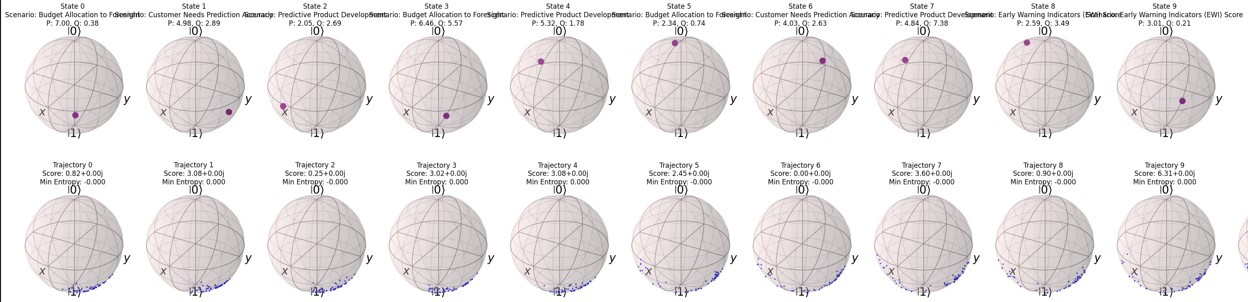
\includegraphics[width=0.8\linewidth]{images/CCQM.jpg}
    \caption{Simulation of a customer centricity analysis with $\phi$QINN}
\end{figure}

The top row of the image shows the evolution of a project's state, represented by a single purple dot on a Bloch sphere, across different milestones (State 0 to State 9). Each state represents the project's status on a given day. The sphere's surface represents a state of perfect certainty, while the interior represents indeterminacy. The purple dot's location within the sphere visually quantifies the project's certainty at that point in time.

\begin{itemize}

    \item \textbf{States of Uncertainty}: In States 1, 3, and 5, the dot moves significantly toward the center of the sphere, indicating a high level of uncertainty in the project's direction. This aligns with RQM's view of projects as non-deterministic systems.

    \item \textbf{Customer-Centricity as a Decision Point}: The labels above the spheres ("Budget Allocation to Needs," "Predictive Product Development") suggest that key business decisions are the events that push the project state. The dot's position reflects the inherent uncertainty of these decisions. For example, in State 2, the "Predictive Product Development" decision has a low P value (0.29), indicating high uncertainty, which is visually confirmed by the dot's position far from the sphere's surface.
\end{itemize}
The bottom row of the image shows multiple possible project trajectories. This is a direct visualization of quantum superposition applied to project management. The blue dots represent the simultaneous existence of all possible outcomes for the project's state.
\begin{itemize}
    \item \textbf{The "Wave Function" of the Project}: Each trajectory shows how the project "wave function" (the collection of blue dots) evolves over time. A scattered group of dots represents high entropy and a broad range of possibilities. A tight cluster of dots, like in Trajectory 1, indicates a more predictable path with less uncertainty.

    \item \textbf{The Role of Entropy}: The Min Entropy value for each trajectory quantifies this spread. Trajectory 0 has a low entropy of 0.00, meaning it is a very stable, predictable path. Trajectory 3, with a higher entropy of 0.05, suggests a more volatile and less certain path.

    \item \textbf{Discriminating Trajectories}: The Score for each trajectory, based on factors like entropy and other metrics, allows managers to discriminate between them. In this RQM framework, the goal is to select the trajectory with the highest probability of success and a manageable level of risk, even if it's not the path with the lowest entropy. The output provides the manager with the information needed to make this decision.
\end{itemize}

A single purple dot on the sphere represents the project's state, with its position indicating the level of certainty: a dot on the surface signifies high certainty, while a dot closer to the center indicates high uncertainty. In this model, both \textbf{bias} and \textbf{noise} can significantly impact our perception of a project's actual state.

Biases are systematic distortions that can skew the assessment of a project's state, often making it appear more certain or stable than it truly is.

\begin{itemize}
    \item \textbf{Cognitive Bias}: The labels above the spheres, such as "Budget Allocation to Needs" or "Predictive Product Development," represent key decisions and assessments. These are susceptible to cognitive biases. For example, \textit{optimistic bias} might lead a project team to overestimate the probability of success ($P$), which would artificially pull the purple dot closer to the sphere's surface (as seen in State 0 where $P=1.00$).
    \item \textbf{Confirmation Bias}: If a team is overly committed to a particular idea, they may interpret data in a way that confirms their pre-existing beliefs. This \textit{confirmation bias} can lead to a "Customer Needs Prediction" that appears more stable than it actually is, even if the underlying data is weak.
    \item \textbf{Anchoring Bias}: The initial budget allocation or other early decisions can act as an anchor, influencing subsequent assessments. This \textit{anchoring bias} can lead to a skewed evaluation of project viability in later stages, even when initial assumptions were flawed.
\end{itemize}

Noise refers to random errors or irrelevant information that introduces variability and distorts the true certainty of a project's state.

\begin{itemize}
    \item \textbf{Data Noise}: The values for $P$ (probability of success) and $Q$ (uncertainty or risk) are derived from data. This data can contain random errors, or "noise." For example, noisy customer feedback can lead to an inaccurate "Customer Needs Prediction" (e.g., $P=0.89$ in State 1) that does not reflect the market's true needs.
    \item \textbf{Measurement Error}: The processes used to assess project parameters, such as the effectiveness of budget allocation, can have inherent measurement errors. This noise distorts the true certainty of the state, making it difficult to pinpoint the project's actual position on the Bloch sphere.
    \item \textbf{Environmental Noise}: Unforeseen external events, such as a sudden market shift, a competitor's actions, or a new regulatory change, can act as environmental noise. These events can increase the indeterminacy of a state, pushing the purple dot toward the center of the sphere even if internal processes are sound.
\end{itemize}

In essence, while the Bloch sphere provides a powerful visualization of project states, understanding the pervasive influence of both bias and noise is critical for accurate interpretation and effective decision-making.


In the context of this decision-making simulation and the score calculation, bias and noise represent sources of uncertainty or error that can affect the quality of a judgment or trajectory.

\begin{itemize} \item \textbf{Bias ($\sigma_{bias}$):} Bias represents a systematic error or a consistent deviation of judgments (points along a trajectory) from an established standard (the final state of the trajectory in this implementation). A high bias indicates that, on average, the trajectory is "off the mark" and not consistently moving towards the intended final state. It is calculated as the square root of the average squared difference between each point in the trajectory and the standard.

\item \textbf{Noise ($\sigma_{noise}$):} Noise, often measured as Mean Squared Difference (MSD) or variance, represents random error or inconsistency in the judgments (points along a trajectory). High noise signifies that the trajectory is erratic and unpredictable, even if the average path might be close to the standard. It is calculated as the square root of the average squared difference from the mean judgment of the trajectory:
$$ \sigma_{noise} = \sqrt{\frac{1}{N} \sum_{i=1}^{N} (\text{Judgment}_i - \overline{\text{Judgment}})^2} $$
where $\text{Judgment}_i$ is the $i$-th point in the trajectory and $\overline{\text{Judgment}}$ is the mean of the points in the trajectory.

\item \textbf{Total Uncertainty ($\sigma_{total}$):} The total effective uncertainty associated with a trajectory is a combination of both bias and noise. It is calculated using a weighted sum:
$$ \sigma_{total} = \sigma_{bias} \cdot w + \sigma_{noise} \cdot (1 - w) $$
where $w$ is a weighting factor ($0 \le w \le 1$) that reflects the prioritization of reducing bias versus reducing noise in the decision process. This total uncertainty is implicitly factored into the original score calculation $S$ that the neural network is trained to predict.

\end{itemize}

The neural network aims to learn the complex relationship between the initial state's characteristics, the trajectory's path (which is influenced by underlying dynamics and potentially noise), and the resulting score S, which itself is a function of factors including the minimum entropy (related to purity) and the time to reach it. By learning to predict S, the network can indirectly account for the impact of bias and noise on the trajectory's quality as measured by the score.
\newpage
\section{Simulation of the Relativistic Quantum Management of a New Insurance Product with $\phi QINN$}
\label{sec9}
As the last application in this thesis, I here describe the simulation of the launch of a new insurance product thus embracing all the previous sections into this.\\
Managing the launch of a new insurance product is a complex process with many moving parts. To handle this, I can use a system that applies Relativistic Quantum Management (RQM) principles to model the entire process. This is not just about using quantum computers for calculations, but about adopting a quantum-inspired mindset to deal with the project's inherent uncertainty.


Imagine the entire product launch journey -from the initial idea to its final market performance- as a global pilot wave. This wave does not follow a single, straight line; instead, it exists in a state of superposition, containing all possible future scenarios at once.
\begin{itemize}
\item \textbf{The Pilot Wave's Journey}: The wave starts at the beginning of the project and moves toward the final goal of a successful product. Along the way, it encounters numerous intermediate states. These are all potential events or outcomes that can happen.
\item \textbf{Bloch Vectors}: The project's intermediate states are represented as Bloch vectors, a mathematical tool from quantum mechanics used to visualize the state of a qubit. Here, they capture the many unexpected events that can occur, such as a regulatory delay or a competitor's surprise launch. Each vector represents a different potential path the project could take.
\item \textbf{Entropy}: The model weighs each of these potential paths based on its entropy. In this context, entropy isn't about disorder; it is a measure of the complexity and accumulated "energy cost" of a particular path. A straightforward path (e.g., no delays, everything goes as planned) has low entropy, while a path with multiple problems (e.g., legal issues, bad market feedback) has high entropy. The model's job is to analyze these entropic costs to find the most probable and efficient routes to success.
\end{itemize}


My quantum-inspired model, called $\phi QINN$, simulates this entire process by mapping the most likely trajectories of the pilot wave from start to finish.
\begin{center}
\begin{tabular}{|p{4cm}|p{6cm}|p{6cm}|}
\hline
\textbf{Step} & \textbf{Description} & \textbf{Key Activities} \\
\hline
\textbf{1. Market Research and Idea Generation} & Identify a market need or gap for a new insurance product. & Analyze market trends, consumer behavior, and competitor products. Brainstorm innovative solutions. \\
\hline
\textbf{2. Product Design and Development} & Define the product's features, target market, and pricing structure. & Determine coverage, benefits, and underwriting guidelines. Conduct actuarial analysis to set premiums. \\
\hline
\textbf{3. Regulatory Approval} & Obtain approval from state or federal insurance regulators. & File policy forms, rates, and marketing materials with regulatory bodies. Ensure legal compliance. \\
\hline
\textbf{4. Product Rollout and Launch} & Introduce the new product to the market. & Conduct a pilot program. Develop and execute marketing and sales strategies. \\
\hline
\textbf{5. Monitoring and Maintenance} & Continuously track and manage the product's performance. & Monitor sales, profitability, and claims data. Adjust pricing or features as needed. \\
\hline
\end{tabular}
\end{center}
\begin{itemize}
\item \textbf{Market Research and Idea Generation}: This is the starting point of the pilot wave. The goal is to identify a market need by analyzing trends and consumer behavior.
\item \textbf{Product Design and Development}: The wave moves into the design phase. This is where potential \textbf{intermediate states} with high entropy can arise. For example, actuarial analysis might reveal that the proposed premiums are not profitable, forcing the team to find a new path.
\item \textbf{Regulatory Approval}: This phase introduces significant uncertainty and potential for high entropy. A regulatory body might ask for changes to the policy forms, adding unexpected time and cost to the project's trajectory.
\item \textbf{Product Rollout and Launch}: The product enters the market, and the pilot wave's trajectory is now influenced by real-world consumer feedback. A poor reception could add more entropy to the path, requiring a quick response.
\item \textbf{Monitoring and Maintenance}: The wave reaches its final destination. The company monitors sales and profitability to ensure the product remains successful. This phase also contains potential high-entropy events, such as a sudden rise in claims that requires a pricing adjustment.
\end{itemize}
By using this approach, a manager can move beyond a simple checklist and proactively guide the product's pilot wave toward a low-entropy, successful outcome.
\newpage
\begin{centering}
\begin{figure}[!h]
    \centering
    \begin{subfigure}[b]{0.45\linewidth}
        \centering
        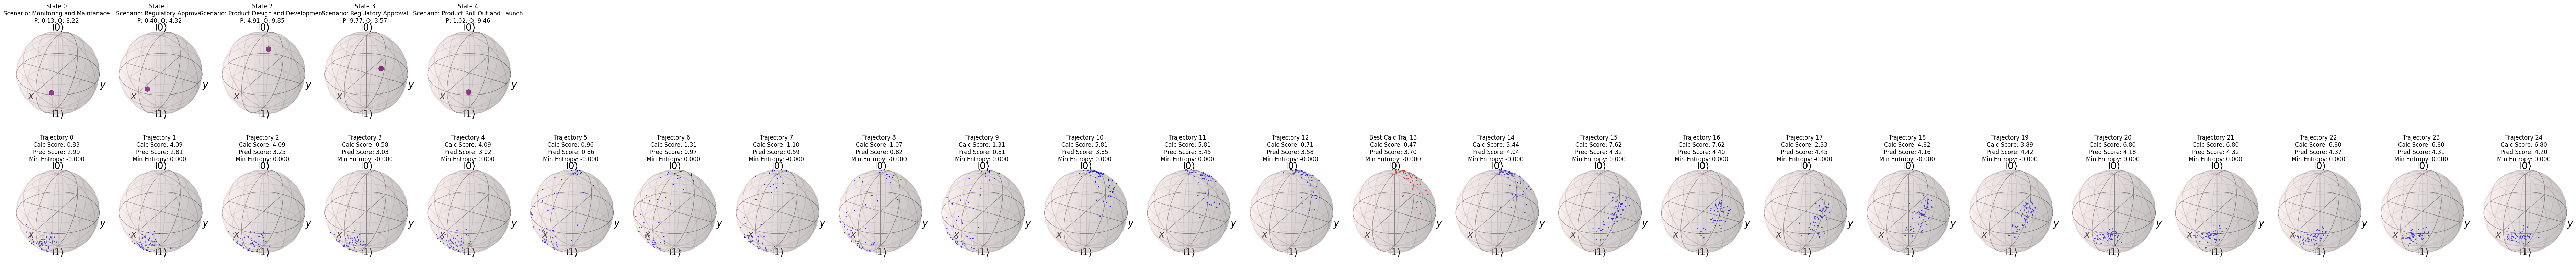
\includegraphics[width=\linewidth]{images/fquinnNewInsProduct(2).png}
        \caption{Relativistic Quantum Management of a New Insurance Product}
        \label{fig:fquinn}
    \end{subfigure}
    \hfill
    \begin{subfigure}[b]{0.45\linewidth}
        \centering
        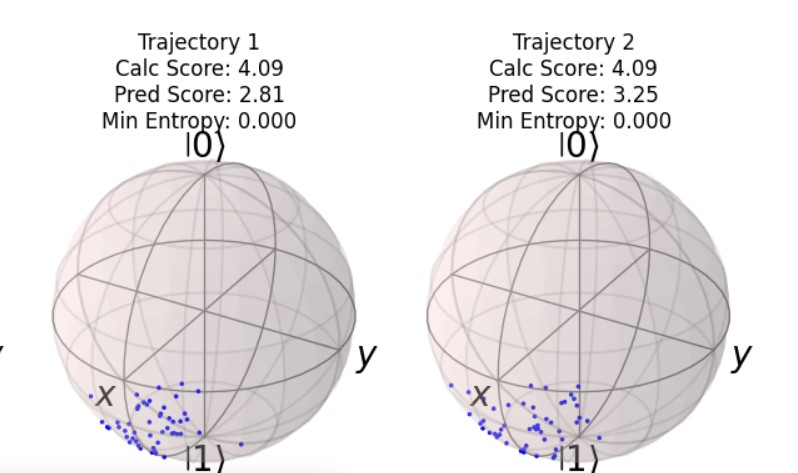
\includegraphics[width=\linewidth]{images/blocks(1).jpg}
        \caption{Relativistic Quantum Management of a New Insurance Product}
        \label{fig:blocks}
    \end{subfigure}
    \par\bigskip % Adds vertical space between rows of subfigures
    \begin{subfigure}[b]{0.45\linewidth}
        \centering
        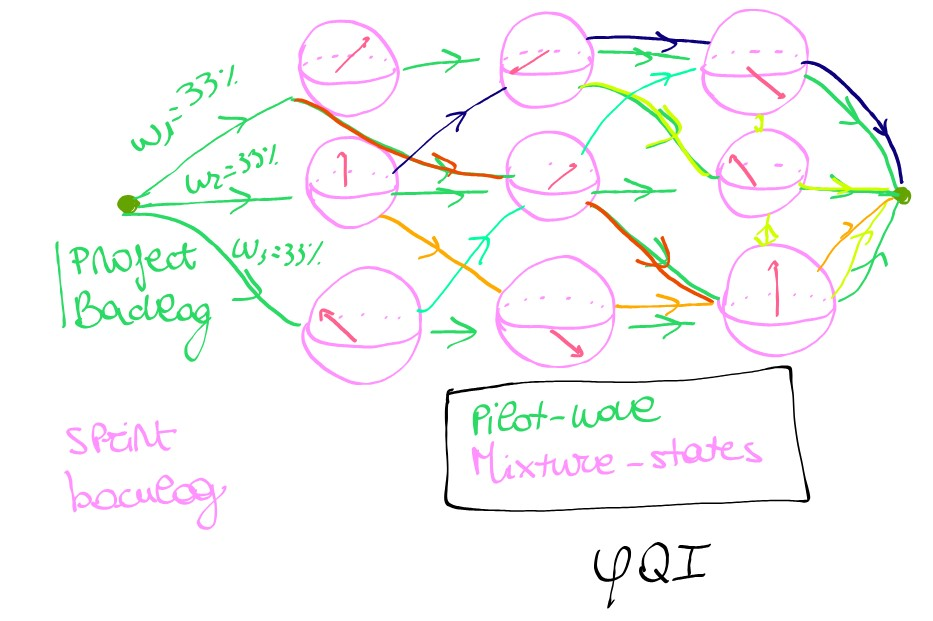
\includegraphics[width=\linewidth]{images/rphqi(1).jpg}
        \caption{Pictorial Representation of Relativistic Quantum Management of a New Insurance Product}
        \label{fig:rphqi}
    \end{subfigure}
    \hfill
    \begin{subfigure}[b]{0.45\linewidth}
        \centering
        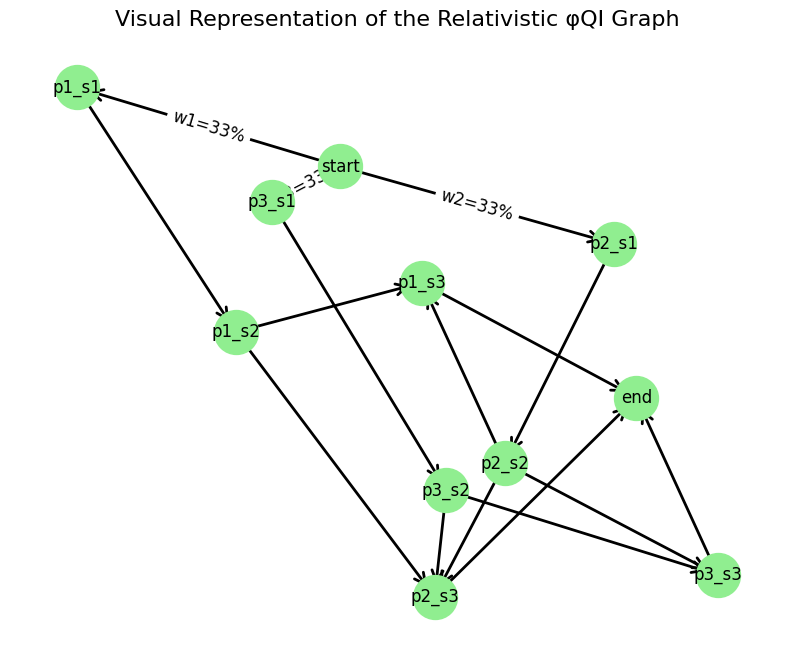
\includegraphics[width=\linewidth]{images/rfqm(1).png}
        \caption{Pictorial Representation of Relativistic Quantum Management of a New Insurance Product}
        \label{fig:rfqm}
    \end{subfigure}
    \caption{A collection of figures illustrating Relativistic Quantum Management concepts.}
    \label{fig:all_figures}
\end{figure}
\end{centering}
The output shows that the model generated many scenarios and simulated 45 possible trajectories or paths through them. Each scenario, like "Workplace Well-being" or "Community Impact," represents a potential state or challenge that a business project might encounter in the development of a New Insurance Product.

\begin{itemize}
\item \textbf{Bloch Spheres as "States"}: The top row of the graph visually represents the all scenarios. Each sphere, known as a Bloch sphere, holds a point (or multiple points) that signifies a project's state of the process.
\item \textbf{Trajectories}: The trajectories represent all the possible sequences of events a project could follow. These are visualized as a scatter of blue dots on the Bloch spheres, each one representing a point along a trajectory.
\item \textbf{Finding the "Best" Path}: The model’s objective is to identify the most favorable path. This is done by calculating a Score S, which is a metric that is meant to be minimized. This score is directly related to entropy, a concept that measures a project's complexity and disorder.
\end{itemize}
The model successfully identifies the best trajectory, which has a minimal Score S.\\\\ This shows the potentiality of the RQM approach: it can navigate a huge number of potential outcomes to pinpoint the single most efficient and stable path, reducing complexity and risk while considering uncertainty, indeterminism and relativity.\\Because of its flexibility with initial conditions, this model could be potentially applied to any process, in any field.
\newpage
\section{Conclusions}
In summary, the field of Relativistic Quantum Management, derived from Quantum Management by Danah Zohar, investigates a fundamental question:
\begin{center}
\begin{equation}
    \text{How is information processed by all parts of an organization in case of uncertainty and indeterminism?}
\end{equation}
\end{center}
To explore this, a compelling analogy has been drawn from the world of physics.\\
Physics indeed covers a key role in the analogy because of its classical and quantum areas. In particular, the first one can be used to describe the Newtonian Management, while the second one to describe a more uncertain and nondeterministic framework, such as Quantum Management.
In physics, we also have the honor to deal with a wonderful theory "Special Relativity" by Einstein that has been here considered for an analogy with what I called "Relativistic Quantum Management".  In the recent physics, a higher precision is required to discover new physics: it can happen, for example, that new physics is hidden behind signals due to bad measured or treated uncertainties. The dealing with these uncertainties a critical endeavor \cite{NNPDF:2021njg}. 

Management, by its way, saw a development through the history that can be analog to the development of physics through the history. Management and physics can therefore be dealt on the same plane as they both abstract a problem and/or a process. A good manager can be compared to a good (theoretical and experimental) physicist:
if, from the theoretical point of view, the manager should be able to formalize what is happening, see a potential problem and/or deal directly with it, understand and read people and their talents, other than their needs, or to draw a line to follow. 

A good theoretical physicist should be able to write a Lagrangian and all the necessary ingredients to write a complex theory that requires the acknowledgment of conditions, of equations and the formalism to use to find the answer that is looked for; From an experimental point of view, a good manager, as an experimental physicist, should be able to properly deal with uncertainties and with errors, with measurements and the proper experimental apparatus that is able to measure what is looked for.

In the end, a good manager as a good physicist is able to see what others do not see in order to recognize the problem, the question to make and the answer to find. This is a job that requires critical thinking, problem solving, imagination and abstraction that go in a horizontal and a vertical directions.
\begin{comment}
\begin{tabularx}{\textwidth}{l|X|X}
    \toprule
    & \textbf{The Theoretical Manager} & \textbf{The Theoretical Physicist} \\
    \midrule
    \textbf{Problem Formulation} & Formalizes business problems, identifies root causes, and anticipates challenges. & Writes a Lagrangian, defining the system's energy and potential interactions. \\
    \midrule
    \textbf{System Understanding} & Understands people's talents, motivations, and needs. & Acknowledges initial conditions, equations of motion, and physical laws. \\
    \midrule
    \textbf{Strategic Planning} & Draws a clear line to follow, a strategic roadmap for the team. & Uses the formalism and theory to derive the equations and solutions needed to find the answer. \\
    \midrule
    \textbf{Shared Skill} & \multicolumn{2}{c}{\textbf{Critical thinking} and \textbf{abstraction} to see what others miss.} \\
    \hline
    \textbf{Measurement \& Data} & Properly deals with performance metrics, feedback, and market data. & Uses a proper experimental apparatus to measure what is being studied. \\
    \midrule
    \textbf{Uncertainty \& Error} & Manages a project's inherent uncertainties, risks, and potential errors. & Deals with measurement uncertainties and systematic errors, which can obscure results. \\
    \midrule
    \textbf{Implementation} & Executes strategies and adjusts based on real-world feedback. & Runs experiments and analyzes data to either validate or refute a theory. \\
    \midrule
    \textbf{Shared Skill} & \multicolumn{2}{c}{\textbf{Problem-solving} and \textbf{imagination} to devise a plan and execute it.} \\
    \bottomrule
\end{tabularx}
\end{comment}
A great manager uses a kind of "applied mathematics" to formalize and solve business challenges. This isn't about running complex equations, but about using logic, data analysis, and abstract reasoning to model a system's reality. By doing so, they can identify hidden patterns, anticipate future problems, and devise strategies that seem counterintuitive but ultimately prove successful. 


My investigation of the analogy between quantum management and quantum mechanics and quantum field theory has been inspired by the need to combine the indeterminism and the uncertainty of quantum mechanics with the special relativity theoretical framework, in terms of existing mathematical and theoretical tools. These ones are Feynman Path Integral, the De Broglie Pilot Wave and the Von Neumann Density Matrix.

By using Feynman Path Integrals, I can account for the multitude of events that could occur from the beginning of the process to the end of sprint backlogs. This approach sums all possible trajectories between intermediate states of uncertainty, effectively exploring every potential outcome. Each of these intermediate states can be represented by density mixture states, which correspond to the various phases of a process and sprint backlogs.

While the pilot wave guides the overall direction, that corresponds to the project backlog, the path integral explores all possible deviations and detours. What I try to look for is the best trajectory, given some initial conditions.

From Statistical Mechanics, I thought that the most effective path is the one that minimizes entropy, as entropy serves as a measure of disorder within a system. 

By seeking the trajectory that leads to the lowest entropy, I am identifying the most ordered and efficient route from the initial state to the final outcome. This allows to navigate the complexities of uncertainty, indeterminism and relativity while still striving for a clear, predictable, and successful result.

The fundamental equation of this formalization is the following:
\begin{equation}
    \phi \epsilon \rho \omega = \int \mathcal{D}scenario \exp\left( \frac{i}{\text{Quantum Term}} Action[scenario] \right)
\end{equation}

This is in particular inspired by the Feynman Path Integral and it can be applied to every context of a certain process. In this case, I considered the insurance sector, but it could be extendable to every field.

In this thesis, in the context of leadership, asset management, esg principles and customer centricity, I drew some quantum terms that replace the quantum term ($\hbar$) which are:
\textbf{adaptiveness, realism, balance and proactivity}.

If each one goes to zero, it brings back to a Newtonian management of the process, similarly to a classical limit in physics.

The best trajectory, the one that minimizes the entropy, is thought to travel among many scenarios of intermediate states, with start and end points well posed ab initio, as a travel from Turin to Madrid. If the cities are apprixomately always in the same position, the way to reach them can be different. It is possible that the trajectory by plane is the one that reduces entropy as it is the fastest and the most linear one.

To effectively apply the Relativistic Quantum Management, it is also essential to categorize and recognize the sources of uncertainty within an organization. While it is imperative to deal with uncertainty, it is equally important to manage indeterminism, as noted by Danah Zohar in her work \cite{zohar2021zerodistance}. Indeterminism, unlike uncertainty, refers to a state where an outcome is not predetermined, necessitating a different approach to strategic planning and decision-making.\\\\
Relativistic Quantum Management, while embracing indeterminism, uncertainty and relativity, looks for the harmony of the process that corresponds to the best trajectory.\\\\Similarly to ”Gli Effetti del Buon Governo” by Lorenzetti, is inspired by The Governo dei Nove (Government of the Nine)
that was one of the main magistracies of the Republic of Siena, in power from 1287 to 1355. The fresco is structured in three
registers: the upper one with divine components (Divine Wisdom and the Theological Virtues); the middle one with the
city’s institutions (Justice, the Commune, and the Cardinal Virtues); and the lowest one with the builders and beneficiaries
of these institutions (the army and the citizens). The rope symbolizes the union between Justice and the Commune, which
are inseparable and useless without each other. The citizens, in a state of harmony, hold them together.
Harmony is what Relativistic Quantum Management aims for by adopting a dynamical and skeptical aptitude. From
this point view, the fresco shows the ”what” (a virtuous government and its effects), while the quantum model explains the
”how” (how to manage interconnectedness and uncertainty to maintain the fluidity and adaptability needed to prosper).
Essentially, Lorenzetti’s Good Government is the perfect metaphor for the stability a company seeks, but Quantum
Management could be interpreted as the operational philosophy that recognizes this stability is not static; rather, it’s a
dynamic equilibrium that must be continuously renewed.

In the Insurance sector, in this era, there are Nine challenges to deal with Data Quality: Ensuring the quality of data
that describes the company’s (and group’s) situation and its target markets is crucial. This involves formalized data quality
processes that are subject to auditing. Characteristic Metrics: Producing values for key metrics like ”best estimate liability,”
”Solvency Capital Requirement” (using the standard formula and/or internal model), and ”Technical Provisions.” Validation
and Accuracy: Performing accuracy, robustness, and market consistency tests as defined and required by regulations (e.g.,
IVASS Regulation no. 18 of March 15, 2016, articles 57 and 58). Regulatory Reporting: Producing metric values for the
Quantitative Report Templates (QRTs). Risk and Solvency Assessment (ORSA): Supporting the Own Risk and Solvency
Assessment (ORSA) process with functionalities that allow for the ”experimentation” of business strategies and capital
allocation. PRIIPs: Producing metric values and technical ratios for the Key Information Document (KID) for Packaged
Retail and Insurance-based Investment Products (PRIIPs), IFRS17 Compliance: Producing sets of metrics that conform
to IFRS17 conventions to be transferred to the company’s ”accounting system” and Informational Reports: Generating
informational reports at different levels of detail for various organizational units, technical committees, senior management,
and the board of directors. Ways to face for a ”new way of doing insurance” are: Market consistency, Risk Management,
New Model, Data Quality, High Technology, Training and Governance \cite{sfide9}.

Relativistic Quantum Management could be used by addressing these challenges through a framework that accounts for the dynamic, interconnected nature of data and risk, the insurance sector can achieve a state of dynamic equilibrium, moving beyond static, linear processes toward a more fluid and responsive operational model.

The transition to a new management paradigm is not merely about changing processes, but fundamentally about shifting the mindset that guides decision-making. Humans need support in making decisions and must be aware of the underlying mental models they are applying.

The new mindset for management should evolve in a manner analogous to the historical development of management theories. This journey begins with a rigid, linear approach, then curves to encompass complexity, expands into a new dimension of multi-faceted interaction, and ultimately operates interactively in space-time. This conceptual evolution can be understood through the ancient and powerful symbol of the circle. The circle indeed is a potent and ancient symbol in philosophy, representing unity, eternity, perfection, and cyclicality. Its properties—lacking a beginning or end and having all points equidistant from a center—have made it a universal metaphor.

    Vicious and Virtuous Circles: In a practical sense, the circle illustrates feedback loops. A vicious circle describes a negative, self-reinforcing chain of events where solutions worsen the problem. Conversely, a virtuous circle represents a positive feedback loop where each improvement builds upon the last, leading to continuous progress.

    Existential and Epistemological Circles: Philosophers have also used the circle to explore deeper concepts. Friedrich Nietzsche's idea of Eternal Recurrence frames life as a cycle of repetition, while the hermeneutic circle describes the iterative process of understanding a text or concept by moving between its parts and the whole.

    The Circle of Completion: In psychology, Carl Jung viewed the circle as a symbol of psychological completion or Individuation. This process represents the journey toward a fully integrated, whole self.

Essentially, this new management mindset must move beyond linear thinking to embrace a circular, dynamic, and interconnected worldview. Just as the circle symbolizes unity and continuous motion, the ideal mindset for a relativistic quantum approach must be one of constant adaptation and integration, recognizing that every action has feedback that influences the entire system.

Zohar's "quantum paradigm" offers a solution to undeterminism by shifting our perspective from a rigid, mechanical worldview to one that sees individuals, organizations, and societies as complex, self-organizing, and interconnected systems. This change is crucial for preventing hysteresis \cite{elster_review_georgescu-roegen_1977}, \cite{author_name_2024_conservative}, a phenomenon that describes a system's dependence not only on its current state but also on its past history. In physics, a ferromagnetic material retains a residual magnetic state even after the external magnetic field is removed.\\
In a similar vein, social systems—be they individuals, organizations, or entire societies—can continue to operate based on "past answers" and outdated paradigms long after the original conditions have vanished. This raises a critical question: 
\begin{center}
\begin{equation}
    \text{How long can a system continue to respond to new events with solutions from the past?}
\end{equation}
\end{center}
This persistent reliance on historical methods creates a significant lag in our collective response, leaving us "out of sync" with present realities. This intellectual and behavioral inertia could be a major obstacle to progress and innovation. A fluid \cite{bauman2000liquid}, quantum-inspired approach aims to overcome this inertia by promoting a mindset of continuous adaptation and renewal, rather than clinging to outdated, linear solutions.
\newpage
\bibliographystyle{unsrt}
\bibliography{ref}
\newpage
\begin{figure}
    \centering
    
\includegraphics[width=0.5\linewidth]{images/960px-Piero_della_Francesca_046.jpg}
    \caption{Sacra Conversazione, Piero della Francesca}
    \label{fig:placeholder}
\end{figure}
\end{document}
